\documentclass[12pt,twoside]{article}

% Indicaciones para el idioma:
\usepackage[T1]{fontenc}
\usepackage[utf8]{inputenc}
\usepackage[spanish]{babel}

% Adaptación de itemize y enumerate a los usos tipograficos españoles:
\let\layoutspanish\relax
\addto\captionsspanish{\def\tablename{Tabla}} % para que escriba "Tabla" en lugar de "Cuadro"
\unaccentedoperators  % para que no acentúe los operadores

% Área de impresión de una página:
\usepackage[a4paper]{geometry}
  \geometry{hmargin={2.5cm,2.5cm},height=22cm}

% Formato de algunas distancias:
\renewcommand{\baselinestretch}{1.2}    % separación entre líneas de un mismo párrafo
\setlength{\partopsep}{0pt}
\setlength{\itemsep}{0pt}
\setlength{\topsep}{0pt}
\setlength{\parsep}{0pt}
\setlength{\parskip}{0.25\baselineskip}   % separación entre párrafos

\renewcommand{\textfraction}{0.1}   % mínima fracción de la página para el texto
\renewcommand{\topfraction}{1}      % máxima fracción de la página para objetos flotantes en la parte superior
\renewcommand{\bottomfraction}{1}
\renewcommand{\floatpagefraction}{1}

\setcounter{totalnumber}{5}
\setcounter{topnumber}{3}
\setcounter{bottomnumber}{2}

% Adaptación de las "caption" de los entorns "figure" y "table":
\usepackage{caption}
\captionsetup{
  labelfont={up,bf},%
  font={small,sl},%
}

% Indentación del primer párrafo de una sección:
\usepackage{indentfirst}

\usepackage{makecell}

% Definición del color grisclaro en la salida PDF:
\usepackage[pdftex]{color}

% Gráficos:
\usepackage[pdftex]{graphicx}

% Paquetes recomendados para la inclusión de fórmulas matemáticas:
\usepackage{amsmath}
\allowdisplaybreaks  % para que pueda partir fórmulas que ocupan más de una línea, necesita el paquete anterior
\usepackage{amssymb} % para cargar algunos símbolos como \blacksquare y \square
\usepackage{amsfonts} % para cargar algunas fuentes en estilo matemático
\usepackage{enumerate}

% Teoremas (se pueden definir todos los que se necesiten):
\newtheorem{theorem}{Teorema}[section]
\newtheorem{proposition}[theorem]{Proposición}
\newtheorem{definition}[theorem]{Definición}
\newtheorem{lemma}[theorem]{Lema}
\newtheorem{corollary}[theorem]{Corolario}
\newtheorem{example}[theorem]{Ejemplo}
\newtheorem{app}[theorem]{Aplicación}
\newtheorem{remark}[theorem]{Observación}
\newtheorem{agrad}[theorem]{Agradecimiento}
\newtheorem{algo}[theorem]{Algoritmo}
\newtheorem{axiom}[theorem]{Axioma}
\newtheorem{case}[theorem]{Caso}
\newtheorem{conclu}[theorem]{Conclusión}
\newtheorem{conjectura}[theorem]{Conjetura}
\newtheorem{notac}[theorem]{Notación}
\newtheorem{soluc}[theorem]{Solución}
\newtheorem{summary}[theorem]{Sumario}


\newtheorem{proof}[theorem]{Demostración.}
\renewenvironment{proof}{\emph{Demostración.}} {\quad \hfill $\blacksquare$ \newline} % para que aparezca un cuadrado negro al acabar la demostración


% Definición de cabeceras y pies de página:

\usepackage{fancyhdr}      % para definir distintos tipos de cabeceras y pies de página

\usepackage{amssymb} % para cargar algunos símbolos como \blacksquare y \square
\usepackage{pifont} % para \xmark
\newcommand{\xmark}{\ding{55}}

\newcommand{\RunningAuthor}{Juan Francisco Correas Díaz}
\newcommand{\Author}[1]{\renewcommand{\RunningAuthor}{#1}}
\renewcommand{\leftmark}{\RunningAuthor}

\newcommand{\RunningTitle}{Trabajo de fin de grado}
\newcommand{\Title}[1]{\renewcommand{\RunningTitle}{#1}}
\renewcommand{\rightmark}{\RunningTitle}

\pagestyle{fancy}
\fancyhf{}
\fancyhead[LO]{\small \slshape \leftmark}    % lo que aparece en la parte izquierda de la páginas impares
\fancyhead[RE]{\small \slshape \rightmark}   % lo que aparece en la parte derecha de las páginas pares
\fancyhead[RO,LE]{\small \slshape \thepage}  % el número de página aparece en la parte exterior de la cabecera

\renewcommand{\headrulewidth}{0.6pt}         % grueso de la línea horizontal por debajo de la cabecera de la página
\renewcommand{\footrulewidth}{0pt}           % grueso de la línea horizontal por encima del pie de página
                                             % en este caso está vacío
\setlength{\headheight}{1.5\headheight}      % aumenta la altura de la cabecera en una parte y media

\fancypagestyle{plain}{%                     % redefinición del estilo de página 'plain'
  \fancyhf{}                                 % limpia todas las cabeceras y pies de página
  \setlength{\headwidth}{\textwidth}
  \fancyfoot[C]{\small \slshape \thepage}    % excepto el centro del pie de página
  \renewcommand{\headrulewidth}{0pt}
  \renewcommand{\footrulewidth}{0pt}
  }

% Instrucciones que se usan frecuentemente
\newcommand{\abs}[1]{\ensuremath{|#1|}}

% Datos del trabajo y autor:
\title{Trabajo de fin de grado}
\author{Juan Francisco Correas Díaz \\*[1em]
\begin{minipage}{0.75\textwidth}
\footnotesize \itshape
\begin{center}
Universidad de Alicante \\
4º de Grado en Matemáticas
\end{center}
\end{minipage}
}
\date{Julio 2025}

% Para incluir paginas de otro pdf (por ejemplo, la de la portada):
\usepackage{pdfpages}

% Para poner enlaces
\usepackage{hyperref}

\begin{document}

% Para introducir la portada en castellano, se guardar anexo-1-portada-memoria-tfg-matematicas.pdf en el mismo directorio:

\includepdf[pages=1]{portada_final.pdf}

\newpage

% Después de la portada, se introducirá un resumen del Trabajo Fin de Grado (máximo 500 palabras) en una de las lenguas oficiales y en inglés, junto con las palabras clave (de 3 a 5).


\section*{Resumen}

Las series temporales siempre han sido uno de los principales temas de estudio a la hora de realizar predicciones a futuro. Coloquialmente, se puede definir una serie temporal como una sucesión de datos en orden cronológico. Dada la masiva cantidad de información que se genera en la actualidad, se buscan constantemente nuevas formas de usarla.

En este trabajo, se han estudiado diferentes modelos de series temporales, desde un punto de vista teórico hasta una visión práctica de los mismos.

En primer lugar, se comienza presentando las definiciones introductorias para contextualizar el trabajo y los procesos clásicos de series temporales. En concreto, se han introducido  los modelos ARIMA para poder tratar los modelos SARIMA.

En segundo lugar, el trabajo se centra en un modelo predictivo reciente: el modelo \textit{Prophet}. Se verá su eficiencia para modelar datos con fuertes relaciones estacionales y el porqué, a día de hoy, sigue siendo uno de los primeros modelos a tener en cuenta cuando se pretende predecir una serie temporal.

A continuación, se tratan teóricamente las Redes Neuronales para introducir las Redes Neuronales Recurrentes, que son un tipo de redes neuronales diseñadas para procesar datos que siguen un orden secuencial. Así, se finaliza la sección con la explicación teórica y puesta en práctica del modelo LSTM, que son un tipo de redes neuronales recurrentes específico cuyo objetivo es suplir las limitaciones de las mismas. 

Posteriormente, se aborda \textit{NeuralProphet}, un modelo de reciente creación que combina el modelo \textit{Prophet} y redes neuronales. Principalmente, este modelo se beneficia de la interpretabilidad y capacidad para captar estacionalidades del modelo \textit{Prophet} y de la flexibilidad para modelar relaciones no lineales de las redes neuronales.

Finalmente, se han comparado los distintos modelos con datos con y sin ruido para comprobar su precisión en las predicciones, resumiendo sus principales diferencias. Se ha desarrollado un proyecto en \textit{Python} para comprobar la eficacia de los modelos y estudiar su implementación en \textit{Python} con datos relacionados con el tráfico aéreo en EE.UU., cuyo código puede consutarse en el repositorio público de \textit{GitHub} del autor.

\textbf{Palabras clave:} SARIMA, \textit{Prophet}, Redes Neuronales, LSTM, \textit{NeuralProphet}.

\newpage

\section*{Abstract}

Time series have always been one of the main fields studied when it comes to forecasting the future. Colloquially, time series can be defined as a sequence of data in chronological order. Due to the massive amount of data being generated everyday, there are constant efforts being made to find new ways to use it.

In this project, different models of time series have been studied from both a theoretic and practical point of view. 

Firstly, basic definitions have been given in order to contextualize the project and the most elemental processes regarding time series. Specifically, ARIMA models have been briefly introduced in order to work with SARIMA models. 

Secondly, this project focuses on a recent predictive model known as \textit{Prophet}. The aim is to show its efficiency in modelling data with strong seasonal relationships and illustrate the reason why it continues to be at the forefront when it comes to the prediction of time series. 

Moreover, a theoretic framework about Neural Networks is presented in order to introduce Recurrent Neural Networks, which are types of neural networks designed to process data indexed in chronological order. Finally, this section introduces a theoretic explanation and practical demonstration of the LSTM model, which is a specific type of recurrent neural network whose aim is to make up for the limitations of said recurrent neural networks. 

Subsequently, one last model, which is a combination of the \textit{Prophet} model and neural networks named \textit{NeuralProphet}, is discussed. This model mainly works with the ability to interpret and capture seasonality present in the \textit{Prophet} model and the flexibility to model non-linear relationships present in neural networks. 

Finally, a comparison between the different models including data with and without noise is made in order to check their precision accuracy, summarising their main differences. A \textit{Python} project has been developed to test the effectiveness of the models and study their implementation in \textit{Python} with data related to air traffic in the USA, whose code can be found in the author’s public GitHub repository.

\textbf{Key words:} SARIMA, \textit{Prophet}, Neural Networks, LSTM, \textit{NeuralProphet}.


% A continuación, se incluirá el índice del trabajo y, seguidamente, se desarrollará la memoria.
\newpage

\tableofcontents

\newpage

\section{Introducción}\label{sec:1}

A lo largo de la historia, el ser humano ha buscado transformar la realidad en que ha vivido. Desde el descubrimiento del fuego hasta la Revolución Industrial, siempre ha tratado de mejorar su forma de vida desarrollando los recursos de los que se disponía. Desde el siglo XVIII hasta hace no mucho, se ha experimentado un gran auge en el ámbito económico y tecnológico, caracterizado por el uso de máquinas y la producción en masa. 

A día de hoy, nos encontramos en plena Revolución Tecnológica. La digitalización, la automatización y la inteligencia artificial están sentando las bases de lo que será un futuro cada vez menos lejano. Todo esto tiene como consecuencia la cantidad masiva de información que se genera y almacena cada segundo. La capacidad de capturar, procesar y analizar datos se ha convertido en uno de los desafíos para el avance de la ciencia, la economía y la sociedad en su conjunto.

Así pues, surge la siguiente cuestión: ¿qué se puede hacer con toda esta información? La Ciencia de Datos juega un papel clave para tratar con estas cantidades ingentes de información y dar pie a un uso práctico de las mismas.

A lo largo del siglo XX, se empezaron a  desarrollar tratamientos para el análisis de series temporales. Destacan los modelos tradicionales ARIMA y SARIMA, pues han proporcionando herramientas matemáticas sólidas para gestionar dichos tratamientos. Sin embargo, con el grotesco crecimiento de la información y la complejidad de fenómenos a modelar, estos enfoques resultan superados.

Con el fin de suplir las limitaciones de los modelos más tradicionales, surgen otros nuevos como \textit{Prophet}. Este modelo permite manejar diversas estacionalidades complejas, lo que resulta interesante en contextos donde los datos presentan variaciones significativas a lo largo del tiempo, como en ventas. Además, se caracteriza por su robustez ante datos faltantes y anomalías y por permitir añadir eventos o festivos al modelo, mejorando así la precisión en las predicciones. 

No obstante, con el incipiente auge del \textit{Machine Learning} en el campo de las series temporales y muchos más, las redes neuronales han demostrado ser grandes aliadas en la predicción de series temporales por su capacidad para modelar relaciones no lineales y para adaptarse a secuencias de diferentes longitudes y características. En particular, las redes neuronales recurrentes (RNN) y sus variantes, como LSTM, han sido diseñadas para capturar relaciones en los datos e introducir conexiones de retroalimentación.

Por todo ello, \textit{NeuralProphet} emerge como un modelo híbrido que combina la estructura de \textit{Prophet} con técnicas de \textit{Machine Learning} (redes neuronales) para proporcionar modelos más robustos y complejos, que vayan más allá de lo tradicional. Por consiguiente, en este trabajo se revisarán brevemente los modelos más tradicionales, se estudiará el modelo \textit{Prophet} y se contextualizará el mundo de las Redes Neuronales juntos con las redes LSTM para dar a paso al modelo \textit{NeuralProphet}. Finalmente, se compararán estos métodos en diferentes situaciones, a partir del mismo conjunto de datos, para analizar las oportunidades y limitaciones de cada uno. Se ha desarrollado un proyecto en \textit{Python} para comprobar todo ello y estudiar su implementación en \textit{Python},  cuyo código puede consutarse en el repositorio público con enlace \textit{GitHub} (\url{https://github.com/juanfran12345/TFG}.

\subsection{Tráfico aéreo mensual de EE.UU. desde 2003 hasta 2023} \label{sec:2}

Estamos en un momento de la humanidad en que la masificación de información y sus tratamientos están suponiendo grandes avances a nivel tecnológico. Con la globalización en que nos encontramos, el numéro de vuelos se ha disparado considerablemente, ya sea por ocio, por fines comerciales o de cualquier otra índole. De una forma u otra, cada vez está más al alcance de cualquier persona la posibilidad de tomar un avión en cualquier momento. 

En el contexto de los datos del tráfico aéreo, el análisis de series temporales puede utilizarse para predecir el número futuro de pasajeros aéreos basándose en datos históricos, lo que puede ayudar a la capacidad de planificación, las estrategias de fijación de precios y otras decisiones comerciales. Ahí es donde entra el \textit{Data Science} y donde pueden ser muy útiles los algoritmos mencionados anteriormente, para intentar analizar distintas estrategias. 


Así pues, para poner a prueba estos métodos, se va a utilizar un conjunto de datos denominado \textit{U.S. Airline Traffic Data (2003-2023)}. Se encuentra en \textit{Kaggle} y está a disposición de cualquier usuario (\href{https://www.kaggle.com/datasets/yyxian/u-s-airline-traffic-data}{https://www.kaggle.com/datasets/yyxian/u-s-airline-traffic-data}). Se trata de un conjunto de datos sobre el tráfico aéreo mensual de EE. UU., desde 2003 hasta 2023. Es un conjunto de datos bastante complejo, pero se han escogido principalmente la variables de tiempo y el número de pasajeros totales que voló cada mes en Estados Unidos.

\begin{figure}[h]
    \centering    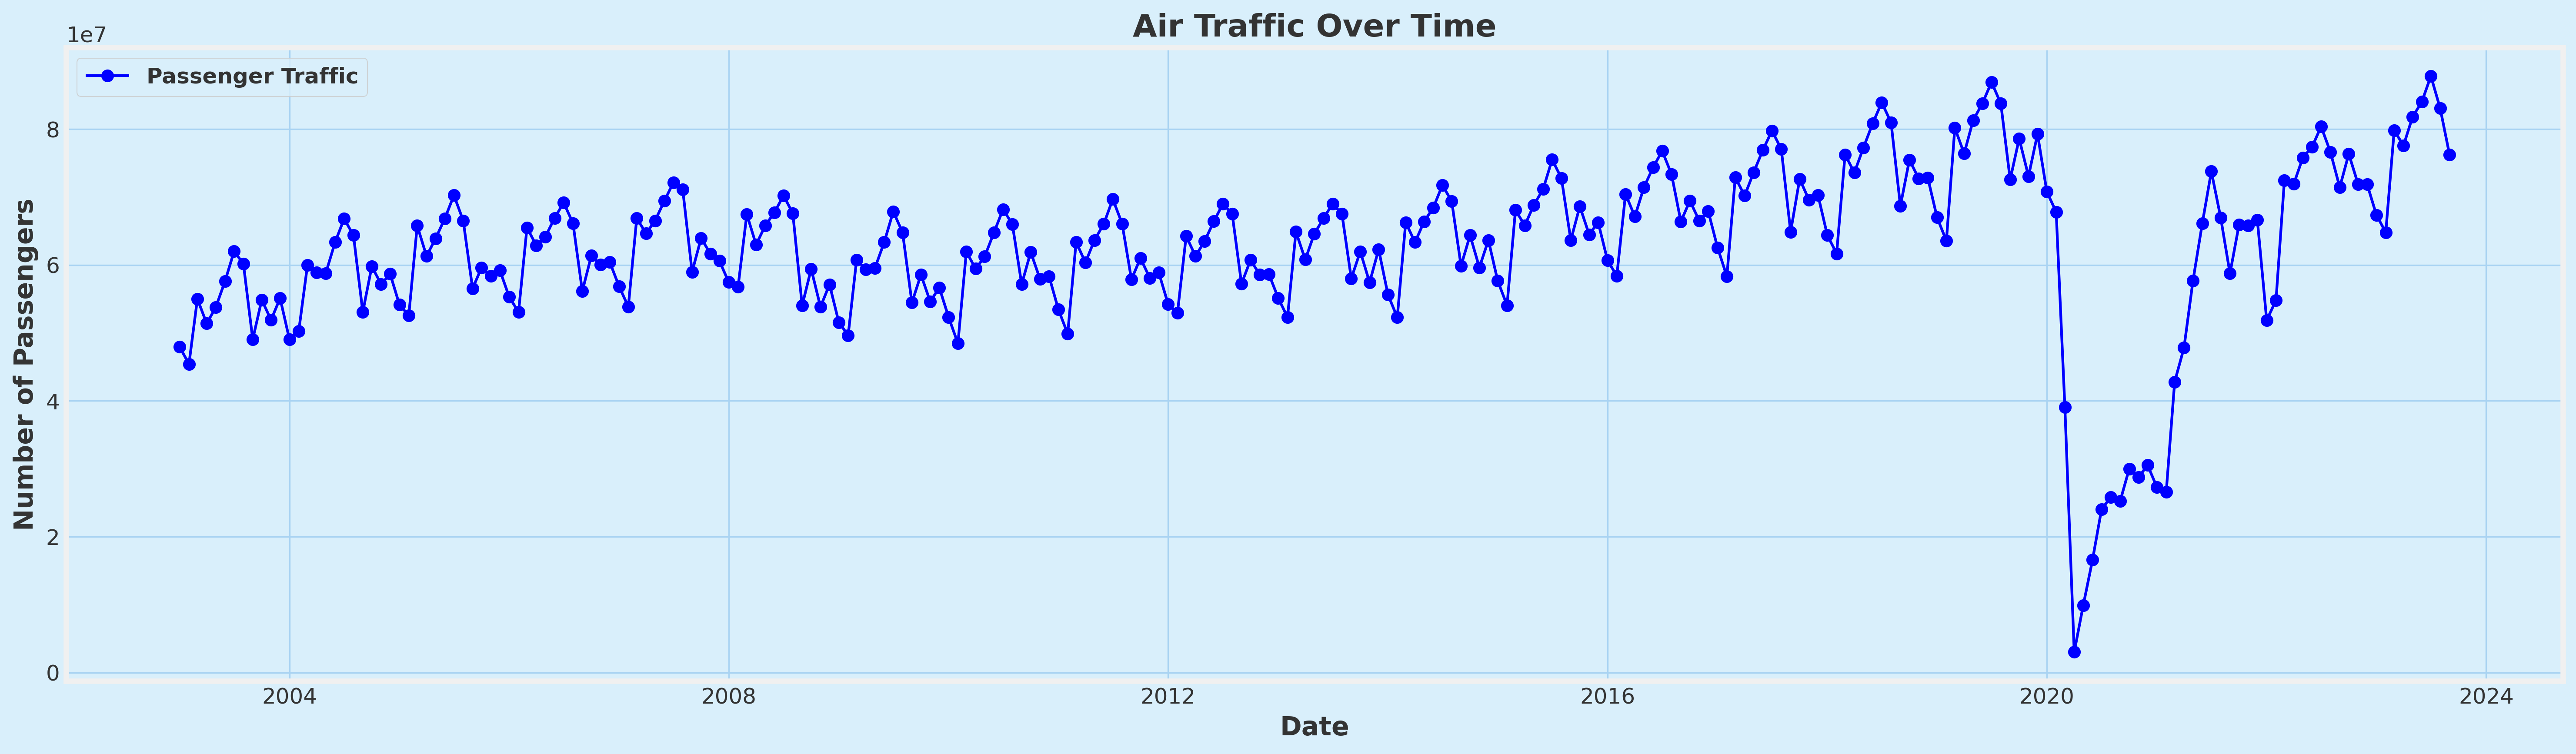
\includegraphics[width=0.8\textwidth,height=0.3\textwidth]{intro.png}
    \caption{Gráfica de la serie temporal}
    \label{fig:fig41}
\end{figure}

En la Figura $~\ref{fig:fig41}$, se puede ver la totalidad de los datos de la serie temporal. Se observa una tendencia creciente en el número de pasajeros a lo largo del tiempo, junto a u patrón estacional que se repite cada año. Se aprecia el impacto que tuvo el COVID en estos datos: la disminución de demanda que conllevó entre los años 2019-2020 y su recuperación en los años siguientes. Por tanto, supone un reto intentar modelar el número de pasajeros para los años siguientes.

La intención de este trabajo es encontrar modelos capaces de adaptarse a los datos y fluctuaciones en ellos. Para retarlos, se va a considerar este conjunto de datos como si fueran dos: se tomará un conjunto de datos que esté comprendido entre 2003 y 2019 (primer conjunto de datos), y otro entre 2003 y 2023 (segundo conjunto de datos), para ver cómo la influencia del COVID-19 afecta a los modelos de series temporales. 

Se dividirán ambos \textit{data sets} en dos: un conjunto de entramiento y un conjunto de testeo o prueba. Para el primer \textit{data set}, se considerará como conjunto de entrenamiento los datos desde 2003 hasta 2017, inclusive, y como conjunto de testeo los restantes. Por su parte, para el segundo \textit{data set}, se considerará como conjunto de entrenamiento los datos desde 2003 hasta 2021, inclusive, y como conjunto de testeo el resto. 

\subsection{Evaluación y comparación de modelos}

Con el fin de testar los modelos, se llevarán a cabo dos métricas que ayudarán a seleccionar los mejores modelos de series temporales con los que se trabajarán. En primer lugar, para hacer las predicciones se supondrá que se observa una serie temporal $\{X_t\}_{t=1}^{T}$, con $T \in \mathbb{N}$, y que se desea predecir $X_{T+h}$, con $h \in \mathbb{N}$. Las métricas de las que se hará uso son el Error Cuadrático Medio (MSE) y el Error Absoluto Medio Porcentual (MAPE), que se expresan de la siguiente forma: 

\begin{equation}
\mathrm{MSE} = \frac{1}{T} \sum_{t=1}^{T} (y_t - \hat{y}_t)^2
\end{equation}

\begin{equation}
\mathrm{MAPE} = \frac{100}{T} \sum_{t=1}^{T} \left| \frac{y_t - \hat{y}_t}{y_t} \right|,
\end{equation}

donde $y_t$ son los valores reales e $\hat{y}_t$ son los valores predichos para el instante de tiempo $t \in \{1,...,T\}$.

Por consiguiente, para evaluar cada modelo se utilizará la métrica MAPE sobre el conjunto de entrenamiento y de testeo. Para seleccionar el mejor modelo en cada sección y para cada \textit{data set}, se compararán los datos del conjunto de testeo con las predicciones resultantes del conjunto de entrenamiento y se elegirá aquel que menor error MAPE tenga para el testeo.

Además, se usará el error MSE para obtener los mejores parámetros en el conjunto de entrenamiento para cada modelo, y se llevarán a cabo las predicciones usando estos mejores parámetros. Como se ha comentado, se elegirán los mejores parámetros sobre el conjunto de entrenamiento, pero también existe la posibilidad de tomar un subconjunto del conjunto de entrenamiento, conocido como conjunto de validación, y tomar los mejores parámetros sobre este subconjunto. La principal carencia del enfoque llevado a cabo consiste en que el modelo se puede ajustar con demasiada exactitud al conjunto de entrenamiento, cayendo en el \textit{overfitting} (~\ref{def:overfitting}). No obstante, se verá que esto se ha evitado en todo momento y que. para este trabajo, esto no supone una limitación.


Finalmente, se compararán los modelos mejor ajustados de cada una de las secciones del trabajo para concluir cuál es el que mejor se adapta a cada conjunto de datos y analizar las consecuencias del COVID para este sector. 



\newpage
\section{Modelos tradicionales de series temporales}\label{sec:34}

\begin{definition}
Una serie temporal \cite{sarima1} es un proceso estocástico $\{X_t, t \in T\}$, donde $T$ es un conjunto de puntos en los que se observa el proceso. Generalmente, $T$ puede tomar valores como:
\begin{equation}
T = \{0, 1, 2, \dots\}, \quad T = \{1, 2, 3, \dots\}, \quad T = [0, \infty), \quad \text{o} \quad T = (0, \infty).
\end{equation}
\end{definition}

\begin{definition}
Una serie temporal $\{X_t, t \in \mathbb{Z}\}$ se dice que es estacionaria si: $\mathbb{E}[X_t^2] < \infty$, $\mathbb{E}[X_t] = \mu$ y $\gamma(r, s) = \gamma(r + t, s + t), \quad \forall r, s, t \in \mathbb{Z}$, donde $\mu$ es la media y $\gamma$ es la función de autocovarianza.
\end{definition}

Uno de los principales modelos de series temporales clásicos son los modelos ARIMA(\textit{Autoregressive Integrated Moving Average}), que son procesos no estacionarios, combinación de los procesos ARMA junto con procesos integrados.

\begin{definition}El operador de diferenciación de orden $s$, denotado por $\nabla^s$ , se define como: $\nabla^s = 1 - B^s$.
\end{definition}


\begin{definition}
$\{X_t, t \in T\}$ se dice que es un proceso $ARIMA(p,d,q)$ si  
\begin{equation}
\phi(B)(1 - B)^d X_t = c + \theta(B) Y_t
\end{equation}
o, en la notación del operador de diferenciación, si  
\begin{equation}
\phi(B) \nabla^d X_t = c + \theta(B) Y_t
\end{equation}
donde: $Y_t \sim WN(0, \sigma^2)$, $\phi(B) = 1 - \phi_1 B - \dots - \phi_p B^p$ y los \( \phi_i \) son tales que las raíces de $\phi(B) = 0$ tienen módulo mayor que 1, $\theta(B) = 1 - \theta_1 B - \dots - \theta_q B^q$, $p$ es el orden de la parte autorregresiva estacionaria, $d$ es el número de raíces unitarias (orden de integración del proceso) y $q$ es el orden de la parte de media móvil.
\end{definition}

Se sabe que los procesos ARIMA son no estacionarios, pero se puede definir $W_t = \nabla^dX_t$, que es un proceso $ARMA(p,q)$ y sí es estacionario.

A estos procesos ARIMA se les puede añadir un componente multiplicativo autorregresivo capaz de capturar la estacionalidad de la serie temporal, surguiendo así los procesos SARIMA (\textit{Seasonal Autoregressive Integrated Moving Average}).

\begin{definition}
$\{X_t, t \in T\}$ es un proceso ARIMA multiplicativo estacional o SARIMA, denotado $\{X_t\} \sim ARIMA(P,D,Q)_s \times (p,d,q),$ si
\begin{equation}
\Phi(B^s)\phi(B)\nabla_s^D \nabla^d X_t = \theta(B)\Theta(B^s)Y_t,
\end{equation}

donde $\{Y_t\} \sim WN(0, \sigma^2)$, $\nabla_s^D$ representa la diferenciación estacional, $\nabla^d$ representa la diferenciación regular, $\Phi(B^s) = 1 - \Phi_1 B^s - \cdots - \Phi_P B^{sP}$ es el operador AR estacional, $\phi(B) = 1 - \phi_1 B - \cdots - \phi_p B^p$ es el operador AR, $\Theta(B^s) = 1 + \Theta_1 B^s + \cdots + \Theta_Q B^{sQ}$ es el operador MA estacional y $\theta(B) = 1 + \theta_1 B + \cdots + \theta_q B^q$ es el operador MA.
\end{definition}


\subsection{Predicciones con el modelo SARIMA}\label{sec:35}
Supóngase que $\{X_t\}\sim ARIMA(P,D,Q)_s \times (p,d,q)$ y se han observado $x_1, x_2, ..., x_T$ valores. Se pretende predecir $X_{T+h}$, para $h>1$, que es el predictor con origen $T$ y horizonte de predicción $h$. Se suele denotar por $\hat{X}_T(h)$. Si el predictor es lineal, se escribe como $\hat{X}_T(h) = \alpha_1X_T+\alpha_2X_{T-1}+...+\alpha_TX_1$ y el objetivo es encontrar los $\alpha_1,...,\alpha_T$ que minimicen el error MSE: $MSE(\hat{X}_T(h))=E[(\hat{X}_T(h)-X_{T+h})^2|X_1,...,X_T]$.

Así, el predictor lineal que minimiza el error MSE es:

\begin{equation}
\hat{X}_T(h) = E[X_{T+h}|X_1,...,X_T] 
\end{equation}

Se pueden calcular las predicciones ya que el predictor lineal cumple:

\begin{equation}
\label{eq:1}
\Phi_P(B^s)\phi_p(B)\nabla_s \nabla^d \hat{X}_T(h) = c, \quad h > q + sQ
\end{equation}

Entonces, dado que $\nabla^d=(1-B)^d$ y $\nabla_s=(1+B+...+B^{s-1})(1-B)$, con $S_s(B)=(1+B+...+B^{s-1})$ el operador estacional puro, la ecuación~\ref{eq:1} queda como:

\begin{equation}
\label{eq:2}
\Phi_P(B^s)\phi_p(B)S_s(B)\nabla^{d+1} \hat{X}_T(h) = c, \quad h > q + sQ
\end{equation}

Por lo tanto, para $h \geq \max(1, q + sQ + 1 - (d + s + p + sP))$, las predicciones $\hat{X}_T(h)$ son las soluciones de la ecuación en diferencias~\ref{eq:2} y se tiene que

\begin{equation}
\hat{X}_T(h) = T_T(h) + S_T(h) + t_T(h) + \frac{\mu}{s(d+1)!}k^{d+1},
\end{equation}

donde

\begin{itemize}
    \item $T_T(h)$ es la componente de tendencia, solución de $(1-B)^{d+1}T_T(h)=0$. $T_T(h)$ es un polinomio de grado $d$ con coeficientes que se adaptan a lo largo del tiempo.
    \item $S_T(h)$ es la componente estacional, solución de $S_ s(B)S_T(h)=0$. $S_T(h)$ es una función periódica de periodo $s$ tal que $\sum_{j=1}^sS_T(j)=0, \text{ con } S_T(h)=S_T(h-s), h>s$.
    \item $t_T(h)$ es el componente transitorio, solución de $\Phi_P(B^s)\phi_p(B)t_T(h)=0$.
    \item $\frac{\mu}{s(d+1)!}k^{d+1}$ es una solución particular a la ecuación en diferencias no homogénea ~\ref{eq:2}, donde es $\mu$ la media del proceso estacionario $\{\nabla_s\nabla^dX_t\}$.
\end{itemize}

La implementación en \textit{Python} de este modelo se llevaba a cabo con los paquetes \texttt{statsmodels} y  \texttt{pmdarima}, aplicados a datos mensuales. Para identificar los mejores modelos SARIMA, se hará uso de la metodología de Box-Jenkins, que consiste en realizar transformaciones para obtener una serie temporal estacionaria (para estabilizar la varianza y la media), usar los gráficos de la función de autocorrelación (ACF) y la función de autocorrelación parcial (PACF) para identificar la estructura ARMA y seleccionar los mejores modelos a partir de los criterios AIC, AICc y BIC (~\ref{def:criterios}). 

No obstante, también existe la posibilidad de encontrar el mejor modelo usando la función \texttt{auto\_arima} del paquete \texttt{pmdarima}. Se basa en la conocida función de \texttt{R} \newline \texttt{forecast\:\:auto\.arima}. Funciona realizando tests de diferenciación (por ejemplo, Dickey-Fuller Aumentado (~\ref{def:dickey})) para determinar el orden de diferenciación \textit{d}, y luego ajustando modelos dentro de los rangos definidos de \textit{p} y \textit{q}. También identifica los mejores hiperparámetros estacionales \textit{P} y \textit{Q}, realizando previamente el test de Canova-Hansen para decidir el orden de diferenciación estacional \textit{D}. Para encontrar el mejor modelo, optimiza según un criterio de información (que puede ser AIC, AICc o BIC) y devuelve el modelo que minimiza dicho valor.

\subsubsection{Predicciones con el modelo SARIMA para el primer \textit{data set}}\label{sec:36}

\begin{figure}[h]
    \centering
    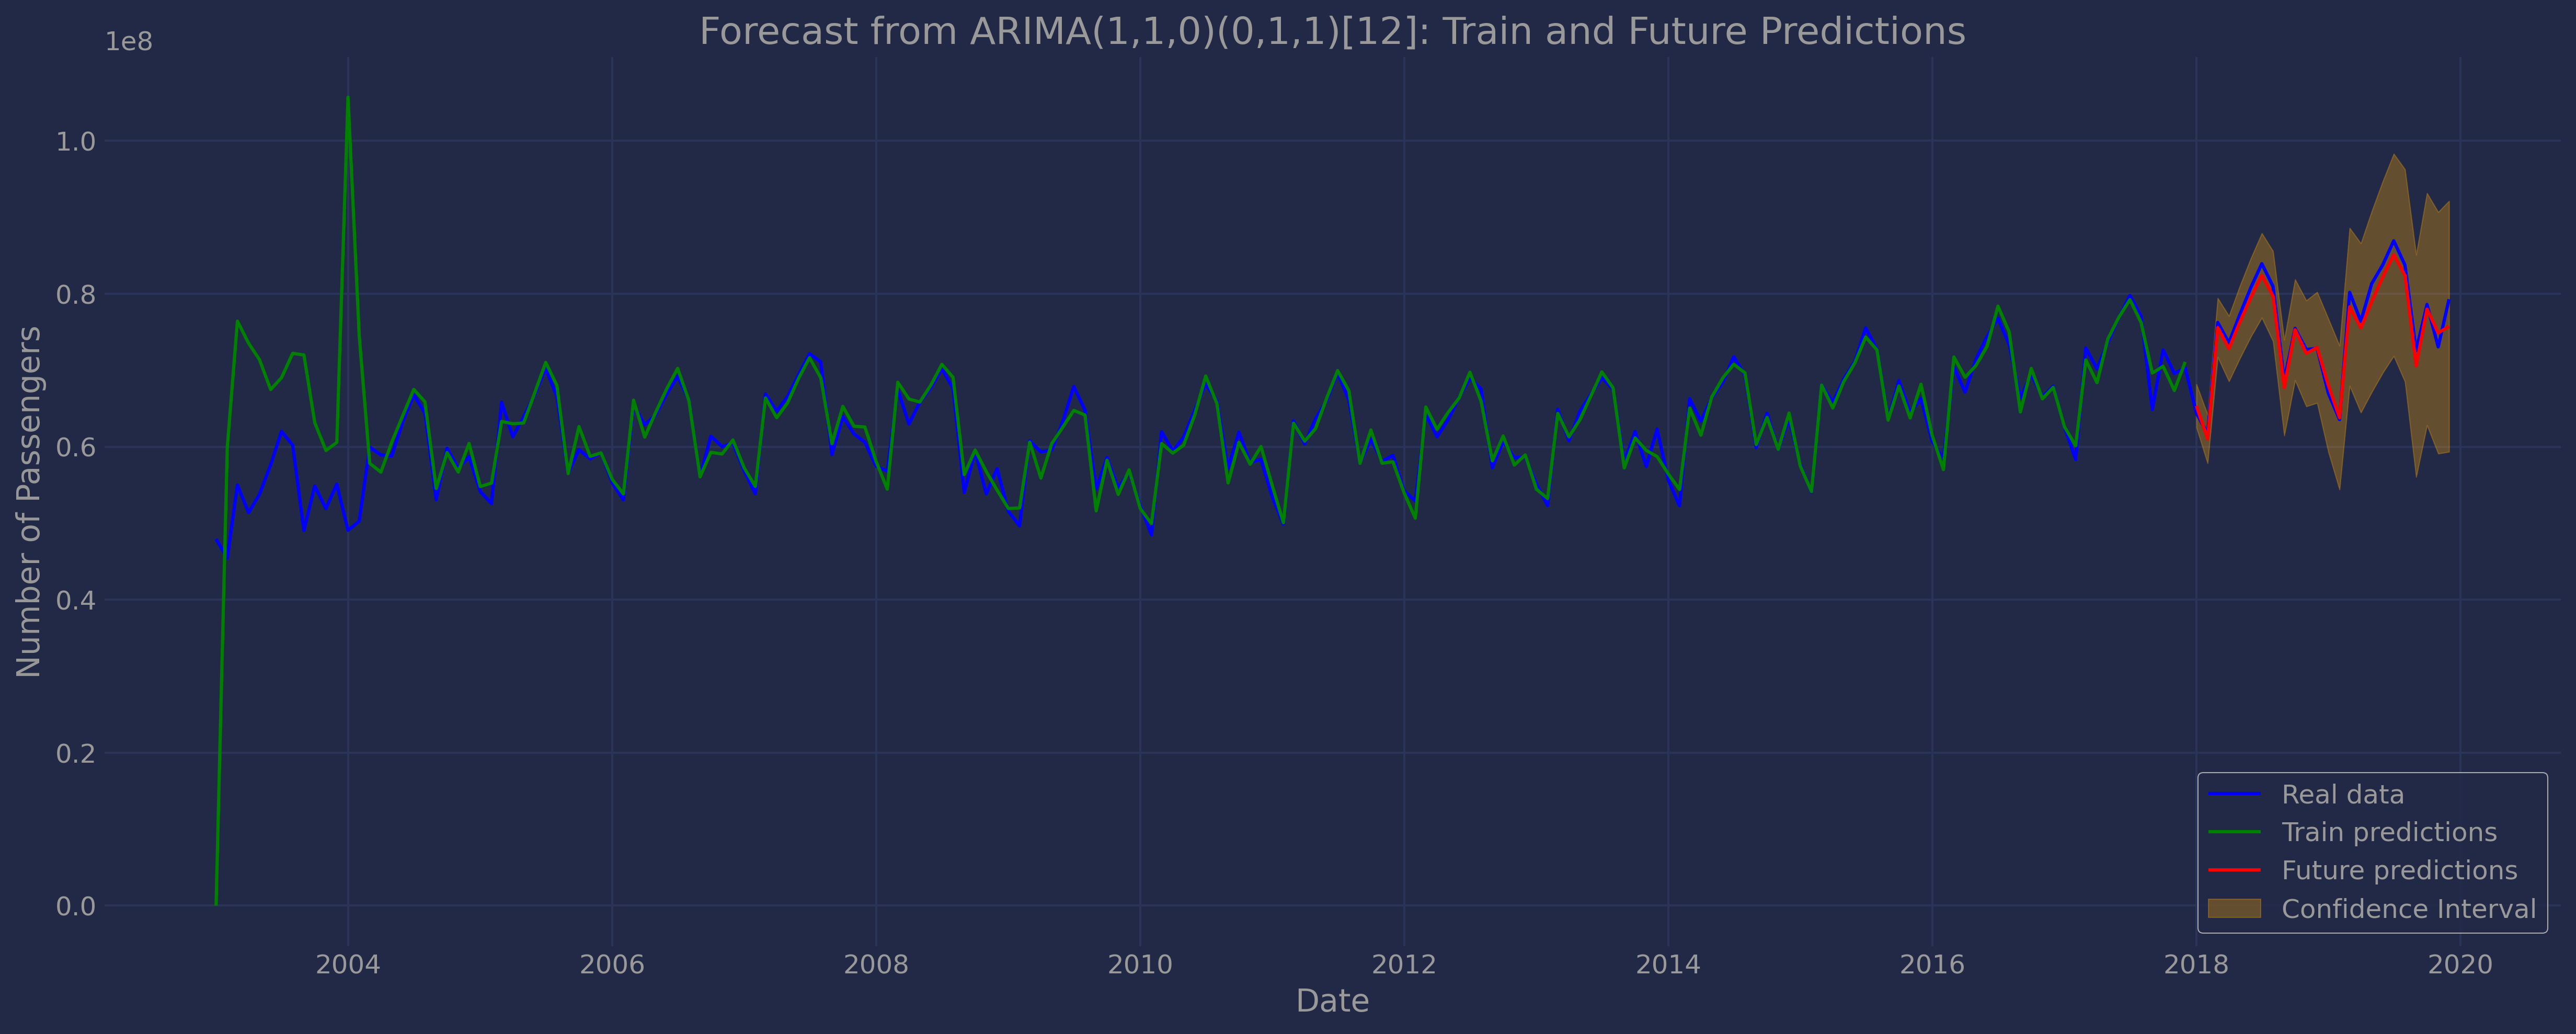
\includegraphics[width=0.8\textwidth]{pred.png}
    \caption{Predicciones del modelo SARIMA} 
    \label{fig:fig24}
\end{figure}

En primer lugar, en la Figura $~\ref{fig:fig24}$ se observa que la estacionalidad es anual, pues se repite el mismo patrón cada año. Tanto con la metodología de Box-Jenkins como con la función automática \texttt{auto\_arima}, el mejor modelo SARIMA para los datos es el modelo $ARIMA(1,1,1)_{12} \times (1,2,1)$.

En el conjunto de entrenamiento, el modelo se ajusta mejor conforme se avanza en el tiempo y se adapta adecuadamente a la tendencia que siguen los datos y a los patrones de estacionalidad. Además, se puede observar cómo las predicciones para el conjunto de prueba son precisas con respecto a los valores reales, aunque algunas predicciones están por debajo de los valores reales. No obstante, todas se encuentran dentro del intervalo de confianza al $95\%$ y este modelo tiene un error MAPE del $1,58\%$.  Además, el conjunto de entrenamiento tiene un error MAPE del $4,59\%$ como se aprecia en la Tabla $~\ref{tab:error1.1}$, por lo que no se da \textit{overfitting} ni \textit{underfitting} (~\ref{def:underfitting}).

\begin{table}[h]
\centering
\begin{tabular}{cc}
\hline
\textbf{MAPE del entrenamiento} & \textbf{MAPE del testeo} \\ \hline
4,59\% & 1,58\% \\ \hline
\end{tabular}
\caption{Errores MAPE del modelo SARIMA}
\label{tab:error1.1}
\end{table}


\subsubsection{Predicciones con el modelo SARIMA para el segundo \textit{data set}}\label{sec:37}

La función \texttt{auto\_arima} sugiere que el mejor modelo para estos datos es el modelo $ARIMA(0,1,1)_{12} \times (1,1,0)$. Sin embargo, el método Box-Jenkins lo sitúa entre los 7 posibles mejores modelos. 

\begin{figure}[h]
    \centering
    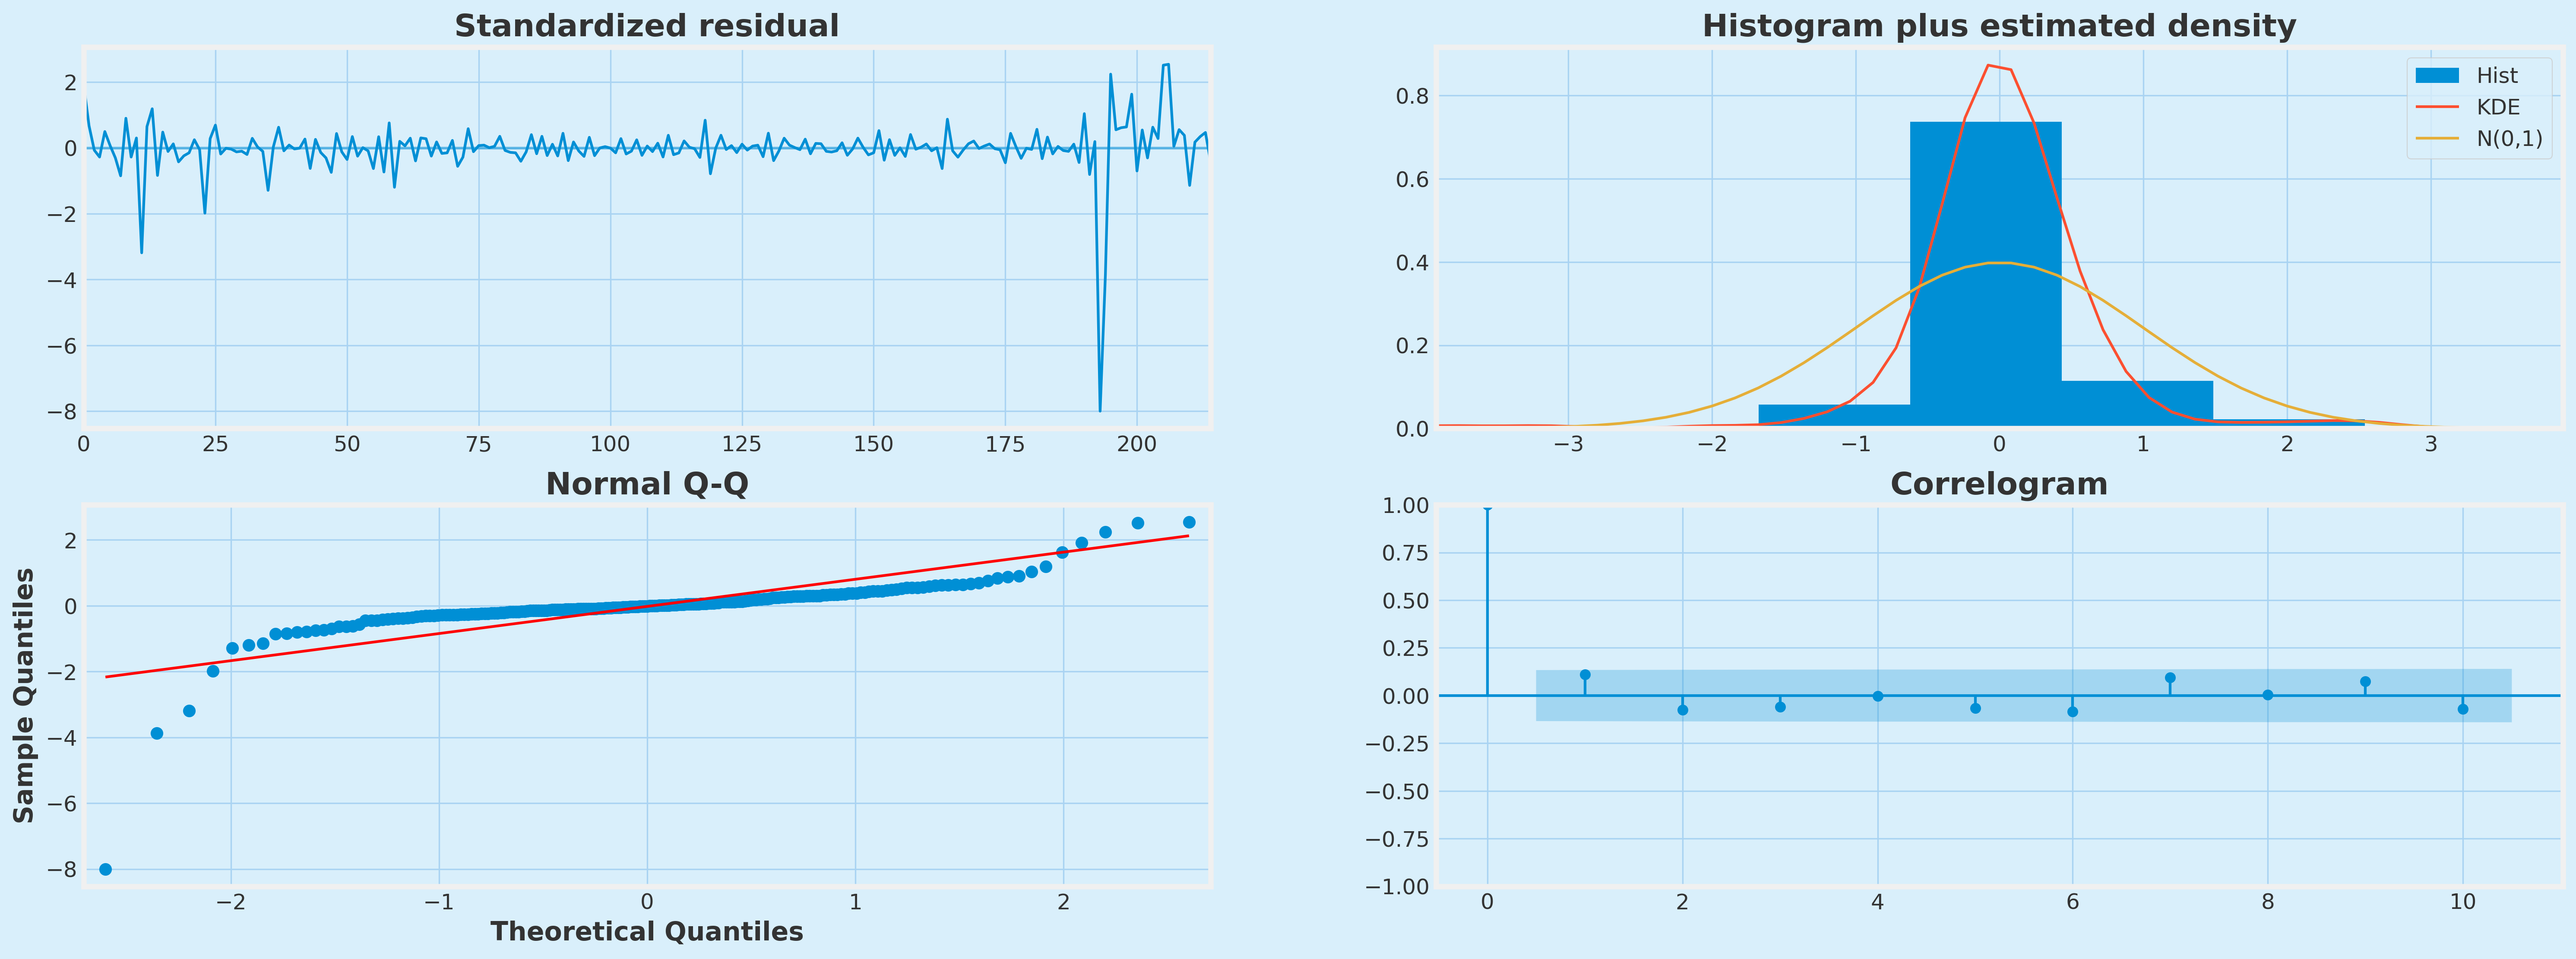
\includegraphics[width=0.6\textwidth]{residuos.png}
    \caption{Gráfica de residuos del modelo SARIMA} 
    \label{fig:fig31}
\end{figure}

En la Figura $~\ref{fig:fig31}$, se observan cuatro gráficas de los residuos del modelo SARIMA en cuestión. Se observa que los residuos estandarizados se mantienen alrededor de cero, con ciertas desviaciones al final, y el correlograma indica la ausencia de autocorrelación significativa en los residuos, por lo que se cumple el supuesto de ruido blanco. Además, el histograma y el \textit{Q-Q plot} advierten cierta leptocurtosis (mayor concentración en torno a la media y colas más pesadas que en una distribución normal estándar) en el análisis de la normalidad. Sin embargo, dado que los residuos sí que son independientes, se puede considerar el modelo apto para realizar la predicción.

\begin{figure}[h]
    \centering
    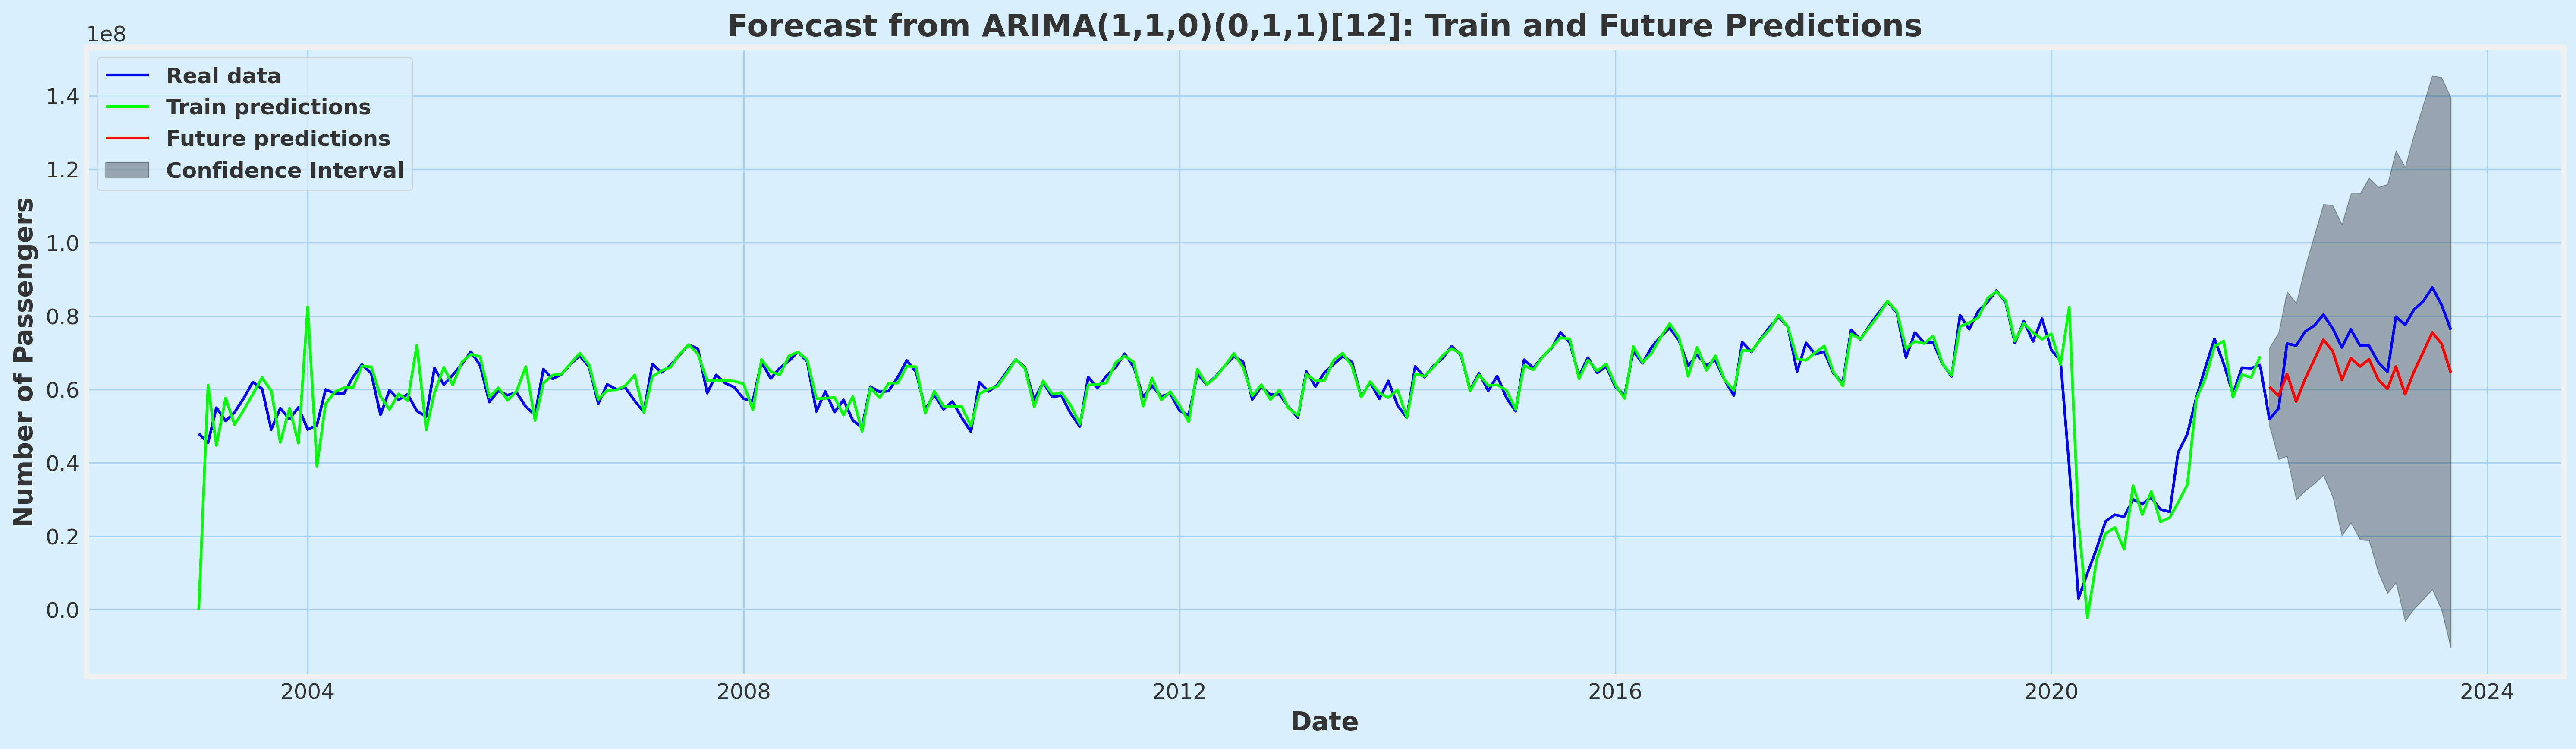
\includegraphics[width=0.8\textwidth]{pred_con.png}
    \caption{Predicciones del modelo SARIMA} 
    \label{fig:fig26}
\end{figure}

Por lo tanto, en la Figura $~\ref{fig:fig26}$ se pueden observar las predicciones del modelo. Se aprecia que, en el conjunto de entrenamiento, el modelo se adapta a la tendencia y estacionalidad de los datos, e incluso se adapta a las fluctuaciones de los meses del COVID. Sin embargo, en el conjunto de testeo, podemos ver cómo las predicciones se quedan bastante por debajo de los valores reales, por lo que el modelo no es capaz de prever la auténtica recuperación tras el COVID, de ahí que el modelo tenga un error MAPE del $12,94\%$. Además, se nota claramente que el intervalo de incertidumbre crece desmesuradamente y el conjunto de entrenamiento tiene un error MAPE del $8,65\%$,  como se aprecia en la Tabla $~\ref{tab:error1.2}$, por lo que no se da \textit{overfitting} ni \textit{underfitting}.

\begin{table}[h]
\centering
\begin{tabular}{cc}
\hline
\textbf{MAPE del entrenamiento} & \textbf{MAPE del testeo} \\ \hline
8,65\% & 12,94\% \\ \hline
\end{tabular}
\caption{Errores MAPE del modelo SARIMA}
\label{tab:error1.2}
\end{table}


\newpage
\section{Prophet}\label{sec:1}

Prophet \cite{prophet1} es uno de los modelos de predicción de series temporales más populares en la actualidad. Fue desarrollado por Facebook como software de código abierto por Sean J. Taylor y Ben Letham, y lanzado en 2017. Se destaca frente a las técnicas tradicionales por dos razones principales:

\begin{itemize}
    \item Las herramientas de predicción más automatizadas suelen ser poco flexibles y dificultan la incorporación de supuestos adicionales al modelo.
    \item Las metodologías más avanzadas requieren un alto grado de especialización, lo que implica que solo expertos en ciencia de datos pueden configurarlas correctamente.
\end{itemize}

Prophet fue diseñado específicamente para manejar las características más comunes de las series temporales en entornos empresariales, como múltiples estacionalidades fuertes, cambios de tendencia, valores atípicos y efectos de días festivos. Además, sus parámetros son intuitivos y fáciles de ajustar, lo que permite a los analistas afinar el modelo sin necesidad de comprender en profundidad sus detalles matemáticos.

Este modelo consiste en descomponer la serie temporal como suma de tres componentes, más un término de error, de la siguiente forma:

\begin{equation}
\hat{y}(t) = g(t) + s(t) + h(t) + \epsilon_t,
\end{equation}

donde:

\begin{itemize}
    \item $g(t)$ es la función de tendencia que modeliza los cambios no periódicos.
    \item $s(t)$ representa los cambios periódicos (por ejemplo, la estacionalidad semanal o anual).
    \item $h(t)$ representa los efectos vacacionales o festivos que se producen en horarios potencialmente irregulares durante uno o más días.
\end{itemize}

\subsection{Modelos de tendencia}\label{sec:2}

Se han implementado dos modelos de tendencia: un modelo no lineal de crecimiento de saturación y un modelo de tendencia lineal a trozos.

\subsubsection{Modelo no lineal de crecimiento de saturación}\label{sec:3}

Al tratar el crecimiento de la tendencia, puede resultar no ser lineal y saturarse en una cota máxima. Este tipo de crecimiento suele modelarse mediante un modelo de crecimiento logístico (en el que los datos siguen una curva sigmoide) que puede expresarse como:

\begin{equation}
g(t) = \frac{C}{1 + \exp(-k (t - m))},
\end{equation}

donde $C$ es la cota máxima de saturación, $k$ es la tasa de crecimiento y $m$ es un parámetro de compensación.

Sin embargo, este modelo presenta ciertas limitaciones. Por un lado, la cota máxima $C$ no es constante, por lo que la remplazamos por $C(t)$, que es una cota en función del tiempo. Por otro lado, la tasa de crecimiento $k$ tampoco es constante, para lo que definimos explícitamente puntos de cambio donde la tasa de crecimiento puede variar. 

Supóngase que hay $S$ puntos de cambio en los tiempos $s_j, j = 1, ..., S$. Definimos un vector de ajuste $\delta \in R^S$, donde $\delta_j$ es el cambio en la tasa que sucede en el tiempo $s_j$. Así, la tasa para cualquier tiempo $t$ es la tasa base $k$, más todos los ajustes hasta ese tiempo: $k + \sum_{j:t > s_j} \delta_j$. Esto se puede expresar de forma sencilla definiendo la función indicadora $a(t) \in \{0,1\}^S$ tal que 

\begin{equation}
a_j(t) = 
\begin{cases}
1 & \text{si } t \geq s_j \\
0 & \text{en otro caso}
\end{cases}
\end{equation}

De esta forma, la tasa de crecimiento se define como $k + a(t)^T \delta$. Una vez ajustada la tasa de crecimiento, hay que ajustar el parámetro de compensación $m$ para unir los extremos de los segmentos y que la curva sea continua. Este ajuste se obtiene como 

\begin{equation}
\gamma_j = \left( s_j - m - \sum_{l<j} \gamma_l \right) 
\left( 1 - \frac{k + \sum_{l<j} \delta_l}{k + \sum_{l \leq j} \delta_l} \right)
\end{equation}

El parámetro $m$ se puede entender como el valor inicial de la tendencia. En el instante $t = 0$, la tendencia toma el valor $m$ y, a medida que transcurre el tiempo, se ajusta en los puntos 
de cambio para reflejar las variaciones de la serie.


Así pues, el modelo lógistico queda: 

\begin{equation}
g(t) = \frac{C(t)}{1 + exp(-(k+a(t)^T \delta)(t-(m+a(t)^T \gamma)))}
\end{equation}

\subsubsection{Modelo de tendencia lineal a trozos}\label{sec:4}

Para series que no presentan un crecimiento saturado, un modelo basado en una tasa de crecimiento constante por tramos resulta una alternativa simple y eficiente. Esto permite dividir el crecimiento en distintos períodos, donde cada uno mantiene una tasa de crecimiento fija, permitiendo capturar cambios en la tendencia sin recurrir a modelos más complejos. De esto modo, nos queda el siguiente modelo de tendencia: 

\begin{equation}
g(t) = (k + a(t)^T \delta)t + (m + a(t)^T \gamma),
\end{equation}

donde, como en la sección~\ref{sec:3}, $k$ es la tasa de crecimiento, $\delta$ es la tasa ajustada, $m$ es el parámetro de compensación y $\gamma_j$ se fija como $-s_j \delta_j$ para hacer la función continua.

Se trata de un modelo lineal a trozos, lo que significa que la pendiente varía en función de $t$. Por consiguiente, a la pendiente $k$ se le suma el término  $a(t)^T \delta$.

Tanto para el modelo lineal como para el logístico, los puntos de cambio $s_j$ se pueden modificar. Normalmente, se especifica un gran número de puntos cambios (por ejemplo, uno al mes durante varios años) y se supone que $\delta_j$ sigue una distribución de Laplace con media $0$ y parámetro de escala $\tau$ ($\delta_j \sim \text{Laplace}(0, \tau))$). El parámetro $\tau$ controla la flexibilidad del modelo para alterar su tasa; es decir, conforme el valor de $\tau$ se acerca a $0$, el ajuste se reduce al crecimiento lineal (el modelo ya no tiene cambios abruptos en su tasa de crecimiento).

Además, cuando \textit{Prophet} realiza una predicción a futuro (esto es, más allá de los datos disponibles), asume que la tendencia seguirá una tasa constante y, para estimar la incertidumbre en la tendencia pronosticada, el modelo extiende la tendencia hacia el futuro. 

Cuando se estiman futuros cambios de tasa $\delta_j$, se sustituye el parámetro $\tau$ por una varianza inferida a partir de los datos. Existen dos tratamientos para estimar $\tau$: la inferencia Bayesiana con una prioridad jerárquica en $\tau$ y la estimación de máxima verisimilitud. Nos centraremos en esta última.

La estimación de máxima verosimilitud del parámetro $\tau$ se obtiene calculando la media de los valores absolutos de los cambios de tasa observados en los puntos de cambio. Esto proporciona una estimación puntual de la dispersión o variabilidad de los cambios de tasa en el modelo generativo. Así, se tiene que $\lambda = \frac{1}{S} \sum_{j=1}^{S} |\delta_j|
$. 

Entonces, los futuros puntos de cambio $s_j$ se distribuyen de manera que la frecuencia media de puntos de cambio sea la misma que la frecuencia media de puntos de cambio de los datos proporcionados:

\begin{equation}
\forall j > T, \quad 
\begin{cases} 
\delta_j = 0 & \text{con probabilidad} \quad \frac{T-S}{T}, \\
\delta_j \sim\text{Laplace}(0, \lambda) & \text{con probabilidad} \quad \frac{S}{T}.
\end{cases},
\end{equation}

donde $T$ es número total de puntos.

Por consiguiente, medimos la incertidumbre en la predicción de la tendencia considerando que en el futuro tendremos la misma frecuencia y cambios de tasa que tenemos en nuestros datos.

Por ello, la incorporación de incertidumbre en la tendencia pronosticada es relevante para cuantificar el nivel de confianza o la variabilidad en las predicciones más allá de los datos disponibles. Al pronosticar futuros cambios de tasa y tener en cuenta la incertidumbre en estos, el modelo generativo es capaz de reflejar diversos escenarios posibles y ofrecer intervalos de confianza para las predicciones futuras.

\subsection{Estacionalidad}\label{sec:5}

Las series temporales comúnmente presentan una periodicidad multitemporal. Por ejemplo, una semana laboral de cinco días puede producir efectos en una serie temporal que se repite cada semana, mientras que los horarios de vacaciones y las pausas escolares pueden producir efectos que se repiten cada año. Para ajustar y predecir estos efectos, debemos modelar la estacionalidad con funciones periódicas que dependan del tiempo. Para ello, hacemos uso de las series de Fourier ya que nos proporcionan un modelo flexible a efectos periódicos. 

Sea $P$ el periodo regular que esperamos en la serie temporal (por ejemplo, $P=365.25$ para datos anuales o $P=7$ para datos semanales), podemos aproximar los efectos estacionales a partir de la serie de Fourier 

\begin{equation}
s(t) = \sum_{n=1}^{N} \left( a_n \cos \left(\frac{2\pi n t}{P}\right) + b_n \sin \left( \frac{2\pi n t}{P}\right) \right),
\end{equation}

donde $a_n$ y $b_n$ son los coeficientes que deben estimarse a partir de los datos y $N$ define cuántos términos de la serie de Fourier se incluyen en la aproximación.

Generalmente, en una serie de Fourier los coeficientes $a_n$, $b_n$ se obtienen como

\begin{equation}
a_n = \frac{2}{P} \int_{0}^{P} y(t) \cos \left( \frac{2\pi n t}{P} \right) dt, \quad 
b_n = \frac{2}{P} \int_{0}^{P} y(t) \sin \left( \frac{2\pi n t}{P} \right) dt,
\end{equation}

donde $y(t)$ es la función que queremos aproximar.

No obstante, en la práctica estos coeficientes se estiman a partir de los datos disponibles usando regresión lineal. Para calcular los $2N$ parámetros $\beta = [ a_1, b_1, ..., a_N, b_N]^T$, construimos una matriz de vectores estacionales para cada valor de $t$ 

\begin{equation}
X(t) = \left[\cos \left(\frac{2\pi (1) t}{P}\right), \sin \left(\frac{2\pi (1) t}{P}\right), ..., \cos \left(\frac{2\pi (N) t}{P}\right), \sin \left(\frac{2\pi (N) t}{P}\right) \right]
\end{equation}

Entonces, reescribimos la componente estacional como $s(t) = X(t)\beta$. Así, para estimar los coeficientes de $\beta$, \textit{Prophet} utiliza una regresión lineal bayesiana imponiendo un prior gaussiano sobre los coeficientes; es decir, $a_n, b_n \sim \mathcal{N}(0, \sigma^2), \quad \forall n = 1, \dots, N$, para encontrar la combinación que minimiza la discrepancia entre los datos reales y las aproximaciones de la serie de Fourier. Esto actúa como un suavizado (regularización), evitando que el modelo sobreajuste a fluctuaciones aleatorias en los datos.

Además, reducir la serie a $N$ aplica un límite a la estacionalidad. Por una parte, aumentar $N$ permite detectar patrones más detallados, pero aumenta el riesgo de un sobreajuste del modelo. Por otra parte, disminuir bruscamente el valor de $N$ puede ocasionar que el modelo no detecte patrones necesarios y que se produzca un subajuste.
En general, se ha observado que utilizar $N = 10$ para la estacionalidad anual y $N = 3$ para la semanal ofrece buenos resultados en la mayoría de los casos.


\subsection{Festivos y eventos}\label{sec:6}

Hasta ahora, las componentes de Prophet desarrolladas se encuentran en la descomposición clásica de series temporales. Los días festivos y eventos especiales suelen generan grandes impactos, algo predecibles, en series temporales y, con frecuencia, no siguen un patrón periódico, por lo que sus efectos no se modelan bien con los modelos tradicionales. Por ello, \textit{Facebook} decidió añadir una nueva componente a las dos anteriores que fuera capaz de modelar estos efectos 'inesperados'.

Lo que se hace es incorporar una lista con los días festivos en el modelo, suponiendo que sus efectos son independientes. Esto simplifica el modelo al considerar cada festivo por separado, sin necesidad de modelar posibles interacciones entre ellos.

Para cada festivo $i \in \{1,..., L\}$ (donde $L$ es el número total de festivos), sea $D_i$ el conjunto de fechas pasadas y futuras para ese festivo. Añadimos una función indicadora que represente si un tiempo $t \in \mathbb{N}$ es durante el festivo $i$, y asignamos a cada festivo un parámetro $\kappa_i$ que es el cambio correspondiente en la predicción. Esto se lleva a cabo de forma similar a la estacionalidad, definiendo una matriz de regresión 

\begin{equation}
Z(t) = [1(t \in D_1),...,1(t \in D_L)]
\end{equation}

y tomando $h(t) = Z(t) \kappa$. Como en la estacionalidad, consideramos un vector previo $\kappa \sim \text{Normal}(0, \nu^2))$. 

Además, normalmente es importante incluir estos efectos alrededor de los festivos porque puede ocurrir que los efectos no se produzcan solamente en la fecha del festivo, sino que este festivo tenga consecuencias posteriores y/o anteriores. Para tener en cuenta esto, incluimos parámetros adicionales para los días que rodean el festivo, esencialmente tratando cada uno de los días en el umbral alrededor del festivo como un festivo.


\subsection{Predicciones con el modelo \textit{Prophet}}\label{sec:7}

Para finalizar la sección de \textit{Prophet}, vamos a estudiar las predicciones del modelo con los datos que se tienen. Para que el modelo pueda predecir, hay que ajustar los componentes de la ecuación y ya se estaría en condiciones de hacer cualquier predicción para cualquier valor de tiempo $t$.

Antes de empezar a predecir, cabe destacar que hay hiperparámetros \cite{prophet2} explicados en el modelo que se pueden implementar manualmente en \textit{Python}:

En cuanto a la tendencia, se puede ajustar el número de puntos de cambio con el parámetro \texttt{changepoints} si se conocen las fechas en que en que cambia la tendencia. Si se desconocen estos puntos de cambio, el modelo establece por defecto puntos de cambio en el primero 80 \% de la serie para que el modelo no esté sobreajustado (esta parámetro se puede modificar con \texttt{changepoint\_range}). Además, por defecto se establecen hasta 25 puntos de cambio, pero este valor se puede cambiar con el parámetro \texttt{n\_changepoints}.

Por otro lado, también se puede modificar el valor de $\tau$ (parámetro de escala de la distribución de Laplace para la tasa $\delta$) con \texttt{changepoint\_prior\_scale}, que por defecto es 0,05. Un valor bajo hace que la tendecia del modelo sea más rígida, llegando al \textit{underfitting} si este valor es demasiado bajo; mientras que un valor alto ayuda a que la tendencia sea más flexible, llegando a caer en el \textit{overfitting} si es demasiado alto.

Para obtener los parámetros $k$ y $m$, lo que hace \textit{Prophet} internamente es combinarlos hasta obtener el menor error cuadrático medio para el conjunto de entrenamiento.

Por último, Prophet permite ajustar el crecimiento lineal o logístico con el parámetro \texttt{growth}, siendo como valor predeterminado el crecimiento lineal.

En lo que respecta a la implementación de la estacionalidad, se puede ajustar el parámetro $\beta$ del modelo con \texttt{seasonality\_prior\_scale}, que por defecto es 10. Un valor alto permite que el modelo puede ajustarse mejor a los patrones estacionales de los datos y un valor más bajo da como resultado un modelo más uniforme y menos reactivo a los patrones estacionales.

Además, se puede concretar el tipo de estacionalidad (aditiva o multiplicativa) con el comando \texttt{seasonality\_mode}, que por defecto es aditiva. En el caso en que sea multiplicativa, también siguen un modelo multiplicativo los festivos y eventos, pero se puede especificar el tipo de modelo de cada componente con el parámetro \texttt{mode}. Tambíen se puede ajustar el parámetro $N$ con el parámetro \texttt{yearly\_seasonality}.

Por último, para la implementación de los festivos, se pueden añadir como una lista de fechas con el parámetro \texttt{holidays} y el parámetro $\kappa$ del modelo se puede ajustar con \texttt{holidays\_prior\_scale}, cuyo valor predeterminado es 10. Un valor mayor hace que el modelo se ajuste mejor a los efectos de los días festivos, mientras que un valor inferior limita la influencia de estos días festivos en las predicciones.

\subsubsection{Predicciones con el modelo \textit{Prophet} para el primer \textit{data set}}\label{sec:8}

\begin{figure}[h]
    \centering
    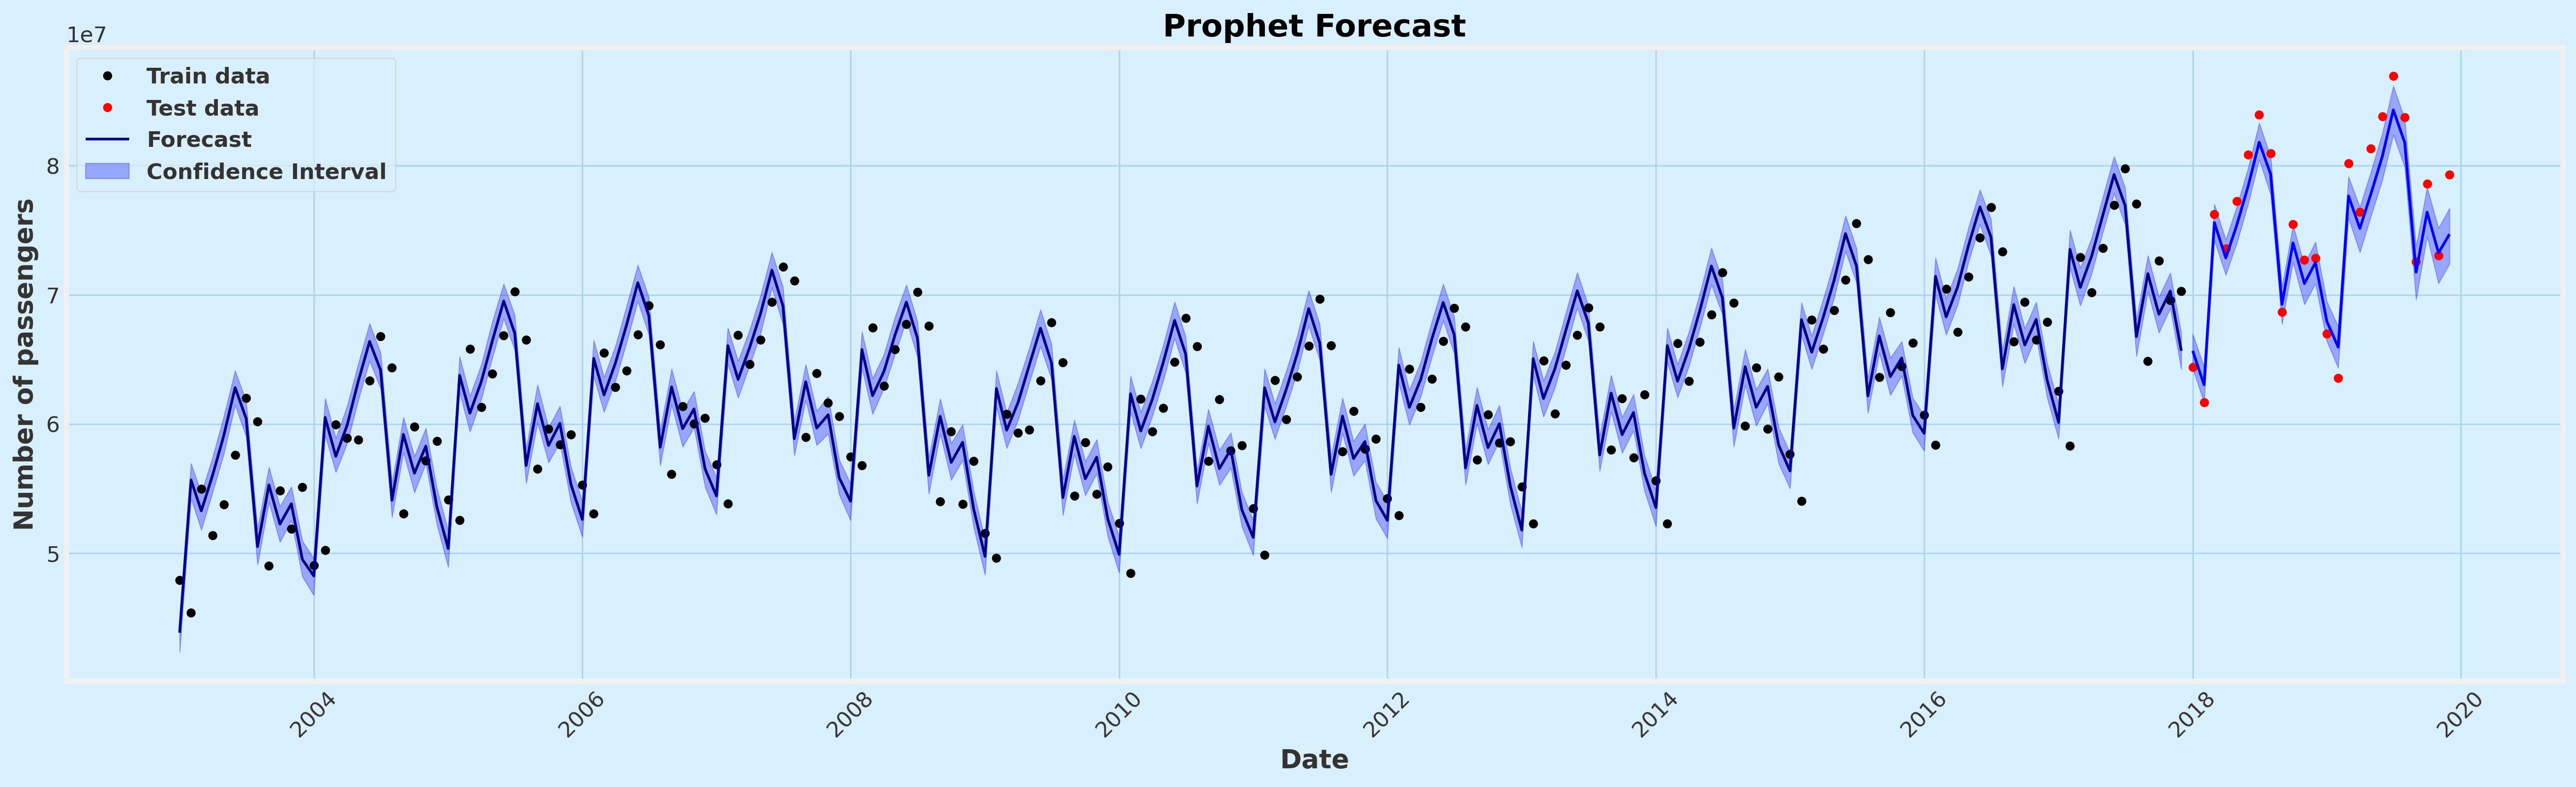
\includegraphics[width=0.8 \textwidth]{forecast_plot.png}
    \caption{Predicciones del modelo Prophet con parámetros por defecto} 
    \label{fig:fig1}
\end{figure}

Para este conjunto de datos, como no aparecen los años del COVID, se considera que no hay festividades. Para una primera aproximación, se realizan las predicciones con los parámetros por defecto, Figura $~\ref{fig:fig1}$.

%\begin{figure}[h]
%    \centering
%    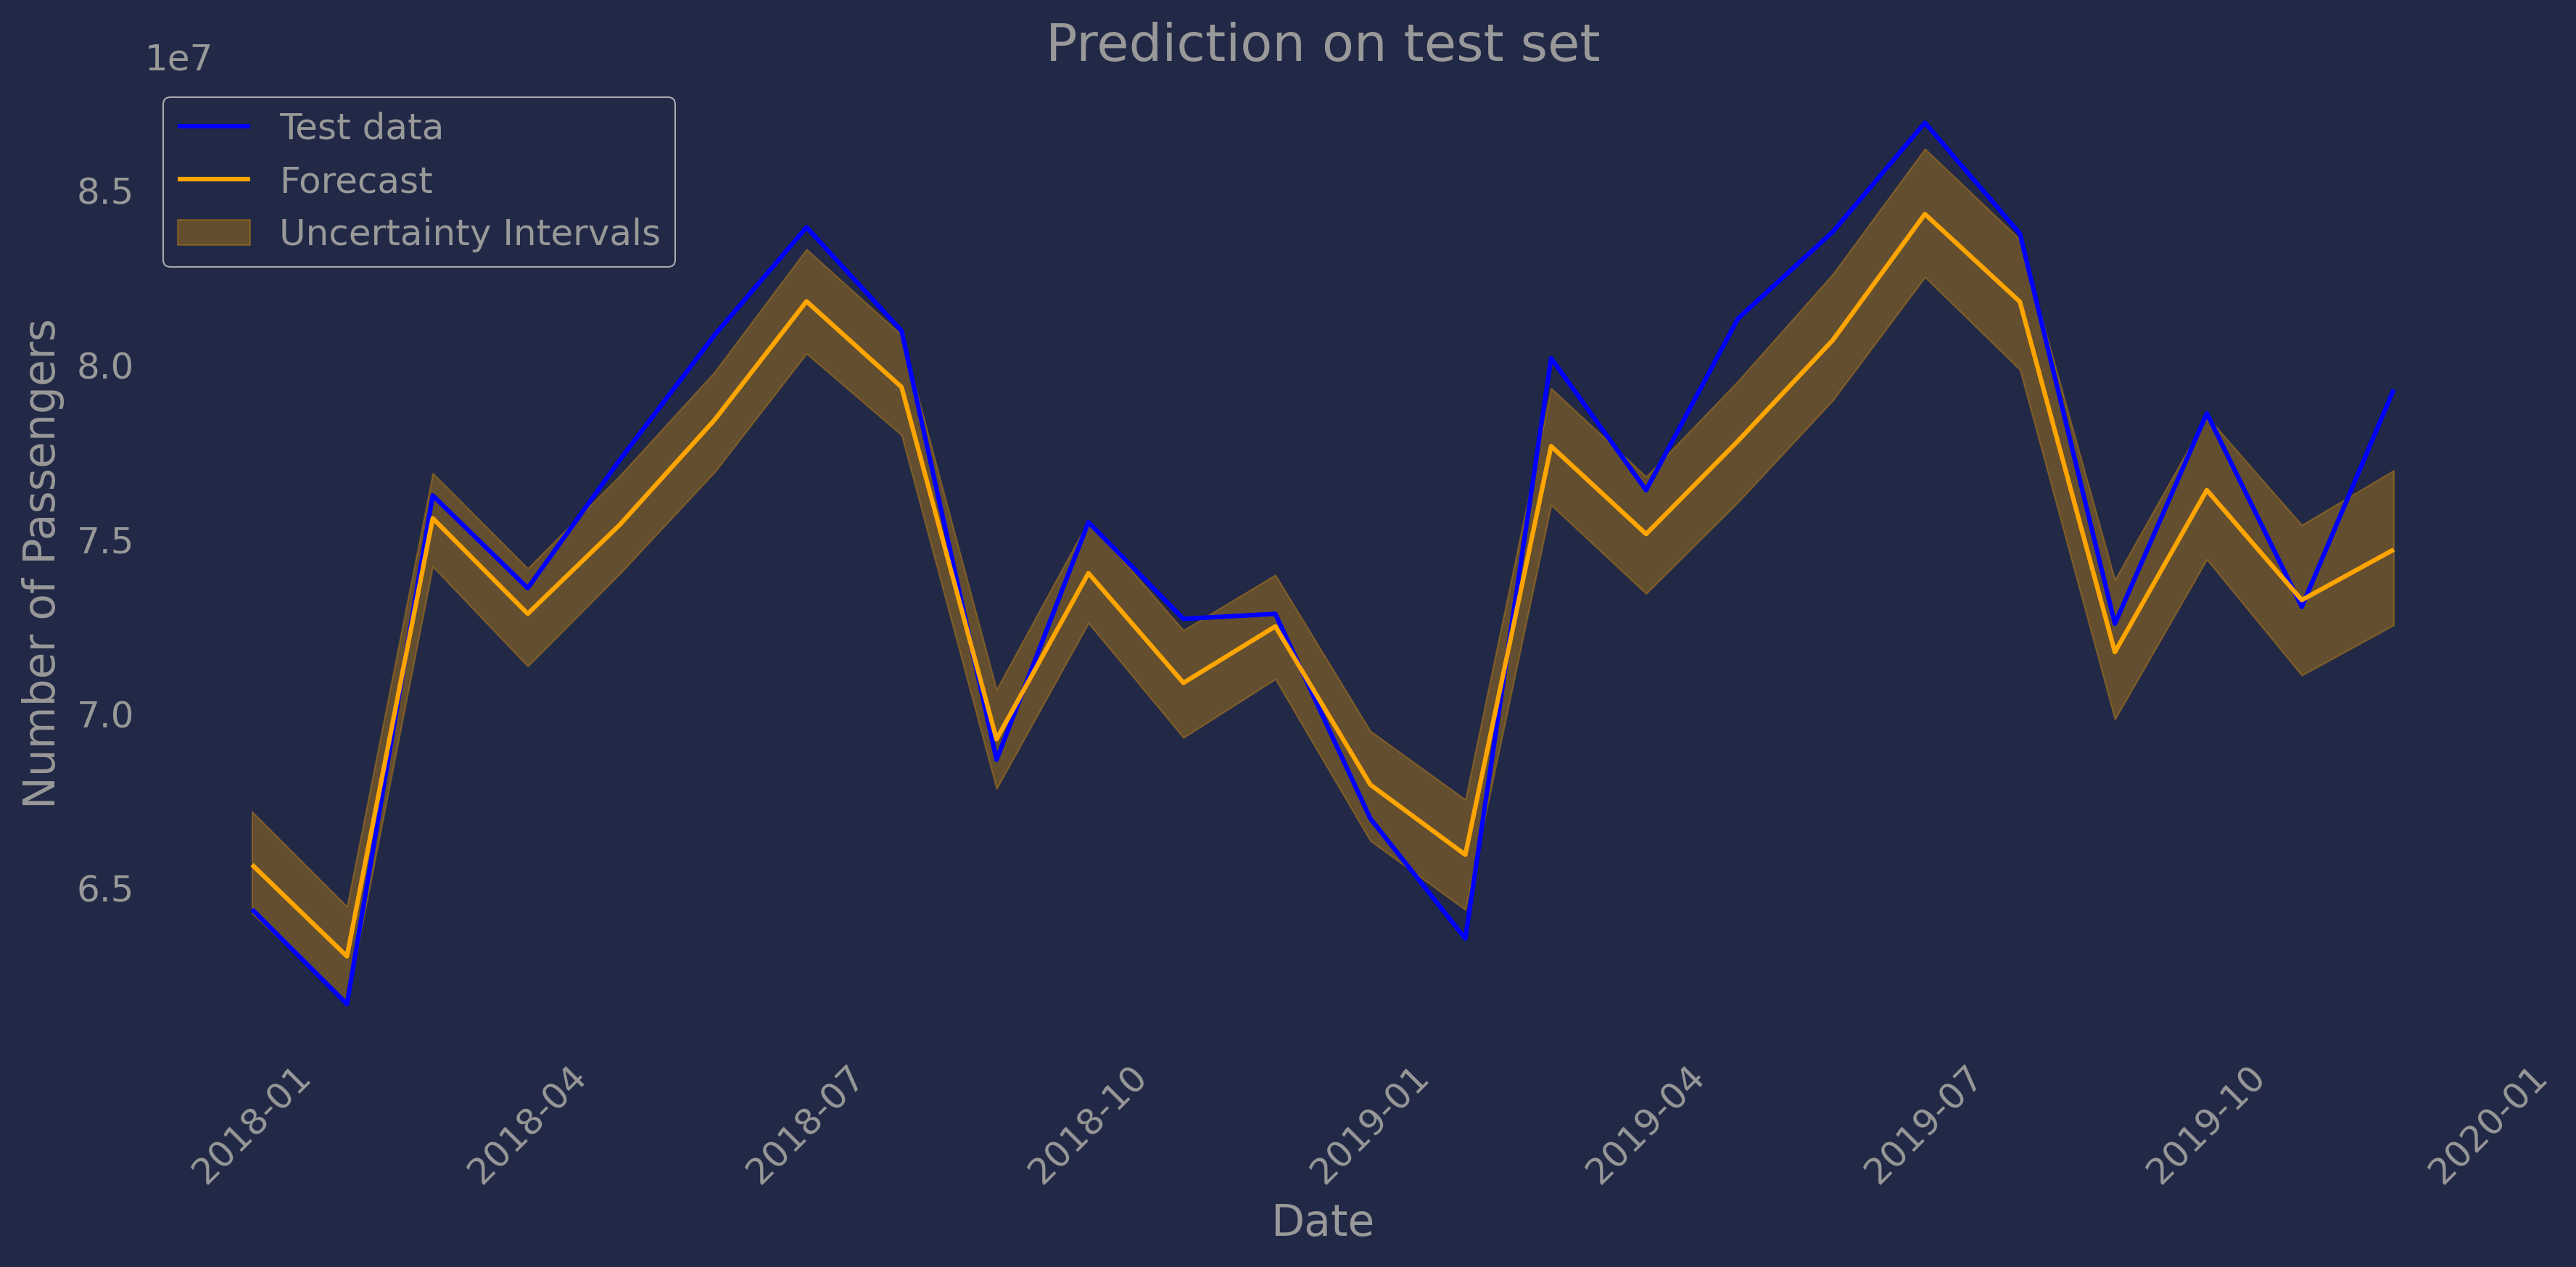
\includegraphics[width=0.8 \textwidth]{predictions_on_test_set.png}
%    \caption{Predicciones del modelo Prophet con parámetros por defecto para los años 2018-2019} 
%    \label{fig:fig2}
%\end{figure}


Al predecir para los años 2018-2019, años con los que el modelo no ha sido entrenado, se puede ver que el modelo se ajusta a ellos. En general, el modelo sigue bien la tendencia general de los datos, capturando los patrones que siguen, aunque algunos datos reales no caen dentro de los intervalos de confianza. Este modelo tiene un error MAPE del $2,30\%$.

A continuación, se implementa de nuevo el modelo pero escogiendo los mejores parámetros a partir de combinaciones de parámetros específicos, varios de los mencionados anteriormente. Se proponen varias posibilidades para cada parámetro y se generan todas las combinaciones de posibles hiperparámetros. Entonces, para cada combinación, se ajusta un modelo Prophet sobre los datos de entrenamiento y se evalúa con validación cruzada temporal (~\ref{def:val}). Finalmente, se elige la mejor combinación de hiperparámetros como aquella que minimiza el error RMSE, que consiste en la raíz cuadrada del error MSE. Estos parámetros son: 

\begin{table}[ht] 
\centering
\begin{tabular}{rrr} 
  \hline
 \texttt{changepoint\_prior\_scale} & \texttt{changepoint\_range} & \texttt{seasonality\_prior\_scale} \\ 
  \hline
0.5 & 0.8 & 1.0 \\ 
   \hline
\end{tabular}
\end{table}

\begin{table}[ht] 
\centering
\begin{tabular}{rrrr} 
  \hline
 \texttt{holidays\_prior\_scale} & \texttt{seasonality\_mode} & \texttt{growth} & \texttt{yearly\_seasonality} \\ 
  \hline
0.05 & multiplicative & logistic & 20 \\ 
   \hline
\end{tabular}
\caption{Mejores parámetros escogidos} \label{tab:01}
\end{table}

\begin{figure}[h]
    \centering
    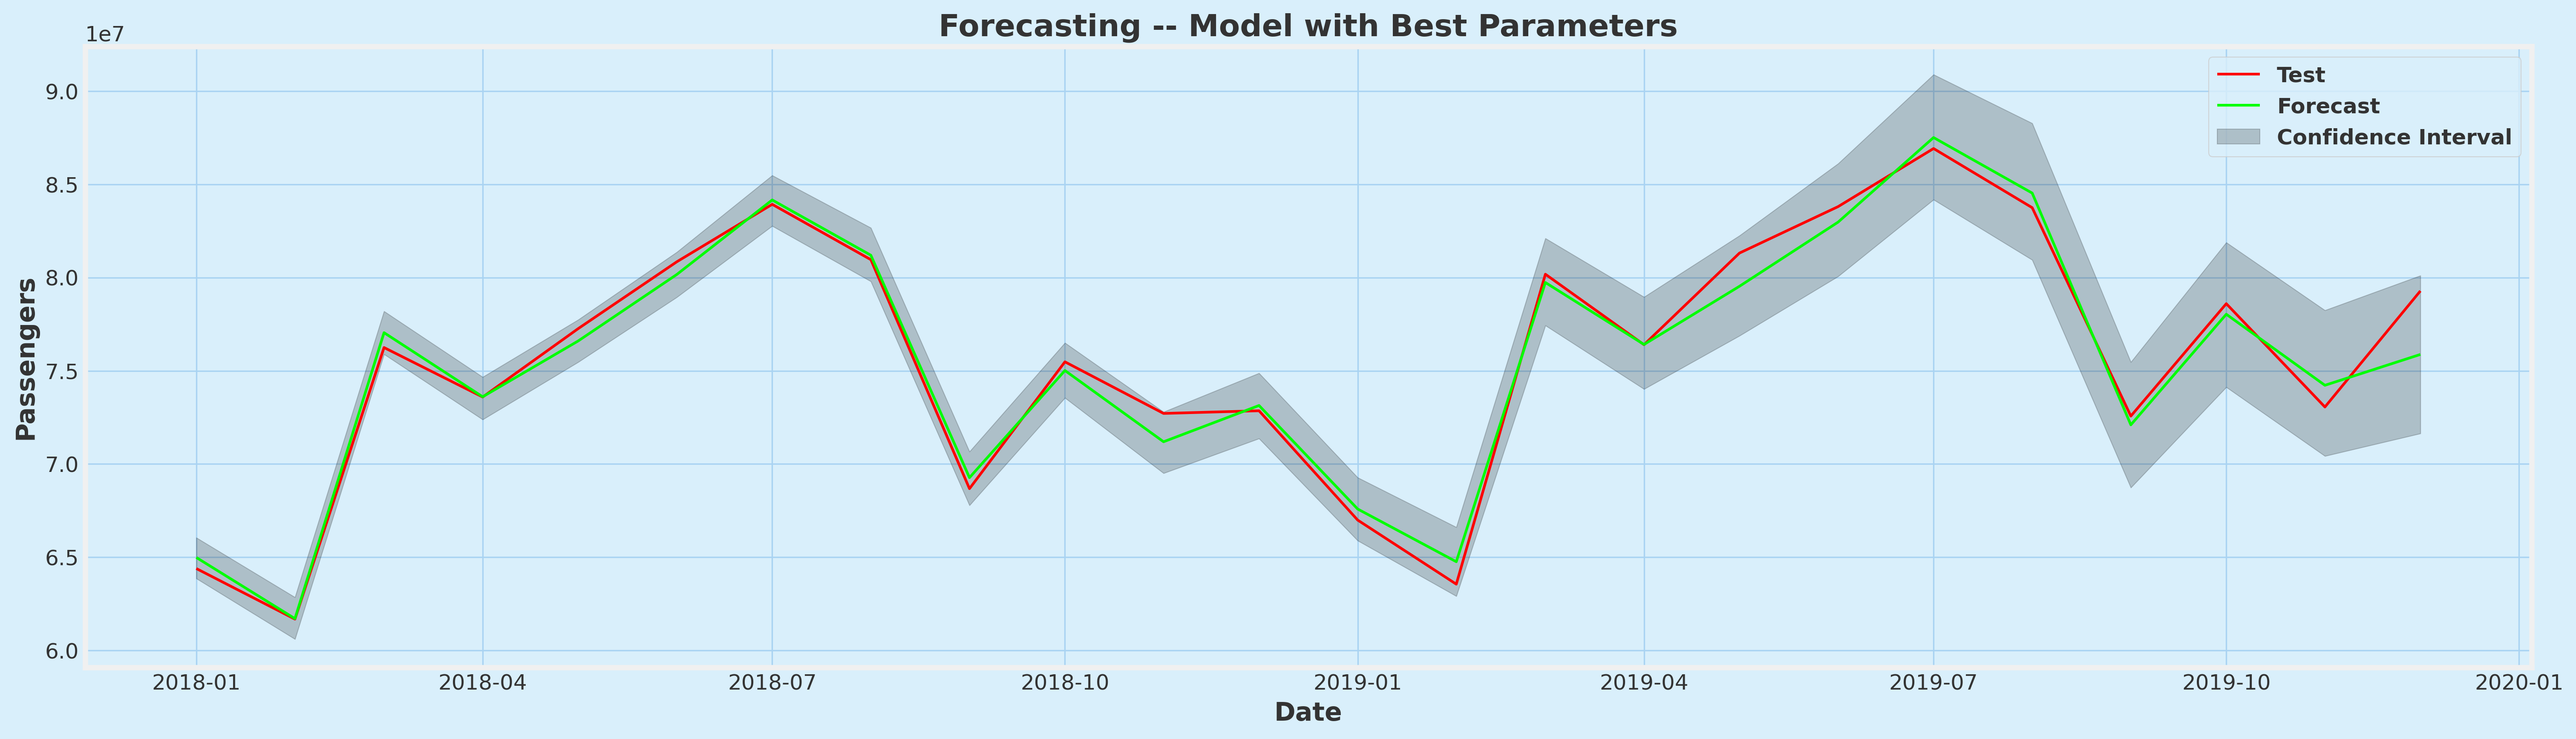
\includegraphics[width=0.8 \textwidth]{predictions_on_test_set_best_params.png}
    \caption{Predicciones del modelo Prophet con los mejores parámetros para los años 2018-2019} 
    \label{fig:fig3}
\end{figure}

Observando las prediciones para los años 2018-2019 con el nuevo modelo, Figura $~\ref{fig:fig3}$, se ve que ahora el modelo se adapta incluso mejor a los datos y que las predicciones son más exactas. También, todos los valores reales caen dentro del intervalo de confianza y este modelo tiene un error MAPE del $0.99\%$.

\begin{table}[h]
\centering
\begin{tabular}{ccc}
\hline
\textbf{Modelo} & \textbf{MAPE del entrenamiento} & \textbf{MAPE del testeo} \\ \hline
\text{Con valores por defecto} & 7,40\% & 2,30\% \\ \hline
\text{Con los mejores parámetros} & 7,37\% & 0,99\% \\ \hline
\end{tabular}
\caption{Errores MAPE del modelo Prophet}
\label{tab:error2.1}
\end{table}

Así, comparando los errores MAPE para ambos modelos en la Tabla $~\ref{tab:error2.1}$, se aprecia que el segundo modelo es mejor que el primero al tener menor error MAPE tanto en el entrenamiento como en el testeo, y ninguno cae en \textit{overfitting} ni \textit{underfitting}. Se nota que para este conjunto de datos, lo mejor es el crecimiento logístico y la estacionalidad multiplicativa.

\begin{figure}[h]
    \centering
    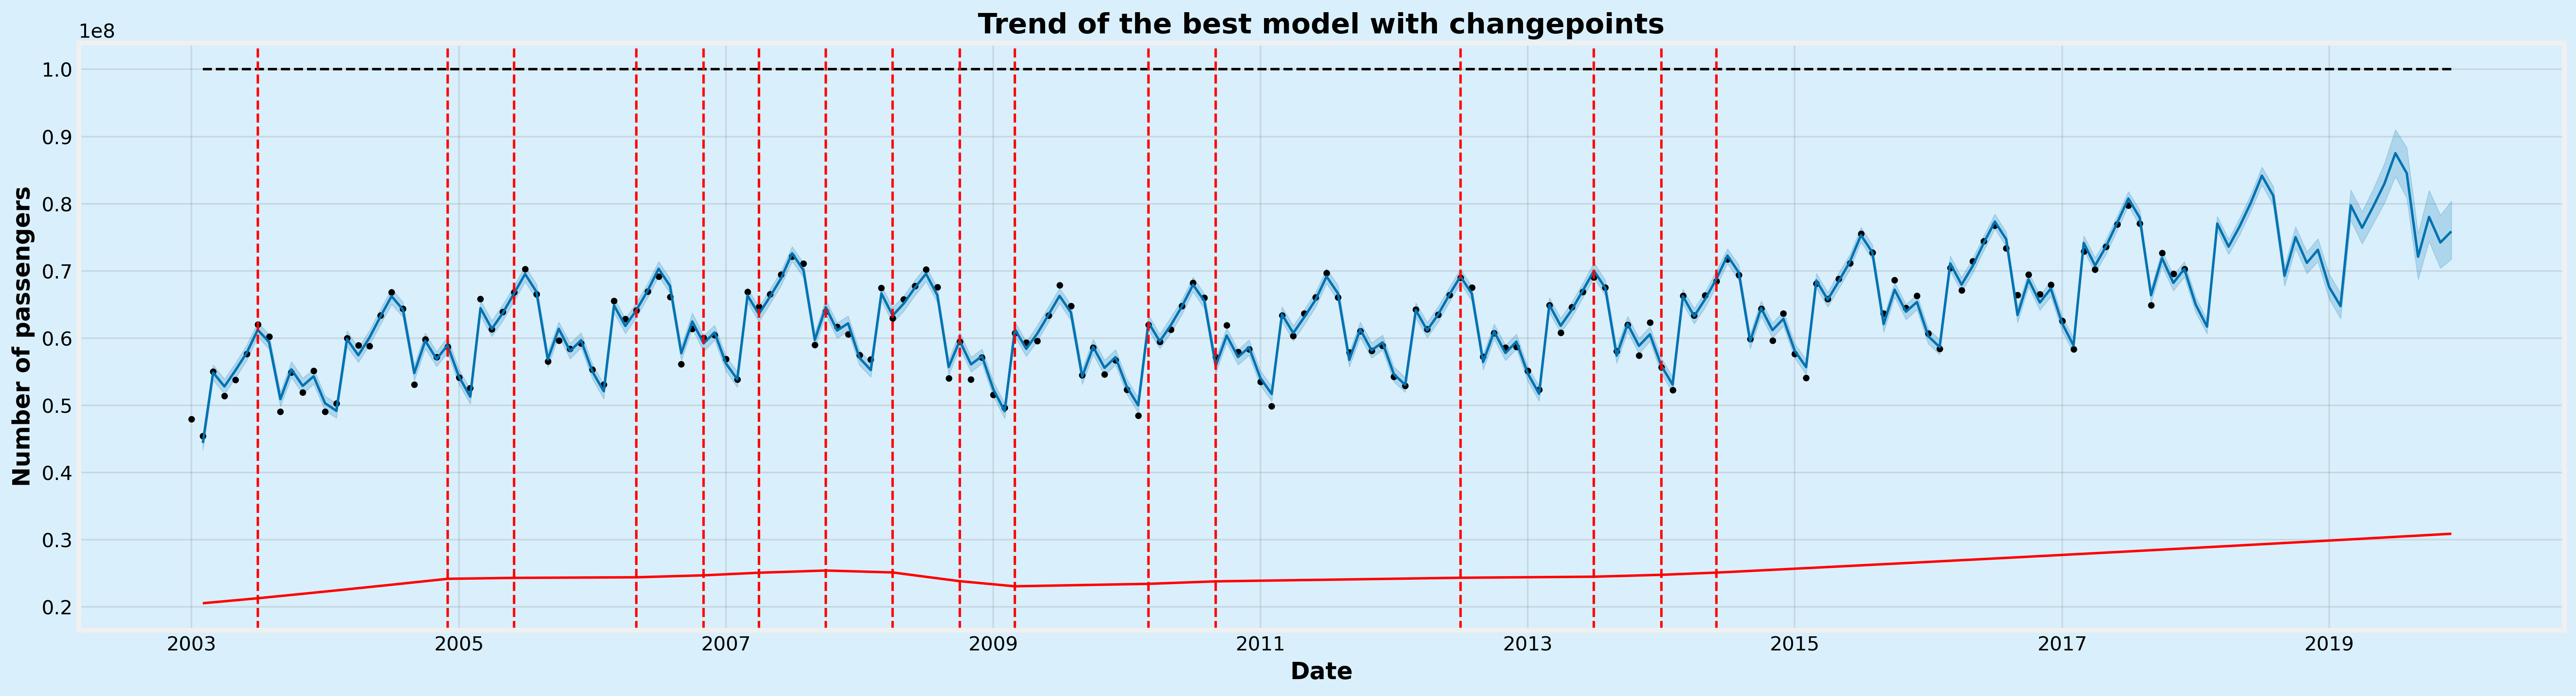
\includegraphics[width=0.8 \textwidth]{changepoints.png}
    \caption{Puntos de cambio para el mejor modelo} 
    \label{fig:fig4}
\end{figure}

Además, para este modelo, se observa en la Figura $~\ref{fig:fig4}$ que se han tomado 16 puntos de cambio, pero no de forma demasiado abrupta; es decir, la tendencia no varía demasiado con el tiempo e incluso parece que la tendencia podría modelarse con dos líneas rectas. 

\subsubsection{Predicciones con el modelo \textit{Prophet} para el segundo \textit{data set}}\label{sec:9}

\begin{figure}[h]
    \centering
    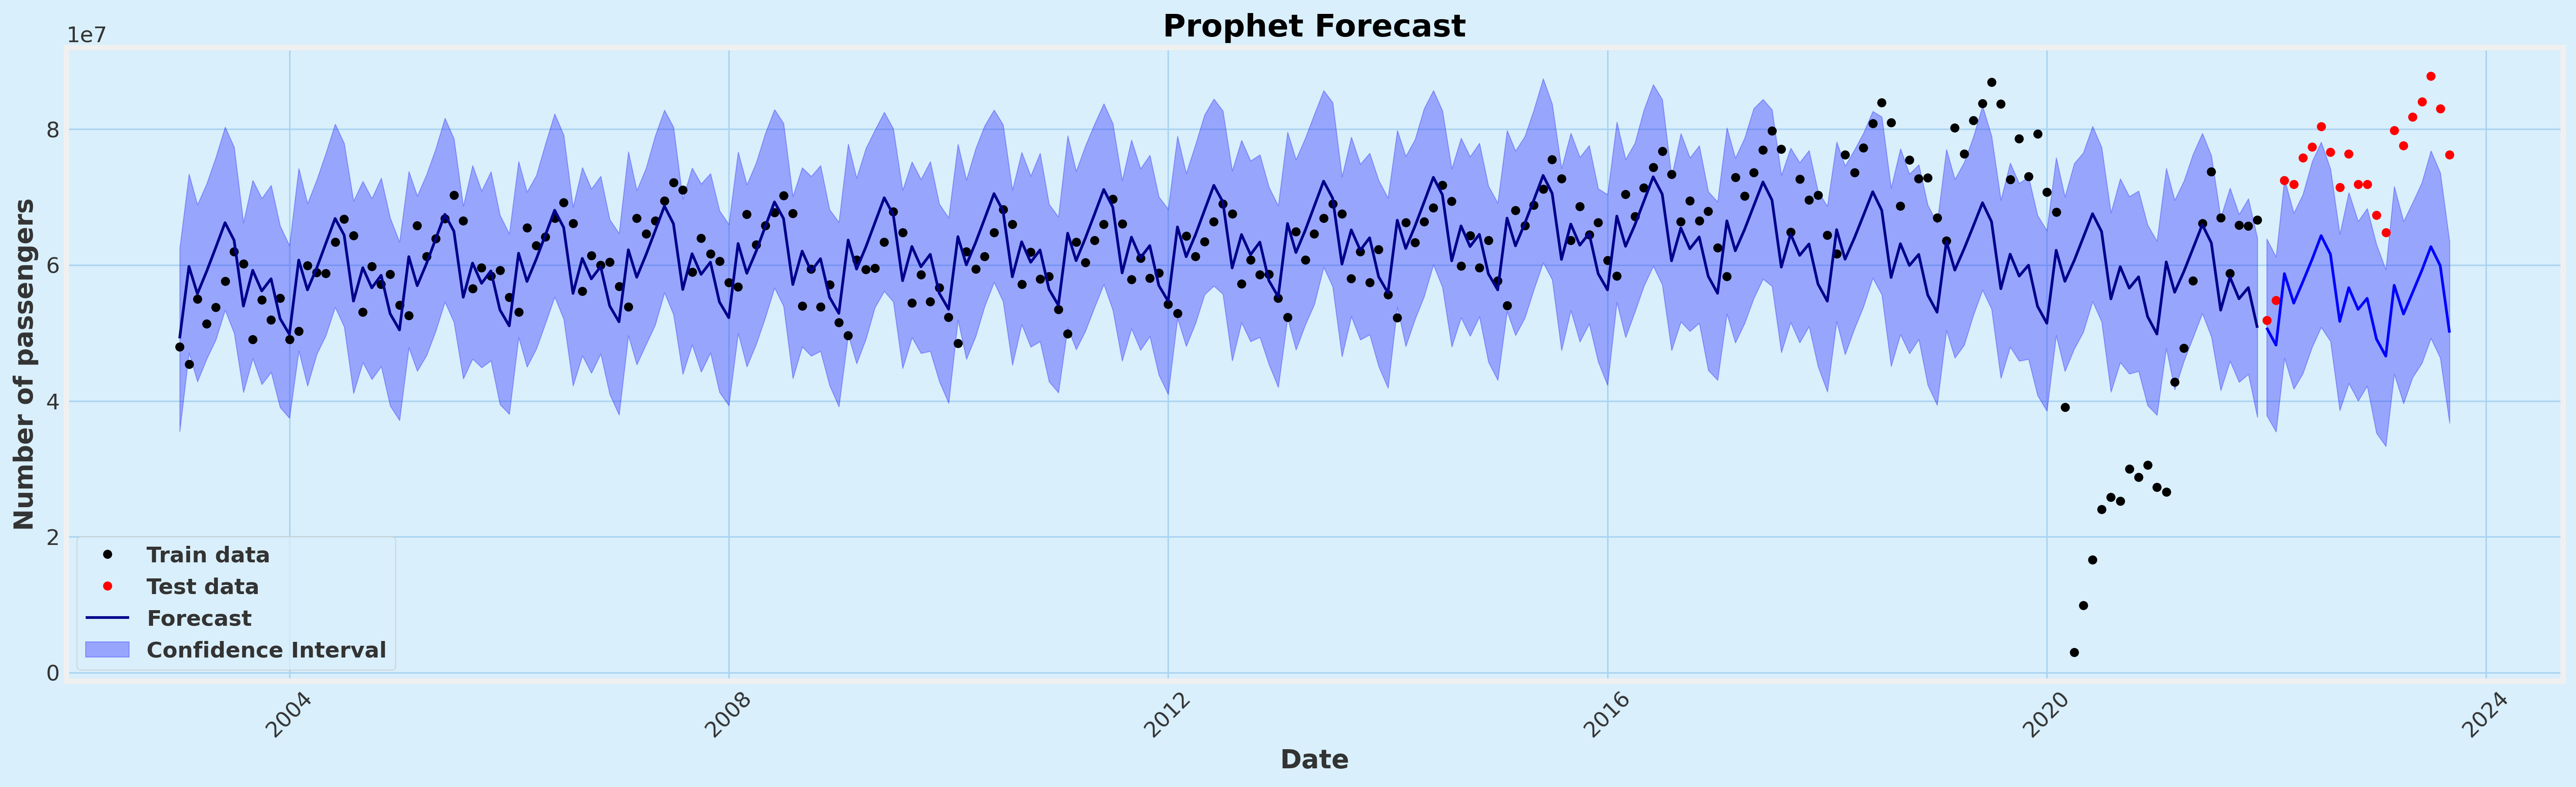
\includegraphics[width=0.8 \textwidth]{Prophet_forecast.png}
    \caption{Predicciones del modelo Prophet con parámetros por defecto} 
    \label{fig:fig5}
\end{figure}

Para este \textit{data set}, se parte proponiendo un modelo con valores por defecto sin añadir festivos. En la Figura $~\ref{fig:fig5}$, se observan las predicciones del modelo y se puede notar que no es capaz de capturar el repentino descenso en el número de pasajeros para las aerolíneas estadounidenses durante el COVID.

%\begin{figure}[h]
%    \centering
%    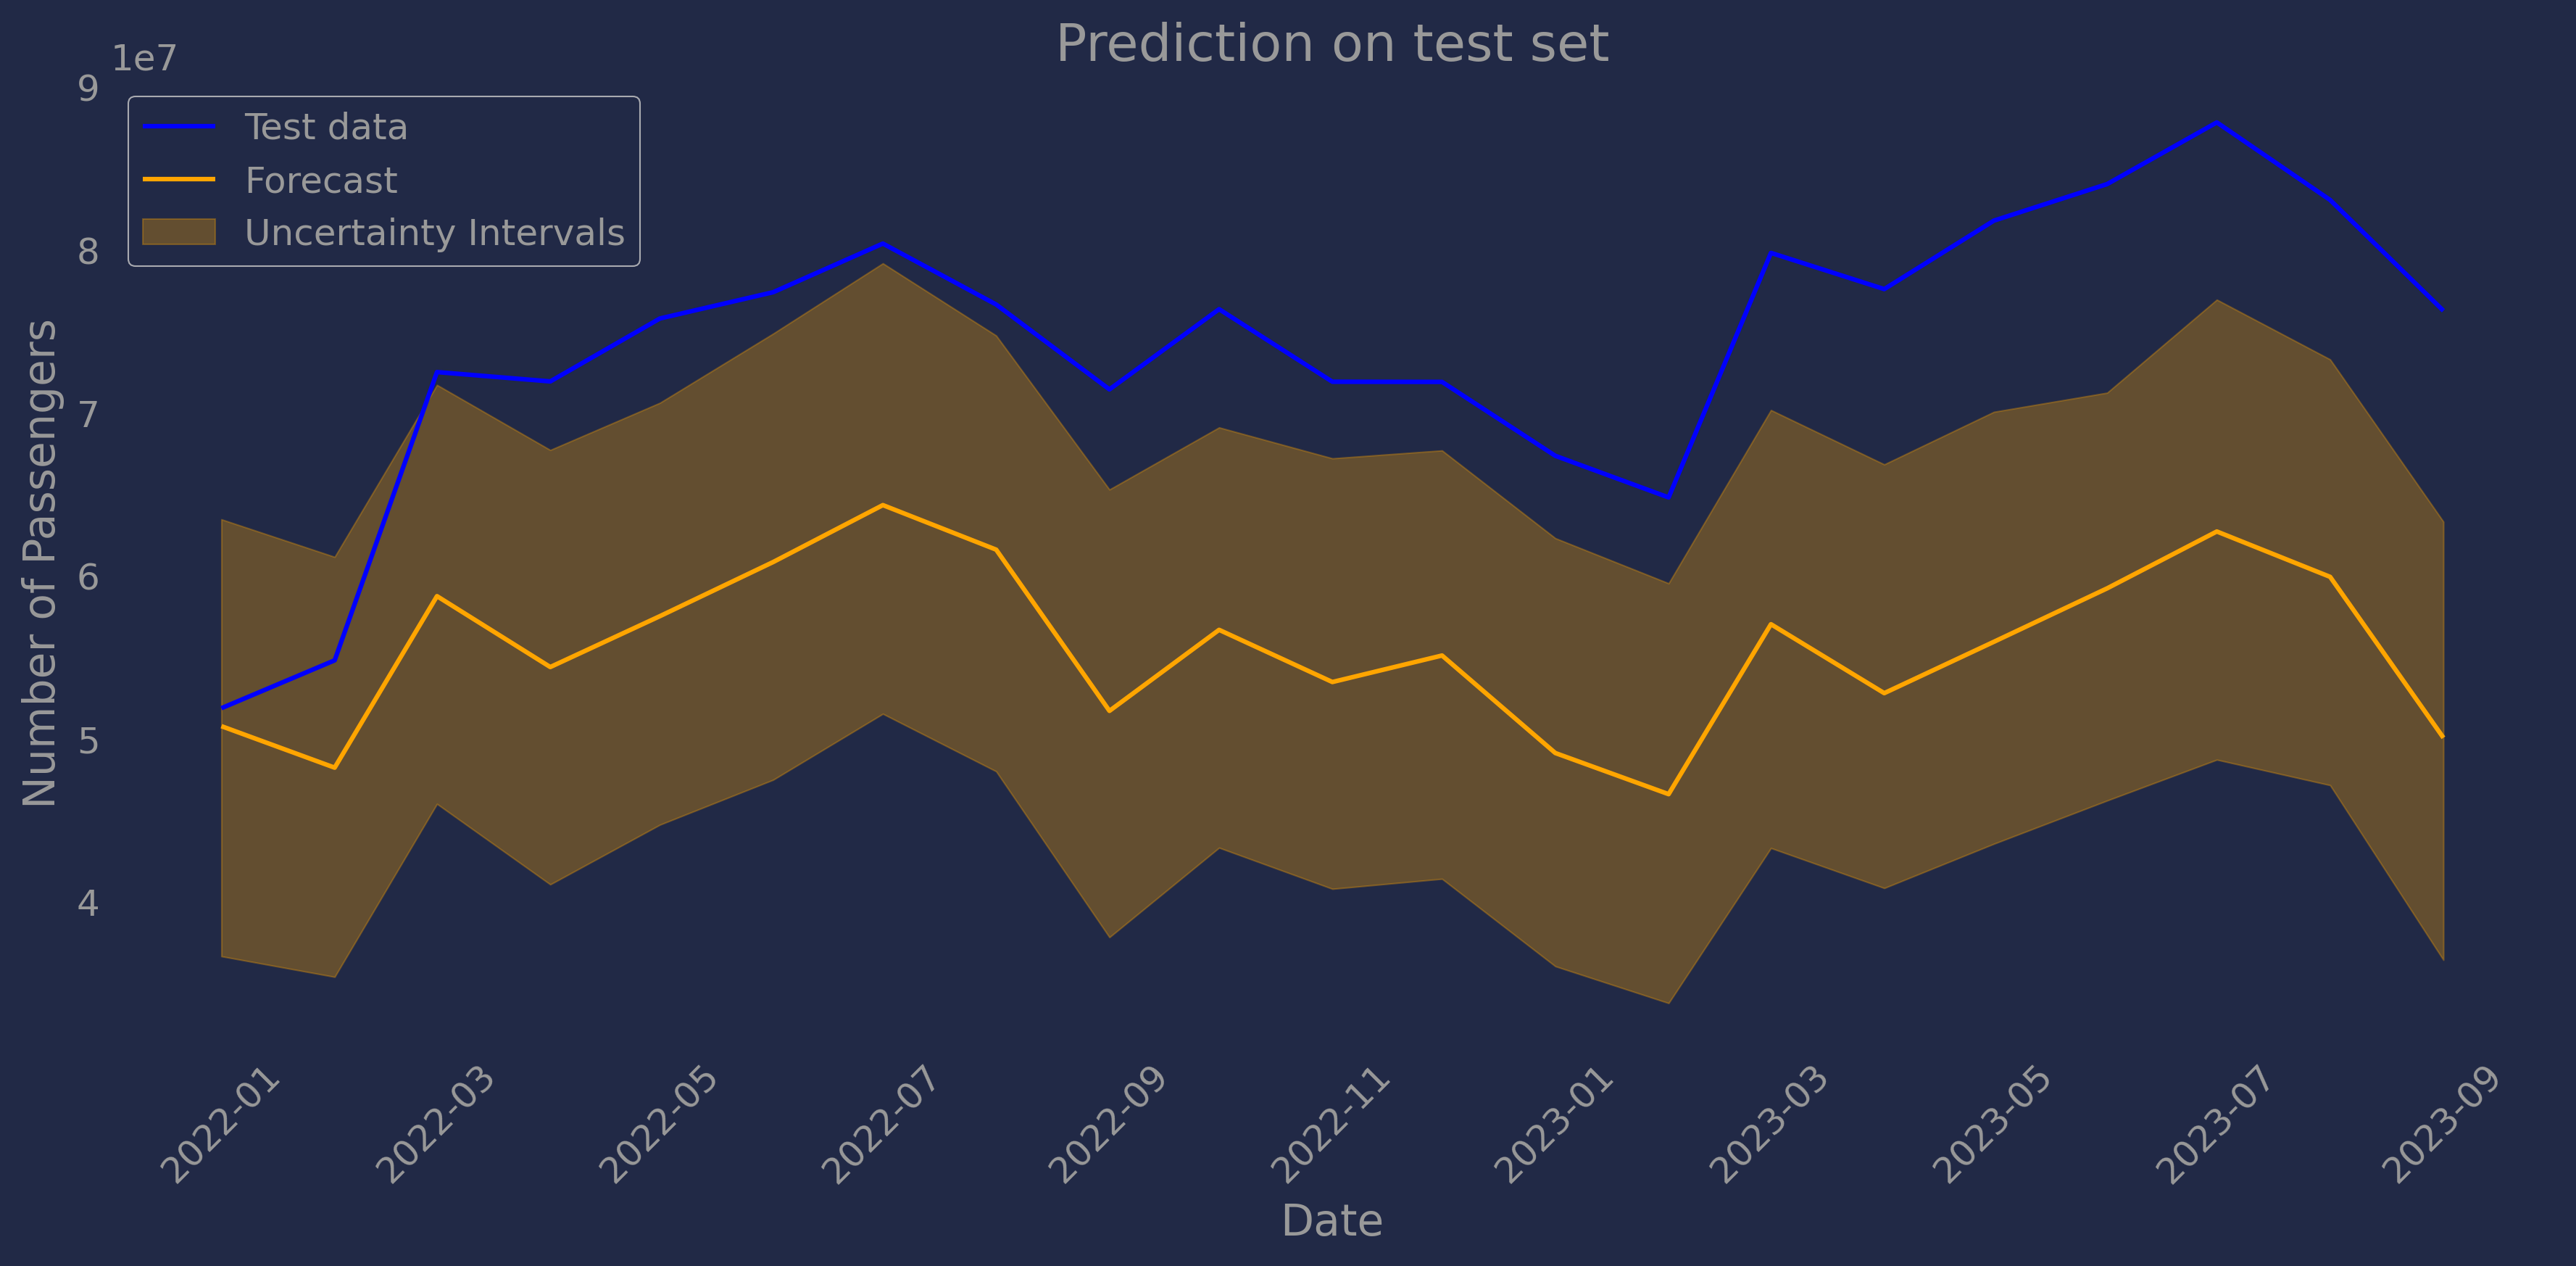
\includegraphics[width=0.8 \textwidth]{pred_test.png}
%    \caption{Predicciones del modelo Prophet con parámetros por defecto para los años 2022-2023} 
%    \label{fig:fig6}
%\end{figure}

Además, se observa que las predicciones para los años 2022 y 2023 no son precisas. De hecho, los valores reales se encuentran fuera del intervalo de confianza y todos los valores predichos son menores que los valores reales, por lo que el modelo no se adapta a la recuperación de la normalidad tras el COVID. Por otro lado, este modelo tiene un error MAPE del $24,41\%$.

\begin{figure}[h]
    \centering
    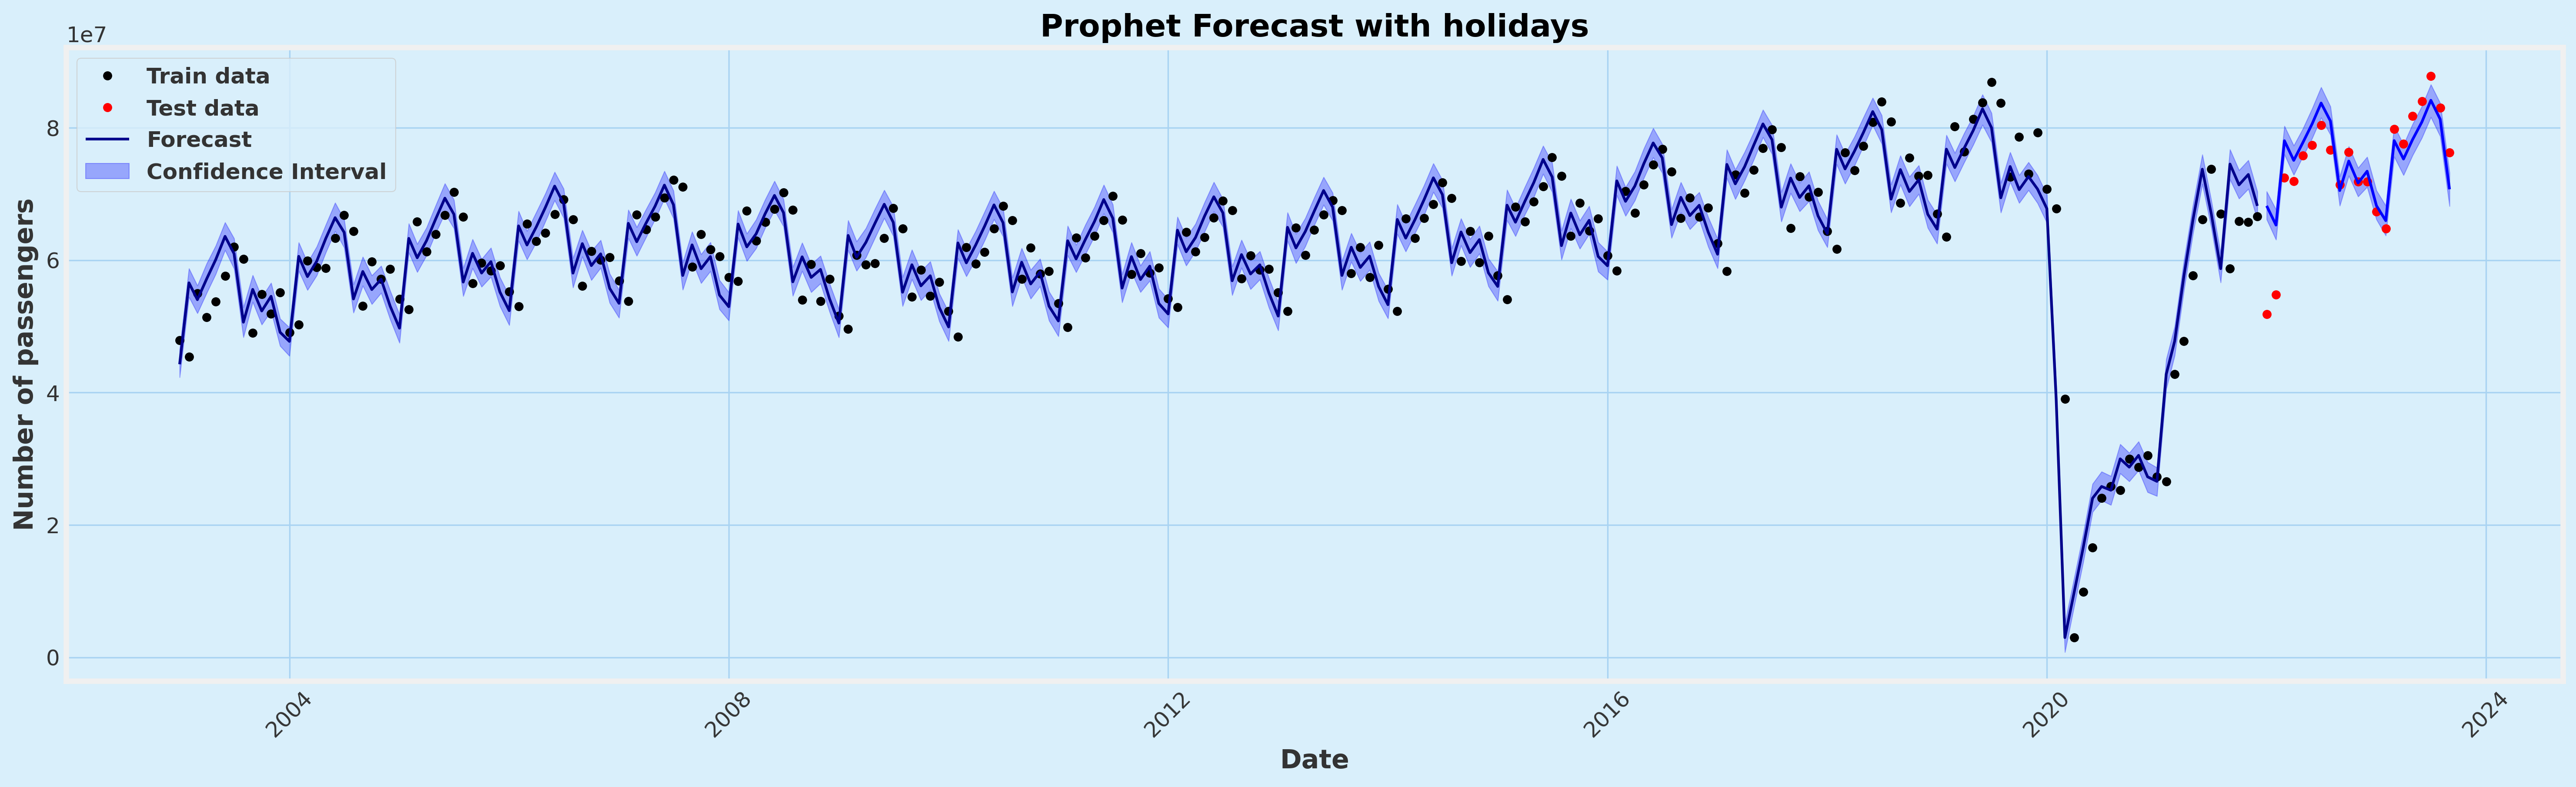
\includegraphics[width=0.8 \textwidth]{Prophet_hol.png}
    \caption{Predicciones del modelo Prophet con festivos y parámetros por defecto} 
    \label{fig:fig7}
\end{figure}

Para intentar mejorar este modelo, se propone el mismo pero añadiéndole los efectos fectivos, que en este caso serían las fechas del COVID: por meses desde enero de 2020 hasta septimebre de 2021 (21 meses). Al añadir la componente \textit{holidays}, se puede ver (Figura $~\ref{fig:fig7}$) que el modelo se adapta considerablemente mejor a la realidad y no da tanta importancia a los efectos del COVID, pues las predicciones son mucho más exactas a los valores reales.

\begin{figure}[h]
    \centering
    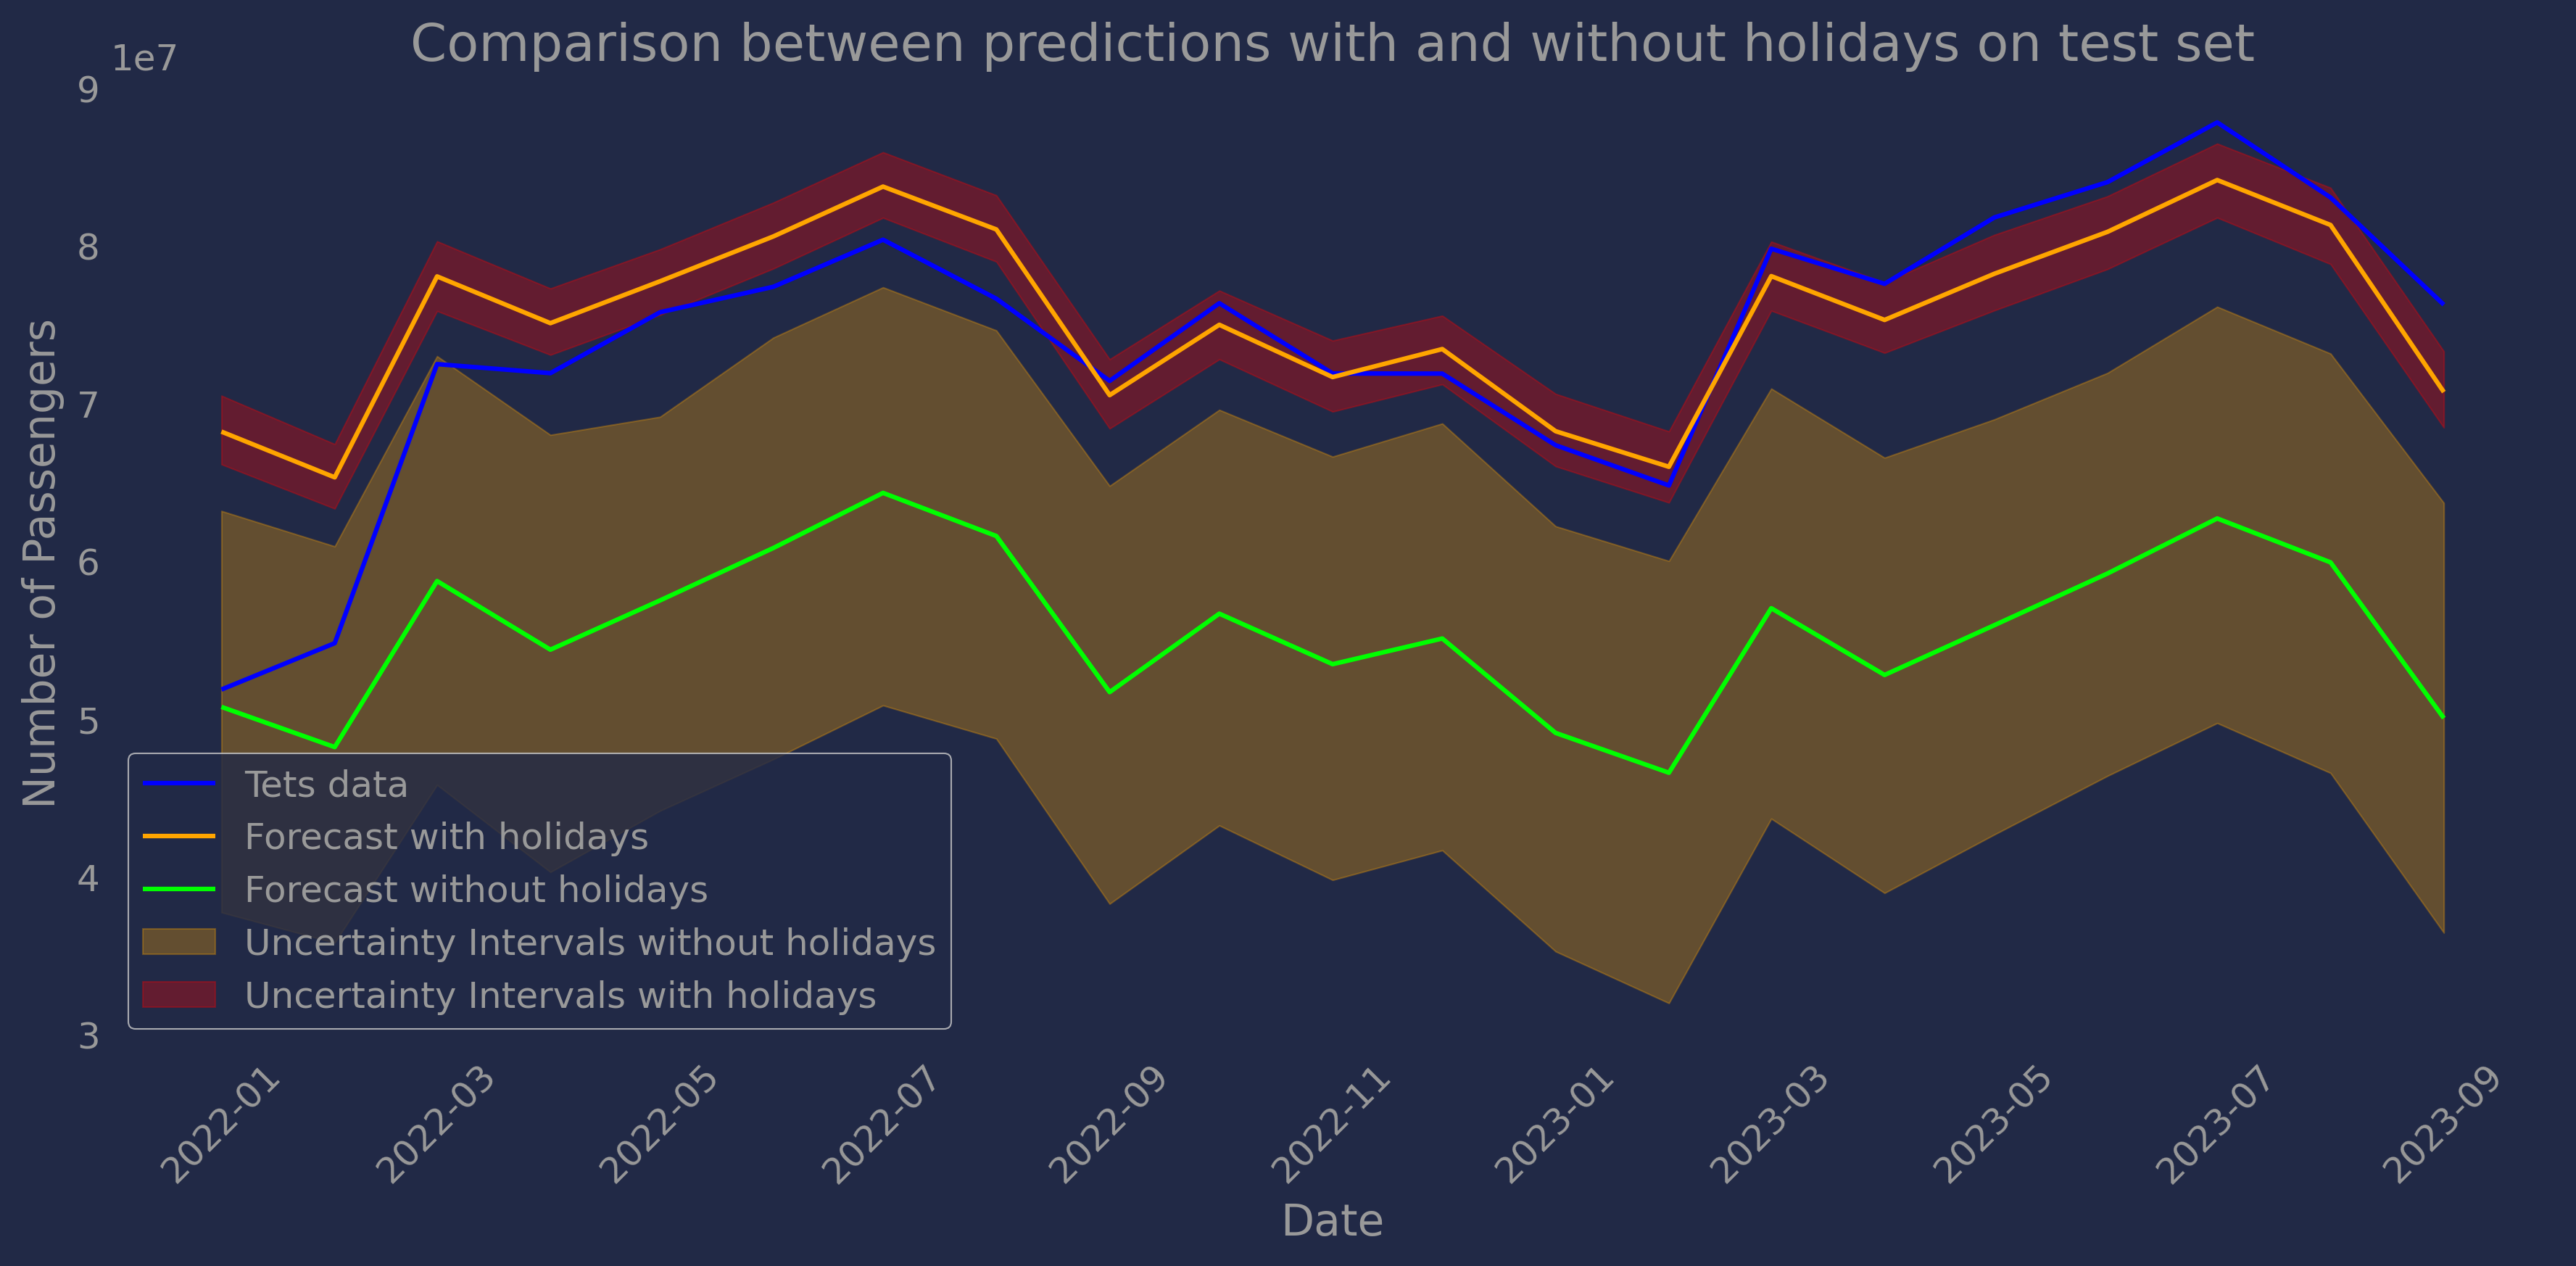
\includegraphics[width=0.8 \textwidth]{comparison.png}
    \caption{Comparación de las predicciones para ambos modelos} 
    \label{fig:fig8}
\end{figure}

Comparando las predicciones del conjunto de prueba para ambos modelos, Figura $~\ref{fig:fig8}$, se aprecia que las predicciones para el segundo modelo son mucho más cercanas a los valores reales que para el primero. Algunos valores reales quedan fuera del intervalo de confianza, pero se quedan mucho más próximos que para el primer modelo. Además, este segundo tiene un error MAPE del $5,47\%$, que es mucho menor que el del modelo anterior. Aquí se puede notar la importacia que ha tenido añadir los festivos al modelo. 

Por último, se propone el modelo con los festivos y con los mejores parámetros, obtenidos de la misma forma que en el apartado ~\ref{sec:8}. Así, se tiene el modelo con los siguientes parámetros: 

\begin{table}[ht] 
\centering
\begin{tabular}{rrr} 
  \hline
 \texttt{changepoint\_prior\_scale} & \texttt{changepoint\_range} & \texttt{seasonality\_prior\_scale} \\ 
  \hline
0.05 & 0.8 & 10.0 \\ 
   \hline
\end{tabular}
\end{table}

\begin{table}[ht] 
\centering
\begin{tabular}{rrrr} 
  \hline
 \texttt{holidays\_prior\_scale} & \texttt{seasonality\_mode} & \texttt{growth} & \texttt{yearly\_seasonality} \\ 
  \hline
10.0 & multiplicative & linear & 20 \\ 
   \hline
\end{tabular}
\caption{Mejores parámetros escogidos} \label{tab:01}
\end{table}

\begin{figure}[h]
    \centering
    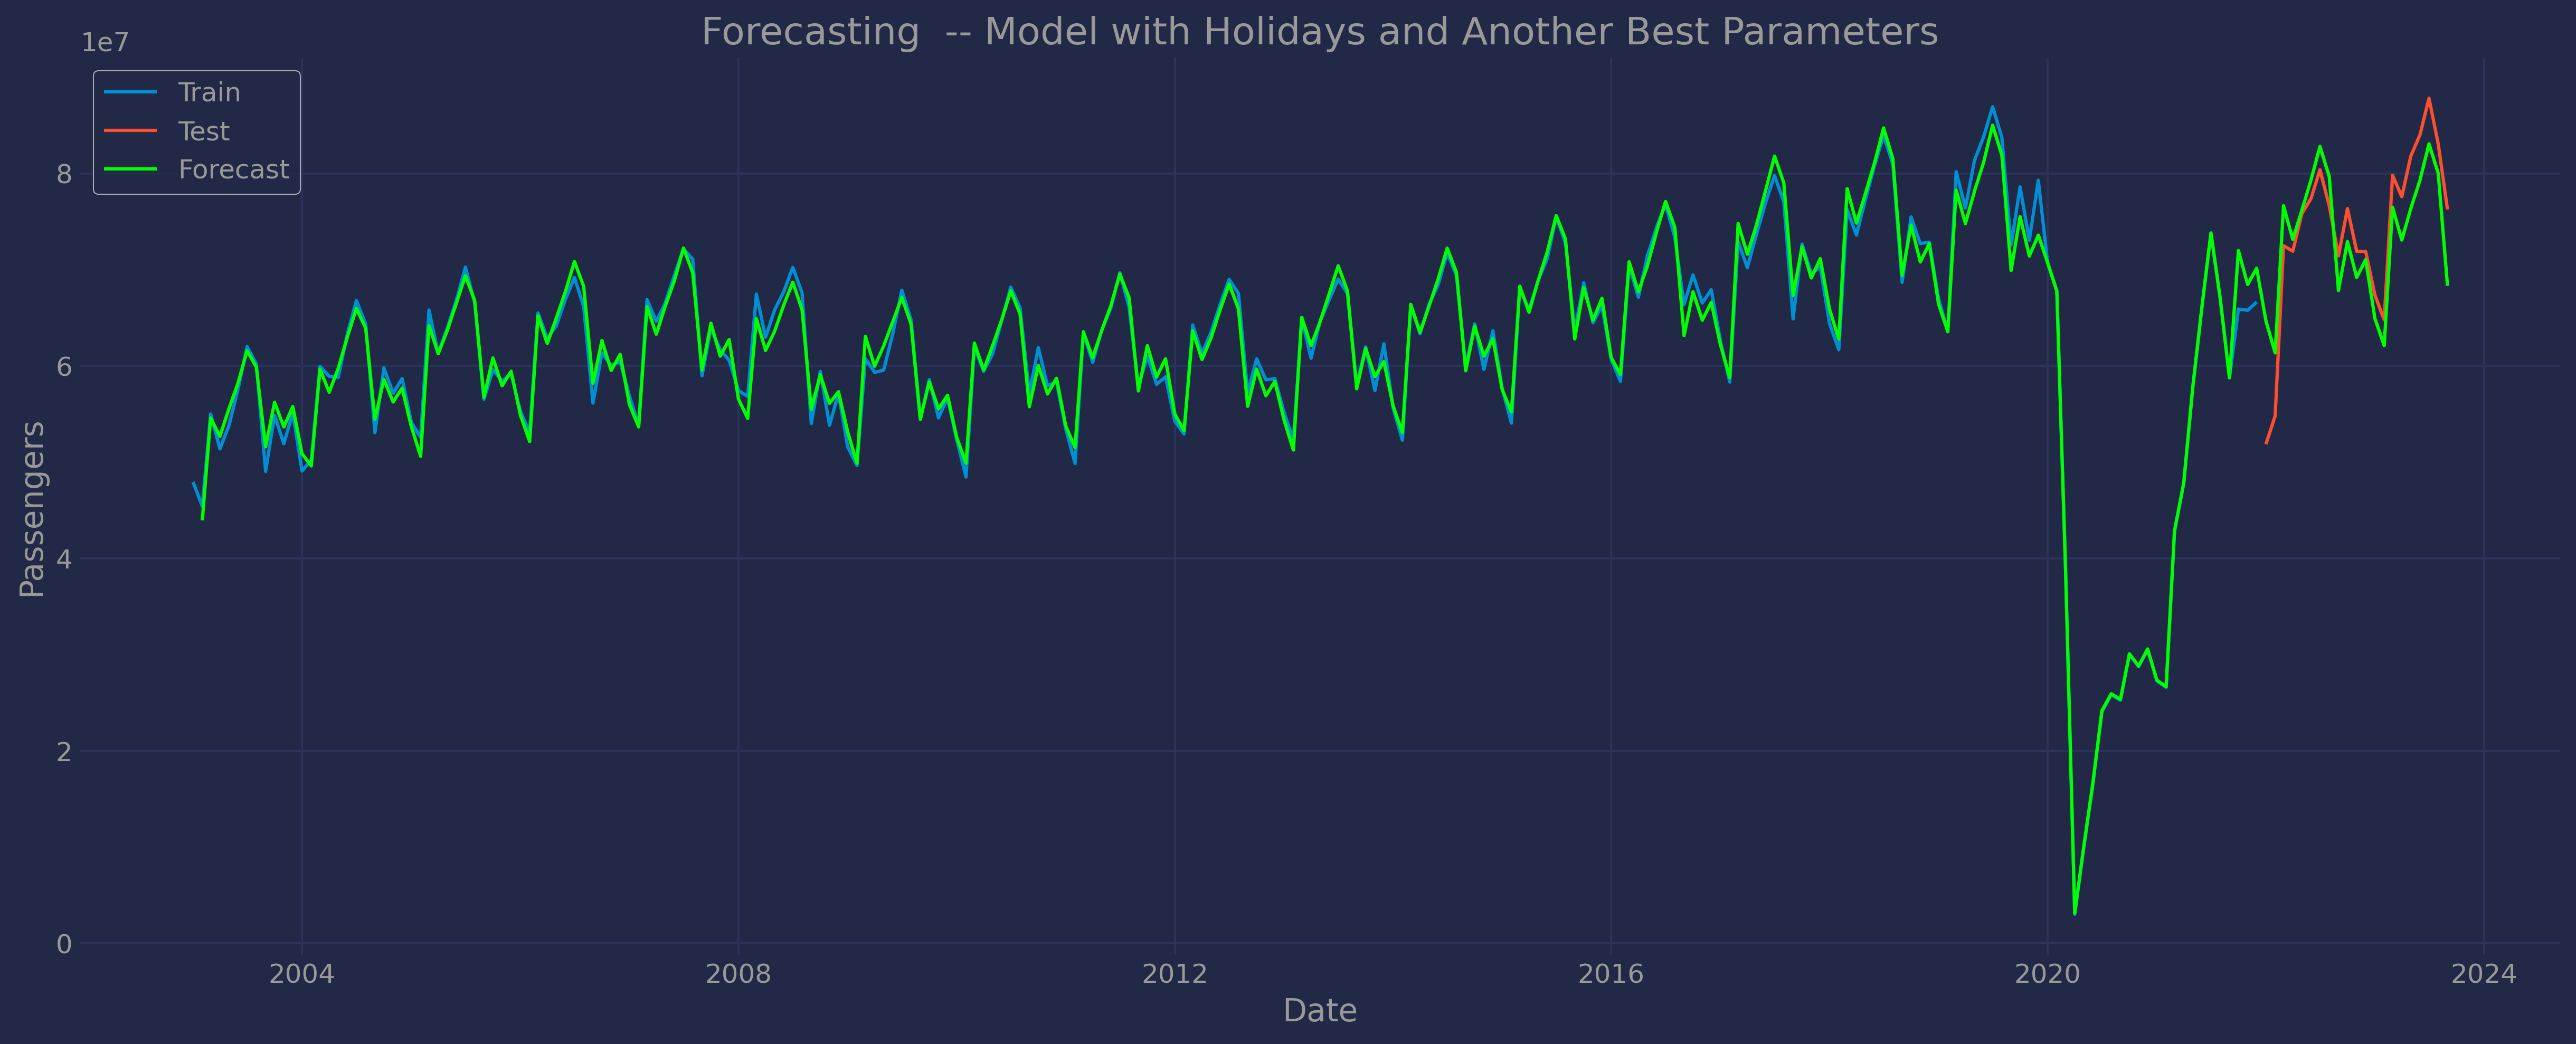
\includegraphics[width=0.8 \textwidth]{fore_best.png}
    %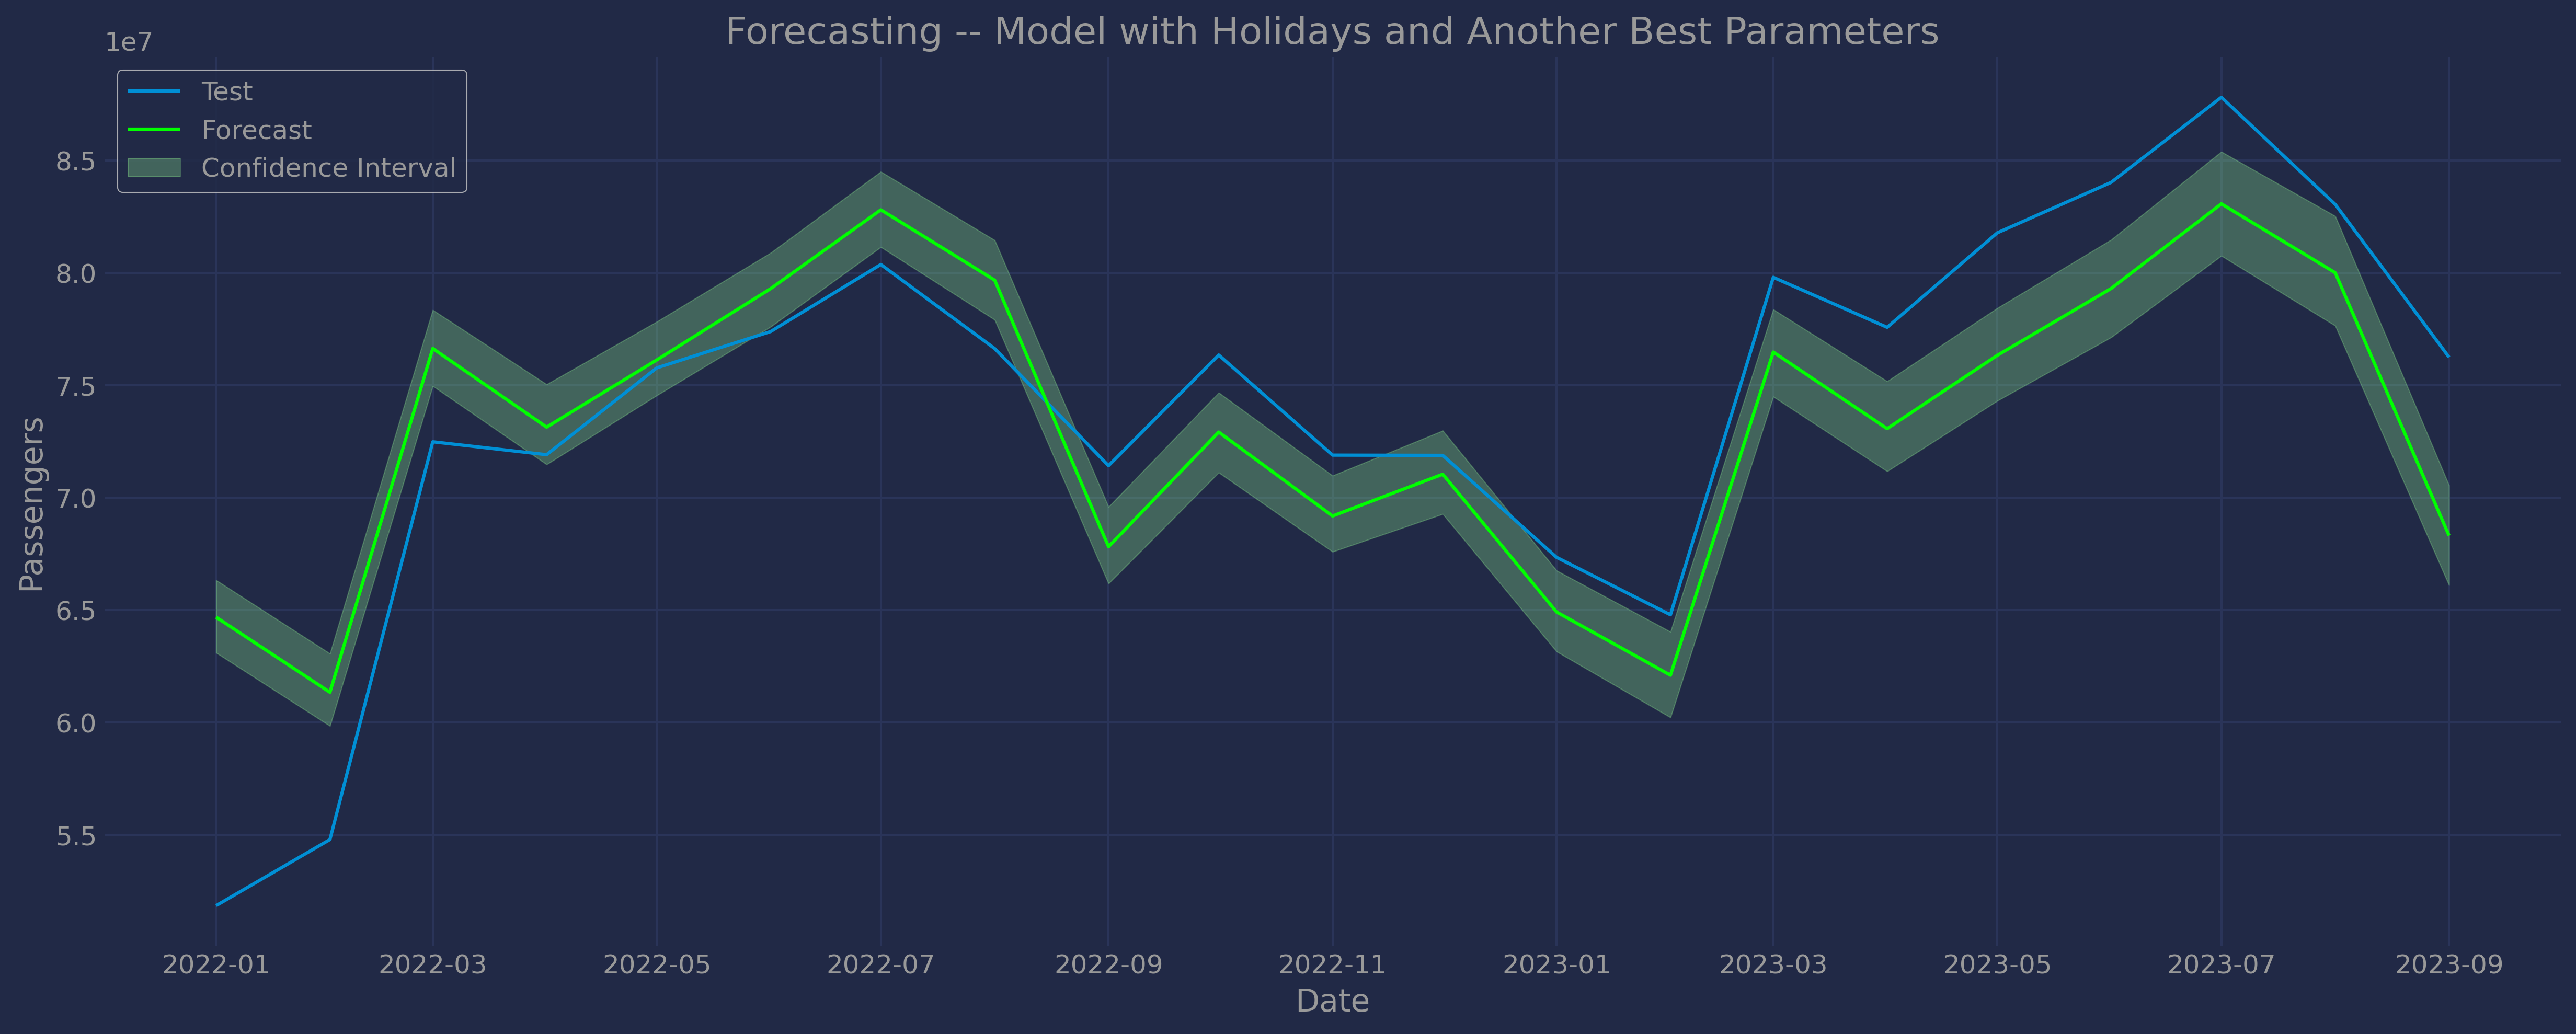
\includegraphics[width=0.8 \textwidth]{pred_best.png}
    %\caption{Predicciones del modelo Prophet con festivos y mejores parámetros para los años 2022-2023} 
    \caption{Predicciones del modelo Prophet con festivos y mejores parámetros}
    \label{fig:fig9}
\end{figure}

En la Figura $~\ref{fig:fig9}$, se puede ver que las predicciones siguen siendo más precisas que para el primer modelo y se adecúa con exactitud a la tendencia y los patrones de los datos. No obstante, este modelo tiene un error MAPE del $5,62\%$, que es ligeramente mayor que el del segundo modelo

\begin{table}[h]
\centering
\begin{tabular}{ccc}
\hline
\textbf{Modelo} & \makecell{\textbf{MAPE del} \\ \textbf{entrenamiento}} & \makecell{\textbf{MAPE del} \\ \textbf{testeo}} \\ \hline
\text{Con valores por defecto} & 25,48\% & 24,41\% \\ \hline
\text{Con valores por defecto + festivos} & 9,83\% & 5,47\% \\ \hline
\text{Con los mejores parámetros + festivos} & 9,75\% & 5,61\% \\ \hline
\end{tabular}
\caption{Errores MAPE del modelo Prophet}
\label{tab:error2.2}
\end{table}

Por consiguiente, comparando los errores MAPE de los tres modelos en la Tabla $~\ref{tab:error2.2}$, se observa que el modelo 2 y 3 es considerablemente mejor al 1, además de caer este primer modelo en \textit{underfitting} por tener errores MAPE demasiado altos para el entrenamiento y el testeo. No obstante, los errores para los modelos 2 y 3 son muy similares, siendo los errores el segundo modelo ligeramente menores a los del tercero, por lo que tratar de elegir los mejores parámetros en este caso no es necesario. Por lo tanto, el mejor modelo es el segundo, el de los valores por defecto más el efecto de los festivos. Por último, se observa que los modelos 2 y 3 no caen en \textit{overfitting} ni \textit{underfitting}, pues aunque los errores en el entrenamiento podrían ser inferiores, se encuentran en un rango razonable.

\begin{figure}[h]
    \centering
    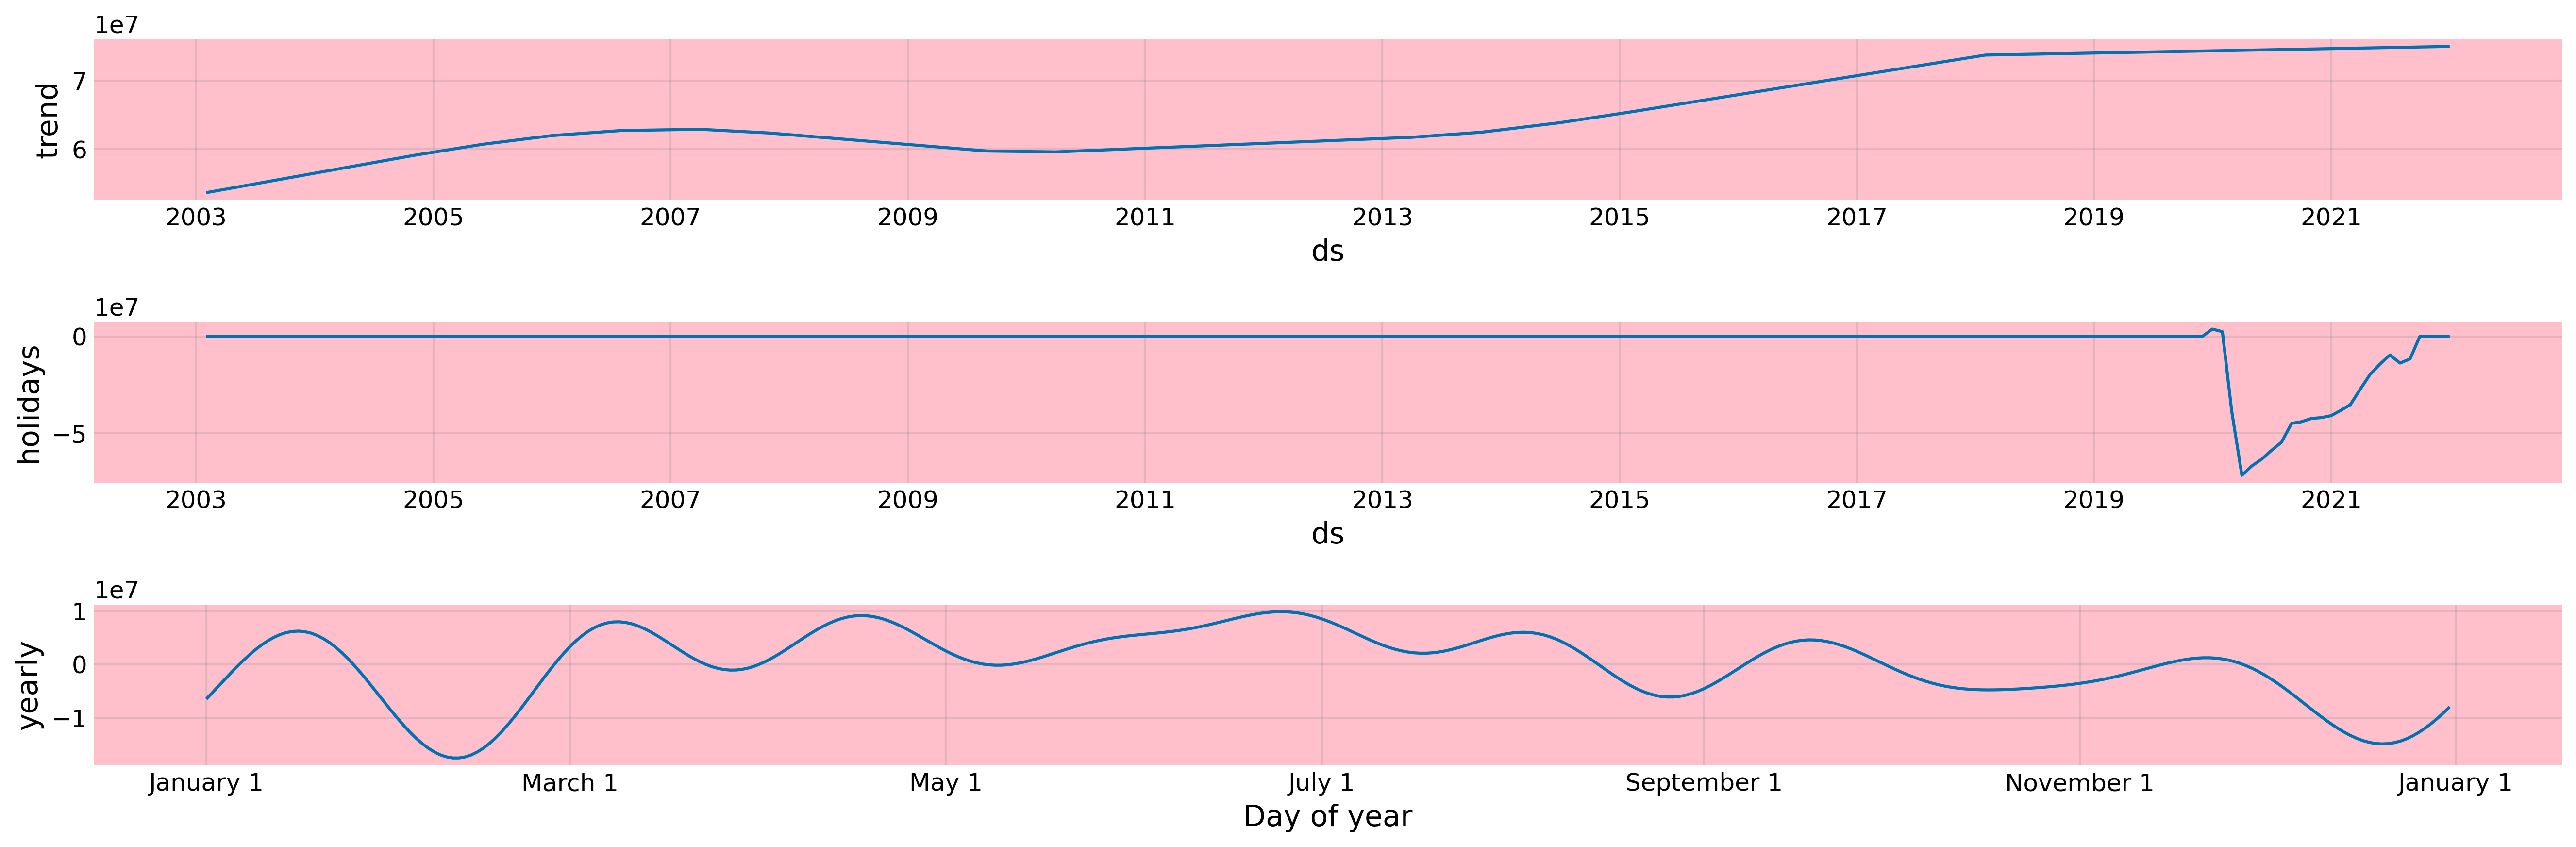
\includegraphics[width=0.8 \textwidth]{componentes_todos.png}
    \caption{Componentes del mejor modelo entrenado }
    \label{fig:fig10}
    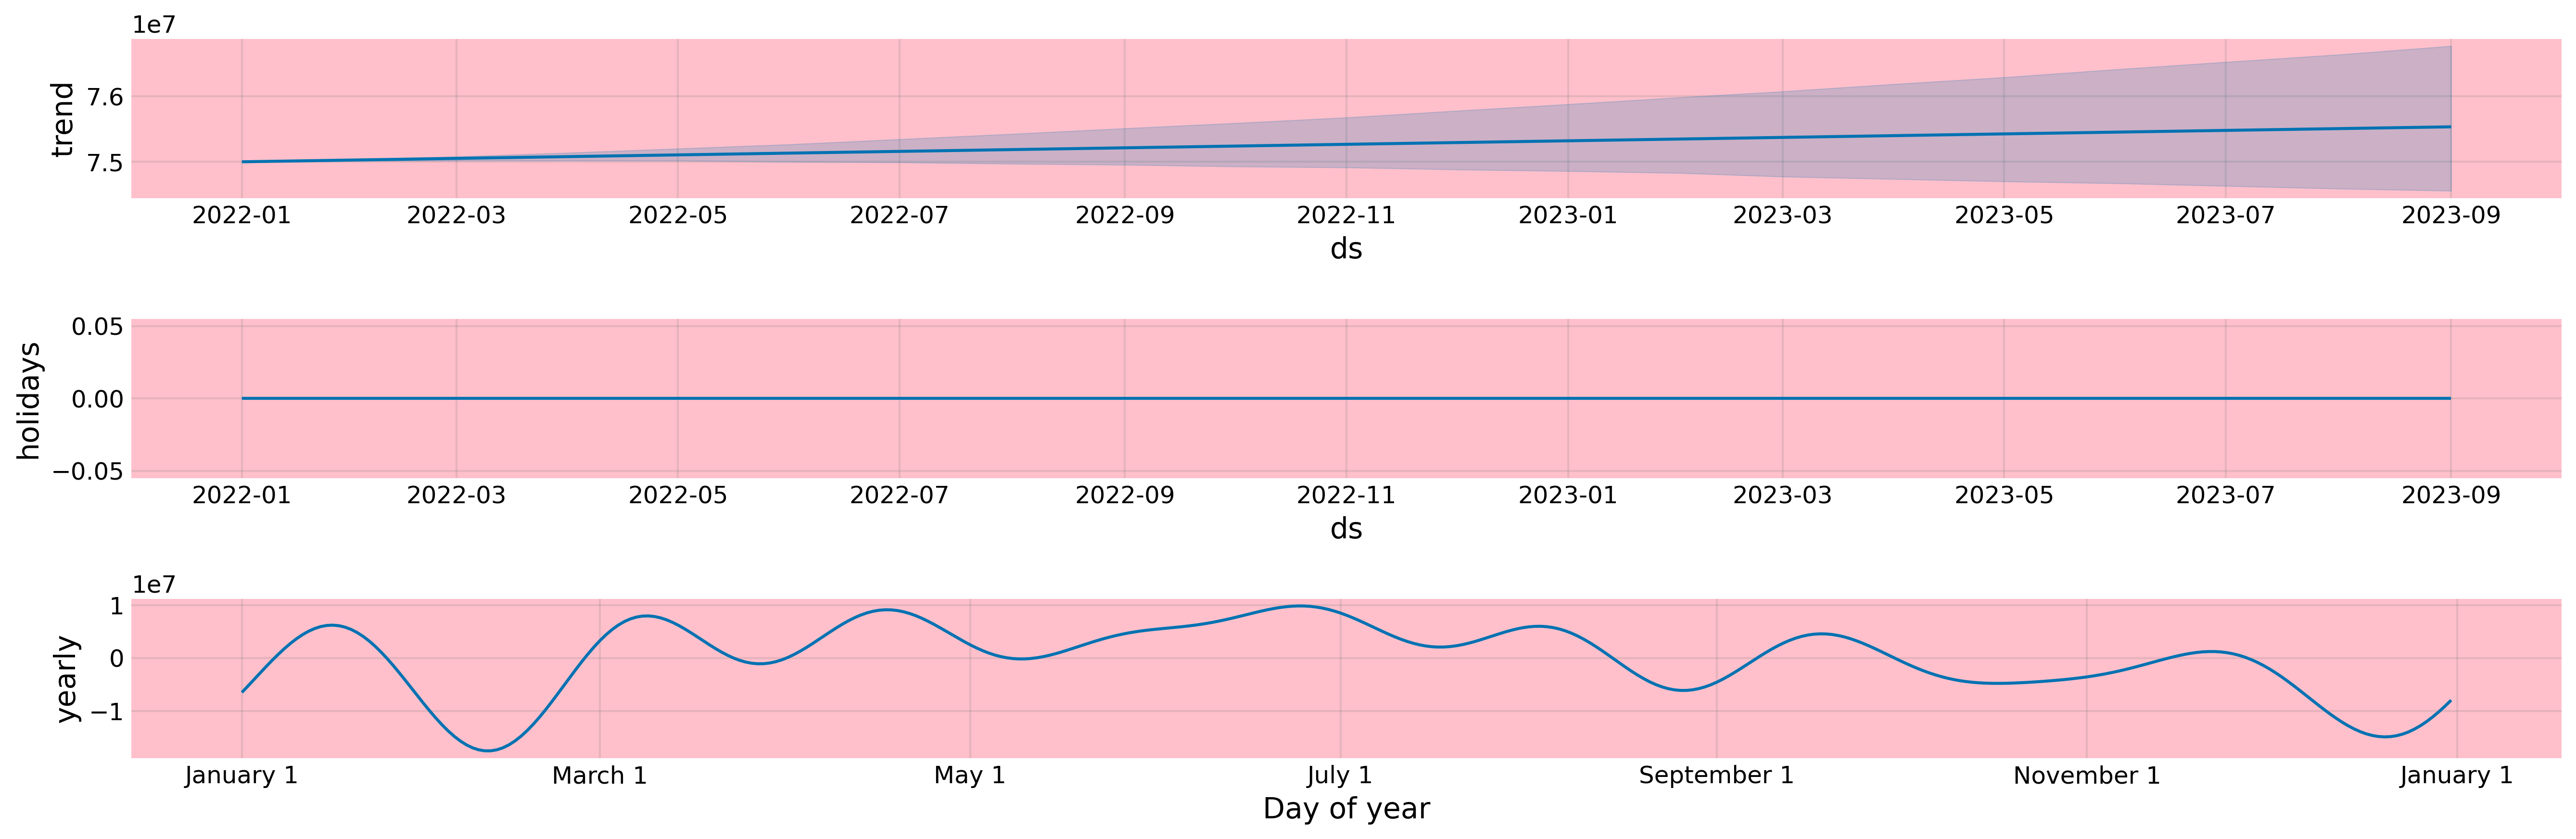
\includegraphics[width=0.8\textwidth]{componentes_test.png}
    \caption{Componentes de la predicción} 
    \label{fig:fig11}
\end{figure}

Finalmente, se pueden ver las componentes del mejor modelo y de su predicción en la Figura $~\ref{fig:fig10}$. Se observa que la tendencia crece progresivamente desde 2003 hasta 2007, entre 2007 y 2008 hasta 2010 decrece ligeramente (posiblemente a causa de crisis financiera de 2008) y luego vuelve a crecer cada vez de forma mas pronunciada hasta 2019, donde se mantiene estable hasta 2021 debido al COVID. En cuanto a la componente anual, se aprecian picos y valles, que sugieren que en ciertas épocas del año hay aumentos y disminuciones en el número de personas que toman un avión.

Por su parte, para la predicción (Figura $~\ref{fig:fig11}$), se observa que la tendencia sigue un crecimiento lineal, sin cambios en la pendiente. También, en la componente estacional anual se aprecian los mismos cambios que para el modelo, por lo que las predicciones del modelo siguen bien los patrones de los datos. Para el efecto de fectivos, la línea es bastante plana, lo que indica que estos festivos no han tenido gran impacto en la predicción.










\newpage


\section{Redes Neuronales}\label{sec:10}

Una red neuronal \cite{redes1} es un modelo computacional o de aprendizaje automático que se basa en el funcionamiento del cerebro humano, utilizando procesos que imitan la forma en que las neuronas biológicas trabajan juntas para identificar fenómenos, hacer inferencias y llegar a conclusiones.

\begin{figure}[h]
    \centering
    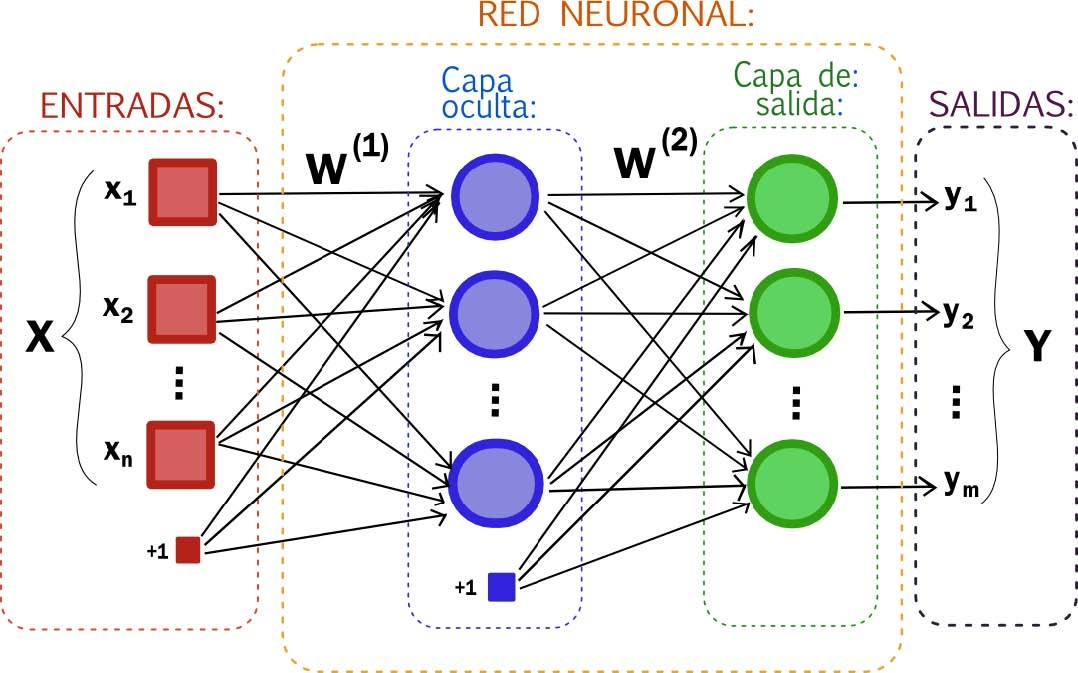
\includegraphics[width=0.55 \textwidth]{foto1.jpeg}
    \caption{Red neuronal con una capa oculta, $n$ neuronas de entradas y $m$ neuronas de salida.} 
    \label{fig:fig12}
\end{figure}

La estructura de una red neuronal \cite{redes4} se basa en capas interconectadas, y cada capa contiene neuronas. Una neurona es una unidad que transforma una combinación lineal de entradas mediante una función no lineal. La primera capa se denomina capa de entrada (donde se introducen los datos) y la última, capa de salida, a partir de la cual se generan las salidas o predicciones. Las capas intermedias se denominan capas ocultas. Si la red neuronal tiene solo una capa oculta, se conoce como red neuronal poco profunda (\textit{shallow neural network}); mientras que si tiene más de una capa oculta, se conoce como red neuronal profunda (\textit{deep neural network}).

La unidad básica de red neuronal es el perceptrón, que fue la primera red neuronal que se diseñó (en 1957 por Frank Rosenblatt). Esta tiene una sola capa oculta con una única neurona y en su capa de salida se encuentra únicamente una neurona.

Para poner en funcionamiento la red neuronal, se necesitan tres elementos: 

\begin{enumerate}
    \item \textbf{Pesos ($W$)}: son los parámetros que ponderan las entradas de la red. Cada conexión entre neuronas tiene un peso asociado que determina la importancia de esa conexión en el proceso de aprendizaje.
    \item \textbf{Bias ($b$)}: también conocido como término independiente o sesgo, es un valor adicional que se suma al resultado de la multiplicación de los pesos por las entradas. El bias permite que la red aprenda mejor desplazando la función de activación y ayudando a que el modelo sea más flexible.
    \item \textbf{Funciones de activación}: son funciones que determinan si una neurona debe activarse o no; es decir, si debe transmitir su señal a la siguiente capa. Sin las funciones de activación, las redes neuronales no podrían resolver problemas complejos.
\end{enumerate}

Las funciones de activación \cite{redes5} son funciones no lineales esenciales para las redes neuronales porque aportan la no-linealidad al modelo, lo que hace que el modelo sea más complejo y aprenda de relaciones no lineales. Si no se introdujeran funciones de activación, entonces en cada neurona simplemente se aplicaría una regresión lineal, por lo que toda la red neuronal equivaldría a una regresión lineal. Se necesitan que estas funciones sean diferenciables y monótonas. Las principales funciones de activación son:

\begin{itemize}
    \item Función de activación lineal: $lineal(x) = x$
    \item Función sigmoide: $sig(x) = \frac{1}{1 + e^{-x}}$
    \item Función tangente hiperbólica: $\tanh(x) = \frac{e^{x} - e^{-x}}{e^{x} + e^{-x}}$
    \item Función ReLU (\textit{Rectified Linear Unit}): $\text{ReLU}(z) =
    \begin{cases} 
    z & \text{si } z > 0 \\
    0 & \text{si } z \leq 0
    \end{cases}$
    \item Función Leaky ReLU: $\text{Leaky ReLU}(x) = \begin{cases} 
    x & \text{si } x > 0 \\
    \alpha x & \text{si } x \leq 0 
    \end{cases}$
    \item Función Softmax: $\text{Softmax}(x_i) = \frac{e^{x_i}}{\sum_{j=1}^{n} e^{x_j}}$
\end{itemize}

Las sigmoide y la tangente hiperbólica se suele utilizar para problemas de clasificación binaria y softmax para clasificación multiclase, mientras que la función ReLU y Leaky ReLU se usan tanto para problemas de clasificación como para de regresión.

Por otro lado, la sigmoide y Softmax se usan en las capas de salidad; mientras que la tangente hiperbólica, ReLU y Leaky ReLU se usan en las capas ocultas.

\subsection{Aprendizaje de una red neuronal}\label{sec:11}
\subsubsection{Propagación hacia delante}\label{sec:12}

El primer paso para inicializar una red neuronal es la propagación hacia delante \cite{redes2}, que consiste en hacer pasar los datos de entrada a través de las distintas capas de la red. En cada neurona, los valores de entrada son transformados mediante una combinación lineal de pesos y sesgos, seguidos por la aplicación de una función de activación no lineal. Se podría decir que cada neurona es equivalente a una regresión lineal seguida de una transforación no lineal. Este proceso continúa hasta la capa de salida, donde se obtiene el resultado final de la red.

Consideremos una red neuronal con L capas, $L \in \mathbb{N}$, y que cada capa tiene $l_r$ neuronas, $r \in \{1, ..., L\}$. Sean:

\begin{itemize}
    \item $X = [x_1, \dots, x_{T}]^T$ la matriz de los datos de entrada, con $T$ el número de neuronas de la capa de entrada.
    \item $w_{ij}^{(h)}$ el peso de la neurona j-ésima de la capa $(h-1)$ hacia la neurona i-ésima de la capa $h$.
    \item $W^{(i)} = [w_{pq}^{(i)}]$ con $1 \leq p \leq l_{i-1},1 \leq q \leq l_{i}$ la matriz de pesos de la capa (i-1)-iésima a la capa i-ésima.
    \item $z^{(i)} = [z_1^{(i)}, \dots, z_{l_i}^{(i)}]^T$ las preactivaciones de la capa i-ésima.
    \item $f^{(i)}$ es la función de activación de la capa i-ésima.
    \item $a^{(i)} = [a_1^{(i)}, \dots, a_{l_i}^{(i)}]^T$ la activación de la capa i-ésima, con $a^{(0)} = X$
    \item $b^{(i)} = [b_1^{(i)}, \dots, b_{l_i}^{(i)}]^T$ el bias de la capa i-ésima.
\end{itemize}

La propagación hacia adelante se lleva a cabo aplicando, de manera iterativa para cada capa i-ésima, las siguientes ecuaciones:

\begin{equation}
z^{(i)} =
\begin{bmatrix}
z_1^{(i)} \\
\vdots \\
z_{l_i}^{(i)}
\end{bmatrix}
=
W^{(i)} a^{(i-1)} + b^{(i)}
\quad \text{;} \quad
a^{(i)} = 
\begin{bmatrix}
a_1^{(i)} \\
\vdots \\
a_{l_i}^{(i)}
\end{bmatrix}
=
f^{(i)}(z^{(i)})
=
\begin{bmatrix}
f^{(i)}(z_1^{(i)}) \\
\vdots \\
f^{(i)}(z_{l_i}^{(i)})
\end{bmatrix}
\end{equation}

Finalmente, la salida de la red es:

\begin{equation}
\hat{Y}=a^{(L)}= f^{(L)}(z^{(L)}) = f^{(L)}(W^{(L)}a^{(L-1)} + b^{(L)})
\end{equation}

\subsubsection{\textit{Backpropagation} o propagación hacia atrás}\label{sec:13}

Después de la propagación hacia delante, el siguiente paso en el entrenamiento de una red neuronal es la propagación hacia atrás (\textit{backpropagation}), que se encarga de ajustar los pesos y los sesgos para minimizar el error de la red.

En primer lugar, vamos a definir dos productos matriciales:

\begin{definition} Dadas dos matrices $A$ y $B$ de dimensiones $m \times n$, su producto de Hadamard $C = A \circ B$ se define como:

\begin{equation}
c_{ij} = a_{ij} \cdot b_{ij}
\end{equation}

donde \(c_{ij}\) representa el elemento de la fila \(i\) y columna \(j\) de la matriz resultante.
\end{definition}

\begin{definition}
Dadas dos matrices A de dimensión $n \times 1$ y B de dimensión $m \times 1$, su producto externo, denotado por $outer$, se define como $outer(A,B) = AB^T$.
\end{definition}

Para llevar a cabo la propagación hacia atrás, empleamos el algoritmo del descenso del gradiente y utilizamos como función de coste a minimizar la función del error MSE, que es la más común para series temporales para ajustar los parámetros.

\begin{equation}
J(W, b) = \frac{1}{T} \sum_{i=1}^{T} (y_i - \hat{y}_i)^2
\end{equation}

Esta función depende de $W$ y $b$ porque son los parámetros que queremos actualizar. Para cada capa $i \in \{1, ..., L\}$, definimos un error $e^{(i)}$ y un gradiente de error $\delta^{(i)}$. Para la capa de salida $L$, se tiene:

\begin{equation}
e^{(L)} = Y - a^{(L)}
\quad \text{;} \quad
\delta^{(L)} = f'^{(L)}(z^{(L)}) \circ e^{(L)}
\end{equation}

Para cada capa oculta $l \in \{1,2, ..., L-2, L-1\}$, tenemos:

\begin{equation}
e^{(l)} = W^{(l+1)^T} \delta^{(l+1)}
\quad \text{;} \quad
\delta^{(l)} = f'^{(l)}(z^{(l)}) \circ e^{(l)}
\end{equation}

Para llevar a cabo el descenso del gradiente, necesitamos calcular las derivadas parciales de la función de coste $J$ con respecto a estos parámetros. Aplicando la regla de la cadena, se obtiene: 

\begin{equation}
\frac{\partial J}{\partial W^{(i)}} = \frac{2}{N}\left(outer(\delta^{(i)}, a^{(i-1)})\right)
\quad \text{;} \quad
\frac{\partial J}{\partial b^{(i)}} = \frac{2}{N} \delta^{(i)}
\end{equation}

Entonces, los nuevos pesos y sesgos serán de la forma:

\begin{equation}
W^{(l)} - \eta\frac{\partial J}{\partial W^{(l)}}
\quad \text{;} \quad
b^{(l)} - \eta \frac{\partial J}{\partial b^{(l)}}
\end{equation}


Así pues, los pesos y los sesgos actualizados quedan como:
\begin{equation}
W^{(i)} \leftarrow W^{(i)} - \eta \frac{2}{T}\left(outer(\delta^{(i)}, a^{(i-1)})\right)
\quad \text{;} \quad
b^{(i)} \leftarrow b^{(i)} - \eta\frac{2}{T} \delta^{(i)}, 
\end{equation}

donde $\eta$ es la tasa de aprendizaje (por ejemplo, si tenemos una tasa de aprendizaje de $0.01$, significa que en cada paso del descenso de gradiente, los pesos y sesgos se ajustarán un $1 \%$ de la dirección del gradiente) y T es el número de datos de los que se dispone.

Por último, cuando la red va hacia delante y hacia atrás una vez, se dice que ha realizado una época de entrenamiento (\textit{epoch}). Para parar el entrenamiento de una red neuronal, lo más común es darle un número finito de \textit{epoches} que puede realizar o darle una cota para el error; es decir, cuando el error que se comete es menor que el impuesto, se detiene el entrenamiento.



\subsection{Redes Neuronales Recurrentes}\label{sec:14}

 Las Redes Neuronales Recurrentes (\textit{Recurrent Neural Networks} o RNN) \cite{rnn1} son un tipo de redes neuronales diseñadas para procesar datos que siguen un orden secuencial. Hasta ahora, la información fluía en una sola dirección: desde la entrada hasta la salida pasando por las capas ocultas. Ahora, las RNN tienen memoria, lo que les permite recordar información pasada y utilizarla para predecir datos futuros en la secuencia. Hay diversos tipos de RNN, pero en esta sección nos centraremos en las RNN simples (también conocidas como RNN \textit{vanilla} o vainilla).


\begin{figure}[h]
    \centering
    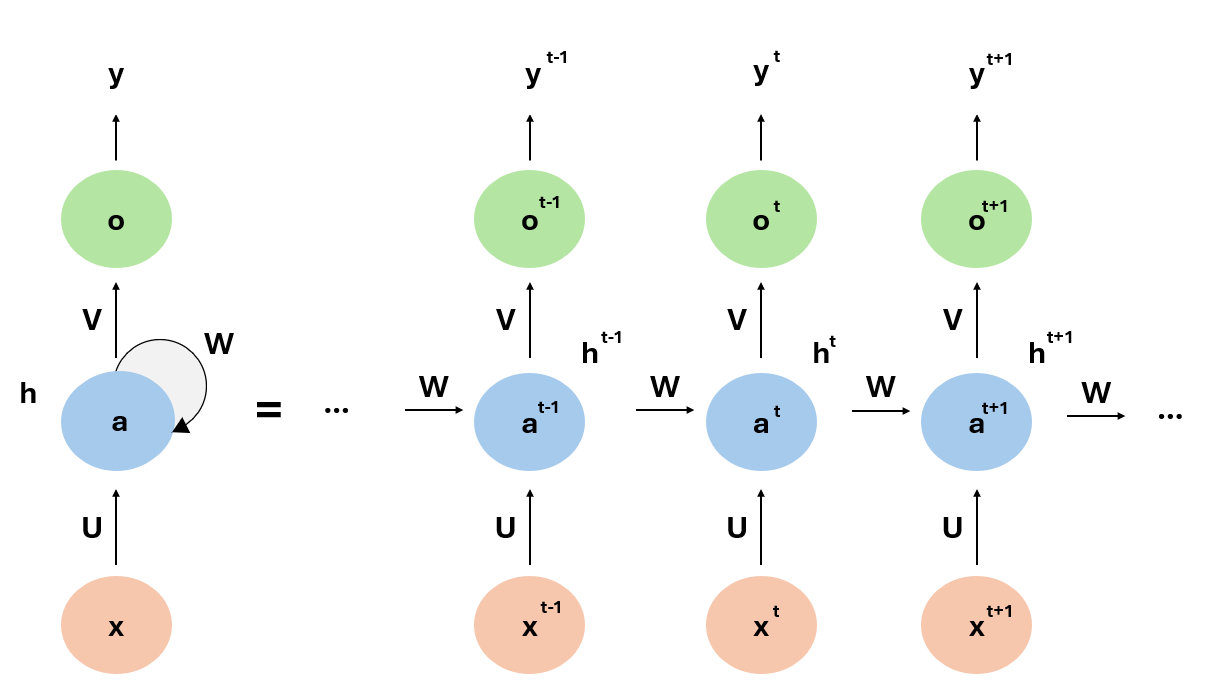
\includegraphics[width=0.55 \textwidth]{foto2.png}
    \caption{Estructura de una red RNN desplegada en el tiempo} 
    \label{fig:fig13}
\end{figure}

En general, las arquitectura de las RNN mantienen similitudes con las redes neuronales tradicionales, pero introduce conexiones recurrentes que permiten el flujo de información a través del tiempo. Ahora, empezamos con una capa de entrada donde se sitúan los datos conocidos, continuamos con un estado oculto donde se producen las conexiones temporales y acabamos con la capa de salida, En la Figura $~\ref{fig:fig13}$ se pueden ver el despliegue de una RNN en el tiempo. 

A continuación, se desarrollará el aprendizaje \cite{rnn2} de una RNN:

\subsubsection{Propagación hacia delante}\label{sec:15}


Considérese una serie temporal $\{X_t\}$ con T elementos y sean $n,m,p \in \mathbb{N}$. Antes de inicializar la RRN, se denotan algunos elementos: 

\begin{itemize}
    \item $x^{(t)} \in \mathbb{R}^n$ el dato de entrada en ese instante t.
    \item $h^{(t)} \in \mathbb{R}^m$ el estado oculto en el instante t. Representa la memoria de la red hasta ese momento.
    \item $U \in \mathbb{M}_{m \times n}(\mathbb{R})$ los pesos de entrada a los estados.
    \item $V \in \mathbb{M}_{p \times m}(\mathbb{R})$ los pesos de estado a la salida.
    \item $W \in \mathbb{M}_{m \times m}(\mathbb{R})$ los pesos de estado a estado.
    \item $b_h \in \mathbb{R}^m$ los sesgos del estado oculto.
    \item $b_y \in \mathbb{R}^p$ los sesgos de la salida.
    \item $f,g$ dos funciones de activación. Usualmente, se toma $f$ como $ReLU$ o $tanh$ para introducir la no linealidad en el estado oculto, y se toma $g$ como la identidad o $softmax$.
\end{itemize}

Ahora bien, la propagación hacia delante comienza con la especificación de un estado inicial $h^{(0)}$ (comúnmente, se toma el vector nulo). Entonces, para cada etapa desde $t=1$ hasta $t=T$, aplicamos las siguientes ecuaciones: 

\begin{equation}
\begin{aligned}
a^{(t)} &= b_h + W h^{(t-1)} + U x^{(t)} \\
h^{(t)} &= f(a^{(t)}) \\
o^{(t)} &= b_y + V h^{(t)} \\
\hat{y}^{(t)} &= g(o^{(t)})
\end{aligned}
\end{equation}


Y, de esta forma, obtendríamos $x_{T+1}=\hat{y}^{(T)}$.


\subsubsection{\textit{Back Propagation Through Time} o BPTT}\label{sec:16}

Ahora, para poder entrenar la RNN adecuadamente, se necesita poder volver hacia atrás. Esto se lleva a cabo con el método BPTT como propagación hacia atrás \cite{rnn3}, que se basa en el método \textit{backpropagation} de las redes neuronales tradicionales, pero con ciertas modificaciones. Ahora, se quieren actualizar las tres matrices de pesos $U$,$V$ y $W$ y los dos vectores de sesgos $b_h$ y $b_y$. Antes de comenzar, se define un nuevo producto: 

\begin{definition} Sea $A$ una matriz de dimensión $m \times n$ y B una matriz de dimensión $p \times q$, se define su producto de Kronecker $C = A \otimes B$ se define como:

\begin{equation}
C = 
\begin{bmatrix}
a_{11} B & a_{12} B & \cdots & a_{1n} B \\
a_{21} B & a_{22} B & \cdots & a_{2n} B \\
\vdots   & \vdots   & \ddots & \vdots \\
a_{m1} B & a_{m2} B & \cdots & a_{mn} B
\end{bmatrix}
\end{equation}

donde C es una matriz de dimensión $mp \times nq$.
\end{definition}

Así pues, sea $L$ la función de coste a minimizar (no se especifica cuál es, pero se puede considerar, por ejemplo, la función del error MSE para tareas de regresión o la función de la entropía cruzada para problemas de clasificación). Entonces, se puede escribir $L = \sum_{t=1}^{T} l^{(t)}$, con $l^{(t)}$ dependiendo del valor real $y^{(t)}$ y del valor predicho $\hat{y}^{(t)}$ para cada instante de tiempo $t$, pues en cada instante de tiempo se produce un costo.

Considérese un instante de tiempo $t \in \{1,...,T\}$, aplicando la regla de la cadena se tiene: 

\begin{equation}
\frac{\partial L}{\partial o^{(t)}} = \frac{\partial L}{\partial l^{(t)}} \frac{\partial l^{(t)}}{\partial \hat{y}^{(t)}} \frac{\hat{y}^{(t)}}{\partial o^{(t)}} = \frac{\partial l^{(t)}}{\partial \hat{y}^{(t)}} g'(o^{(t)}) \in \mathbb{R}^p
\end{equation}

\begin{equation}
\frac{\partial L}{\partial h^{(t)}} = \left( \frac{\partial o^{(t)}}{\partial h^{(t)}} \right )^T \frac{\partial L}{\partial o^{(t)}} + \frac{\partial L}{\partial h^{(t+1)}}\frac{\partial h^{(t+1)}}{\partial h^{(t)}}
\end{equation}

Se denota $\delta^{(t)} = \frac{\partial L}{\partial h^{(t)}}$. Se observa que:

\begin{equation}
\frac{\partial h^{(t+1)}}{\partial h^{(t)}} = \left( \frac{\partial a^{(t)}}{\partial h^{(t)}} \right)^T \frac{\partial h^{(t+1)}}{\partial a^{(t)}} = W^T f'(a^{(t)})I_{m \times m} \in \mathbb{R}^m
\end{equation}

Así, se obtiene que:

\begin{equation}
\frac{\partial L}{\partial h^{(t)}} = \delta^{(t)} = V^T \frac{\partial l^{(t)}}{\partial \hat{y}^{(t)}} g'(o^{(t)}) + \delta^{(t+1)} W^T f'(a^{(t)})I_{m \times m} \in \mathbb{R}^m
\end{equation}

Nótese que si $t=T$, entonces $\delta^{(T)} = V^T \frac{\partial l^{(T)}}{\partial \hat{y}^{(T)}} g'(o^{(T)})$.

\begin{equation}
\left( \frac{\partial h^{(t)}}{\partial W} \right)^T = \left( \frac{\partial h^{(t)}}{\partial a^{(t)}} \frac{\partial a^{(t)}}{\partial W} \right)^T = (h^{(t-1)} \otimes I_{m \times m}) f'(a^{(t)}) I_{m \times m}
\end{equation}

Ahora, 
\begin{equation}
(h^{(t-1)} \otimes I_{m \times m}) f'(a^{(t)}) I_{m \times m}\delta^{(t)} = vec(f'(a^{(t)}) I_{m \times m}\delta^{(t)}h^{(t-1)^T})
\end{equation}

Análogamente, se tiene que
\begin{equation}
\left( \frac{\partial h^{(t)}}{\partial U} \right)^T = (x^{(t)} \otimes I_{m \times m}) f'(a^{(t)}) I_{m \times m}
\end{equation}
\begin{equation}
(x^{(t)} \otimes I_{m \times m}) f'(a^{(t)}) I_{m \times m}\delta^{(t)} = vec(f'(a^{(t)}) I_{m \times m}\delta^{(t)}x^{(t)^T})
\end{equation}




Por tanto, se está en condiciones de calcular los parámetros a actualizar: 

\begin{enumerate}
    \item \[\frac{\partial L}{\partial U} = \sum_{t=1}^{T} vec_{p \times p}^{-1} \left( \left( \frac{\partial h^{(t)}}{\partial U} \right)^T \frac{\partial L}{\partial h^{(t)}} \right) = \sum_{t=1}^{T} vec_{p \times p}^{-1} \left( (x^{(t)} \otimes I_{m \times m}) f'(a^{(t)}) I_{m \times m} \delta^{(t)} \right) =
    \]
    \begin{equation}
    = \sum_{t=1}^{T}f'(a^{(t)}) I_{m \times m}\delta^{(t)}(x^{(t))^T} \in \mathbb{M}_{m \times n}(\mathbb{R})
    \end{equation}
    \item \begin{equation} \frac{\partial L}{\partial V} = \sum_{t=1}^{T} \frac{\partial L}{\partial o^{(t)}} \frac{\partial o^{(t)}}{\partial V} = \sum_{t=1}^{T} \frac{\partial l^{(t)}}{\partial \hat{y}^{(t)}} g'(o^{(t)})(h^{(t)})^T \in \mathbb{M}_{p \times m}(\mathbb{R})
    \end{equation}
    \item \[ \frac{\partial L}{\partial W} = \sum_{t=1}^{T} vec_{p \times p}^{-1} \left( \left( \frac{\partial h^{(t)}}{\partial W} \right)^T \frac{\partial L}{\partial h^{(t)}} \right) = \sum_{t=1}^{T} vec_{p \times p}^{-1} \left( (h^{(t-1)} \otimes I_{m \times m}) f'(a^{(t)}) I_{m \times m} \delta^{(t)} \right) =
    \]
    \begin{equation}
    = \sum_{t=1}^{T}f'(a^{(t)}) I_{m \times m}\delta^{(t)}(h^{(t-1)})^T \in \mathbb{M}_{m \times m}(\mathbb{R})
    \end{equation}
    \item \begin{equation} \frac{\partial L}{\partial b_h} = \sum_{t=1}^{T} \left( \frac{\partial h^{(t)}}{\partial b_h}\right)^T \frac{\partial L}{\partial h^{(t)}} = \sum_{t=1}^{T} \left( \frac{\partial h^{(t)}}{\partial a^{(t)}} \frac{\partial a^{(t)}}{\partial b_h}\right)^T \frac{\partial L}{\partial h^{(t)}} =
    \sum_{t=1}^{T} f'(a^{(t)}) I_{m \times m} \delta^{(t)} \in \mathbb{R}^m
    \end{equation}
    \item \begin{equation} \frac{\partial L}{\partial b_y} = \sum_{t=1}^{T} \frac{\partial L}{\partial l^{(t)}} \frac{\partial l^{(t)}}{\partial \hat{y}^{(t)}} \frac{\partial \hat{y}^{(t)}}{\partial o^{(t)}} \frac{\partial o^{(t)}}{\partial b_y} = \sum_{t=1}^{T} \frac{\partial l^{(t)}}{\partial \hat{y}^{(t)}} g'(o^{(t)}) \in \mathbb{R}^p
    \end{equation}

\end{enumerate}

Por consiguiente, las matrices de pesos y los vectores de sesgos se actualizan de la siguiente manera: 

\begin{equation}
\theta \leftarrow \theta - \eta  \frac{\partial L}{\partial \theta}, \forall \theta \in \{U,V,W,b_h,b_y, h_t \} \text{  }\text{ y }\text{  } \forall t \in \{ 1,...,T\},
\end{equation}

donde $\eta$ es la tasa de aprendizaje.

Sin embargo, las RNN puede generar problemas si el número de \textit{epoches} es demasiado elevado. Las matrices de pesos con las que se obtienen los estados ocultos se actualizan de manera recursiva; esto es, la magnitud de los pesos se multiplica y si ese peso tiene un valor muy bajo o elevado, la magnitud de dicho peso se incrementa de manera indefnida cuando se propagan dichos gradientes (\textit{exploding gradient}) o disminuyen (\textit{vanishing gradient}). Esto provoca que las RNNs inherentemente sean modelos de memoria a corto plazo, pues a largo plazo puede surgir estos conflictos.

No obstante, existen múltiples variantes de arquitecturas que intentan acabar con dicho problema y son las más utilizadas a día de hoy en problemas secuenciales. Una de ellas es el modelo LSTM, que se explica en la siguiente sección (~\ref{sec:17}).


\subsection{Redes LSTM}\label{sec:17}

Las redes neuronales \textit{Long Short-Term Memory} (LSTM) constituyen un tipo especializado de RNN diseñadas para superar las limitaciones asociadas a la captura de dependencias temporales a largo plazo. Estas incorporan una arquitectura más compleja, introduciendo unidades de memoria y mecanismos de puertas para mejorar la gestión de la información a lo largo del tiempo.

\begin{figure}[h]
    \centering
    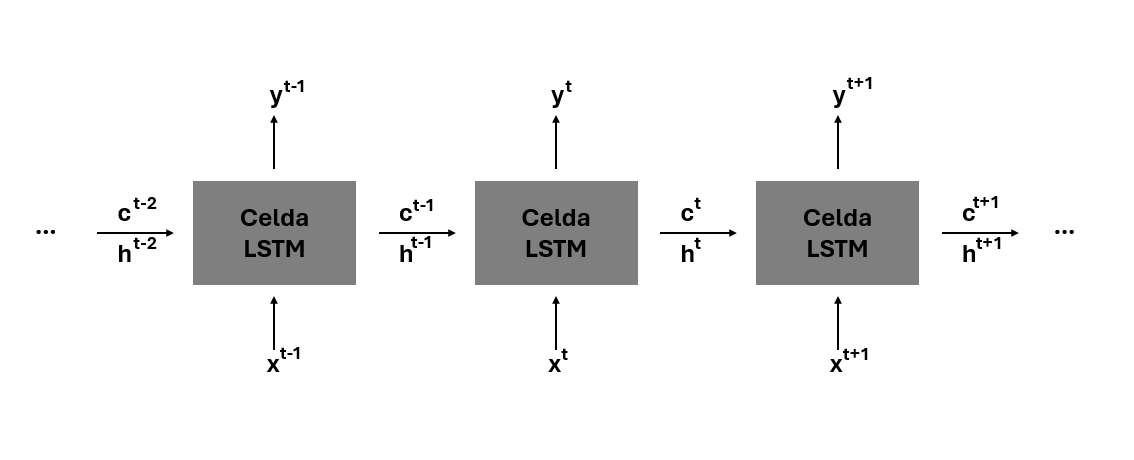
\includegraphics[width=0.55 \textwidth]{foto3.png}
    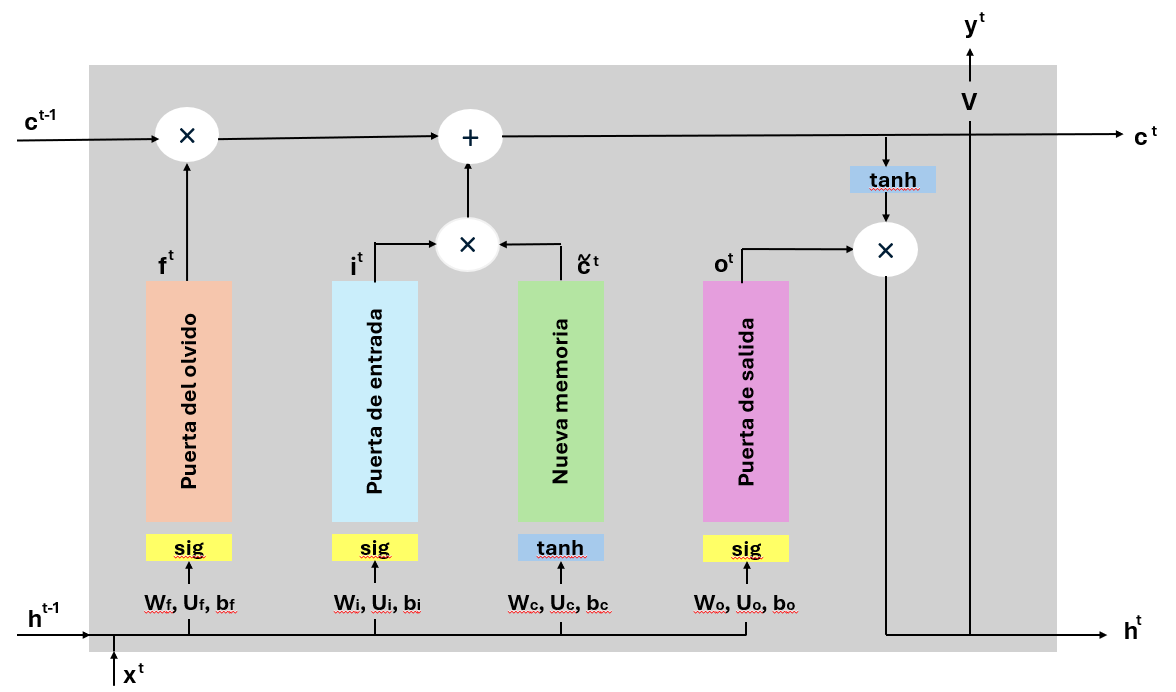
\includegraphics[width=0.55 \textwidth]{foto4.png}
    \caption{Estructura de una red LSTM desplegada en el tiempo y funcionamiento interno de una celda} 
    \label{fig:fig25}
\end{figure}


Presentan una estructura modular que consta de tres puertas (\textit{gates}) principales: la puerta de olvido (\textit{forget gate}), la puerta de entrada (\textit{input gate}), y la puerta de salida (\textit{output gate}). Estas puertas trabajan en conjunto para regular el flujo de información a través de la unidad de memoria, permitiendo un control más preciso sobre qué información retener y cuál olvidar. Se puede considerar una cuarta puerta llamada nueva celda de memoria (\textit{new memory}). Esta estructura se observa en la Figura $~\ref{fig:fig25}$

Considérese una serie temporal $\{X_t\}$ de $T$ elementos, a continuación se describe cómo llevar a cabo la propagación hacia delante. Sean $t \in \{1,...,T\}$ y $x_t$ el elemento t-ésimo de la serie temporal. Para las red LSTM, se utilizan principalmente las funciones de activación sigmoide y la tangente hiperbólica.

\vspace{0.5em}
\noindent\textnormal{\large 1. Puerta de entrada}
\vspace{0.2em}

La puerta de entrada decide cuánta nueva información debe añadirse a la memoria a largo plazo mediante una función sigmoide, generando un vector $i^{(t)} \in [0,1]^m$ que tiene por ecuación:

\begin{equation}
i^{(t)} = sig(W_ih^{(t-1)} + U_ix^{(t)} +  b_i),
\end{equation}

donde $W_i \in \mathbb{M}_{m \times m}(\mathbb{R)}, U_i \in \mathbb{M}_{m \times n}(\mathbb{R)}$ y el sesgo $b_i \in \mathbb{R}^m$ son los pesos que se aprenden para la puerta de entrada.

\vspace{0.5em}
\noindent\textnormal{\large 2. Puerta del olvido}
\vspace{0.2em}

Esta puerta determina regula cuánta información se debe olvidar y cuánta se mantiene, combinando la entrada actual y la salida anterior mediante una función sigmoide, a partir de un vector $f^{(t)} \in [0,1]^m$ que se expresa como:

 \begin{equation}
 f^{(t)} = sig(W_fh^{(t-1)} + U_fx^{(t)} +  b_f),  
 \end{equation}

donde $W_f \in \mathbb{M}_{m \times m}(\mathbb{R)}, U_f \in \mathbb{M}_{m \times n}(\mathbb{R)}$ y el sesgo $b_f \in \mathbb{R}^m$ son los pesos que se aprenden para la puerta del olvido.

\vspace{0.5em}
\noindent\textnormal{\large 3. Puerta de salida}
\vspace{0.2em}

Esta puerta determina cuánta información de la memoria actual se utilizará para la salida final, combinando la entrada actual y la información de la memoria usando una función sigmoide, mediante un vector $o^{(t)} \in [0,1]^m$ que se puede escribir como:

 \begin{equation}
 o^{(t)} = sig(W_oh^{(t-1)} + U_ox^{(t)} +  b_o),  
 \end{equation}

donde $W_o \in \mathbb{M}_{m \times m}(\mathbb{R)}, U_o \in \mathbb{M}_{m \times n}(\mathbb{R)}$ y el sesgo $b_o \in \mathbb{R}^m$ son los pesos que se aprenden para la puerta de salida.

\vspace{0.5em}
\noindent\textnormal{\large 4. Nueva celda de memoria (también conocida como \textit{block inputs})}
\vspace{0.2em}

Esta puerta considera el efecto del dato de entrada $x^{(t)} \in \mathbb{R}^n$ y el estado oculto anterior $h^{(t-1)} \in [-1,1]^m$ para representar información nueva candidata a incorporarse a la memoria, pero que debe pasar el filtro de la puerta de entrada. Esto se traduce en el vector $\tilde{c}^{(t)} \in [-1,1]^m$, que tiene por ecuación:

\begin{equation}
\tilde{c}^{(t)} = tanh(W_ch^{(t-1)} + U_cx^{(t)} +  b_c),
\end{equation}

donde $W_c \in \mathbb{M}_{m \times m}(\mathbb{R)}, U_c \in \mathbb{M}_{m \times n}(\mathbb{R)}$ y el sesgo $b_c \in \mathbb{R}^m$ son los pesos que se aprenden para la nueva celda de memoria.


Una vez se tienen las ecuaciones de las cuatro puertas, se calcula la memoria final $c^{(t)} \in \mathbb{R}^m$ de la siguiente forma:

\begin{equation}
c^{(t)} = ( f^{(t)} \circ c^{(t-1)}) + (i^{(t)} \circ \tilde{c}^{(t)}),
\end{equation}

donde $c^{(t-1)}$ es la memoria final del instante de tiempo anterior y $\circ$ representa el producto de Hadamard.

En el primer término de la suma, la puerta del olvido $f^{(t)}$ controla cuánta de la memoria anterior $c^{(t-1)}$ debe ser olvidada. Cuando más se aproxima $f^{(t)}$ a 0, más memoria se pierde de la memoria anterior. Por otro lado, la puerta de entrada $i^{(t)}$ y la nueva memoria $\tilde{c}^{(t)}$ controlan cuánta información nueva del dato de entrada se debe usar. Cuanto más se aproxima $i^{(t)}$ a $1$ y $\tilde{c}^{(t)}$ a $\pm
1$, más información nueva se usa.

Los pesos y sesgos de estas puertas se entrenan de tal manera que pasan o bloquean la entrada/información previa basada en la secuencia de entrada y el paso de tiempo en la secuencia.

Además, se calcula el nuevo estado oculto $h^{(t)} \in \mathbb{R}^m$ como:

\begin{equation}
h^{(t)} = o^{(t)} \circ tanh(c^{(t)})
\end{equation}

Finalmente, la salida $\hat{y}^{(t)} \in \mathbb{R}^p$ de la celda se obtiene como: 

\begin{equation}
\hat{y}^{(t)} = Vh^{(t)} + b_y,
\end{equation}

donde $V \in \mathbb{M}_{p \times m}$ y el sesgo $b_y \in \mathbb{R^p}$ son los pesos que se aprenden de la salida. Además, es posible aplicar una función de activación a la salida; es decir, se podría establecer $\hat{y}^{(t)} =g( Vh^{(t)} + b_y)$, con g una función de activación.


A continuación, para entrenar correctamente la red LSTM, vendría la propagación hacia atrás para actualizar los pesos y sesgos, que se lleva a cabo con el método BPTT explicado en la sección ~\ref{sec:16}, pero teniendo en cuenta ahora la estructura en puertas. Esta actualizada propagación hacia atrás, a diferencia de las RNN tradicionales, afecta en considerablemente menor medida al problema del desvanecimiento o explosión del gradiente, lo que les permite a las redes LSTM aprender dependencias de largo plazo de manera más estable.


\subsection{Predicciones con el modelo de redes LSTM}\label{sec:18}

Para finalizar este apartado de redes neuronales, se va a estudiar cómo se implementa un modelo LSTM en \textit{Python} con el paquete \textit{Keras}. En primer lugar, se describen los parámetros \cite{rnn4} principales propios de los modelos LSTM que se pueden ajustar:

\begin{itemize}
    \item \texttt{input\_size}: número de datos anteriores que se utilizan para entrenar al modelo en cada instante de tiempo.
    \item \texttt{units}: es el número de celdas LSTM en paralelo que hay en cada capa, que ayudan al aprender patrones complejos o de largo plazo. Teóricamente, se ha explicado el modelo con solo una celda, pero se puede trabajar con numerosas celdas en paralelo.
    \item \texttt{return\_sequences}: si se iguala a \textit{True}, la capa devuelve todos los estados oculto y, si se iguala a \textit{False}, solo devuelve el último estado oculto.
    \item \texttt{Dense(nº)}: este parámetro se pone al final del modelo para establecer la capa de salida. El número entre paréntesis es el número de predicciones que se desea realizar.
    \item \texttt{optimizer}: es el algoritmo que ajusta los pesos y los sesgos durante el entrenamiento. Los más comunes son \textit{adam}, \textit{rmsprop} y \textit{nadam}, que son variantes del descenso del gradiente evitan el problema del desvanecimiento/explosión del gradiente.
    \item \texttt{loss}: es la función de pérdida o coste a minimizar.
    \item \texttt{epochs}: el número de veces que se propagaga hacia delante y hacia atrás.
    \item \texttt{batch\_size}: los datos de entrenamiento se dividen en lotes (batches) para efectuarlo de manera más eficiente y que el coste computacional sea menor. El parámetro \texttt{batch\_size} indica el número de datos que habrá en cada lote.
\end{itemize}

\subsubsection{Predicciones con el modelo LSTM para el primer data set}\label{sec:19}

Se recuerda que en este conjunto de datos no se encuentran los años problemáticos del COVID. Para realizar un modelo LSTM, en primer lugar hay realizar una tarea de preprocesamiento de datos. A diferencia de los modelos clásicos, las RNN no entienden una serie temporal como una sucesión de valores, sino que requieren un formato específico para recibir los datos; esto es, por pares $(X,y)$, donde $X$ son los valores pasados (ventana temporal) e $y$ son los valores siguientes que se pretenden predecir (en nuestro caso, 1).

A continuación, se deben escalar los datos. Se hace uso del escalador \textit{MinMax} para llevarlos a un rango entre 0 y 1. Este paso es fundamental porque las redes neuronales son altamente sensibles a la escala de las variables, ya que si los datos no se escuentran escalados, el entrenamiento puede no realizarse correctamente y alterar los resultados. Además, puesto que los pesos y segos iniciales son aleatorios y se cambian cada vez que se inicializa el modelo, se fijan para que no cambien en el tiempo.

Ahora bien, para elegir los mejores parámetros para nuestro modelo LSTM, se sigue la siguiente estrategia: para cada parámetro de los explicados anteriormente, se ofrecen diversas posibilidades y se crean todas las combinaciones posibles de ellos mediante bucles anidados. Para cada combinación: se define si se trabaja con una ventana de entrada de 12 o 24 pasos de tiempo (ajustando en consecuencia el conjunto de testeo), se crean los conjuntos de entrenamiento y testeo y se reorganizan las entradas en formato adecuado para LSTM. Se contruye un modelo secuencial con dos capas ocultas y una capa de salida. Se llevaba a cabo un modelo para combinación, se entrena con el conjunto de entrenamiento y se calcula el error MSE entre las predicciones y los valores reales. Finalmente, se escoge la combinación de parámetros que minimiza el error MSE. Así, para este \textit{data set}, la mejor combinación encontrada es:

\begin{table}[ht] 
\centering
\begin{tabular}{rrrrr} 
  \hline
 \texttt{units} & \texttt{optimizer} & \texttt{epochs} & \texttt{batch\_size} & \texttt{input\_size} \\ 
  \hline
64 & \texttt{adam} & 120 & 8 & 12 \\ 
   \hline
\end{tabular}
\caption{Mejores parámetros encontrados} \label{tab:01}
\end{table}

\begin{figure}[h]
    \centering
    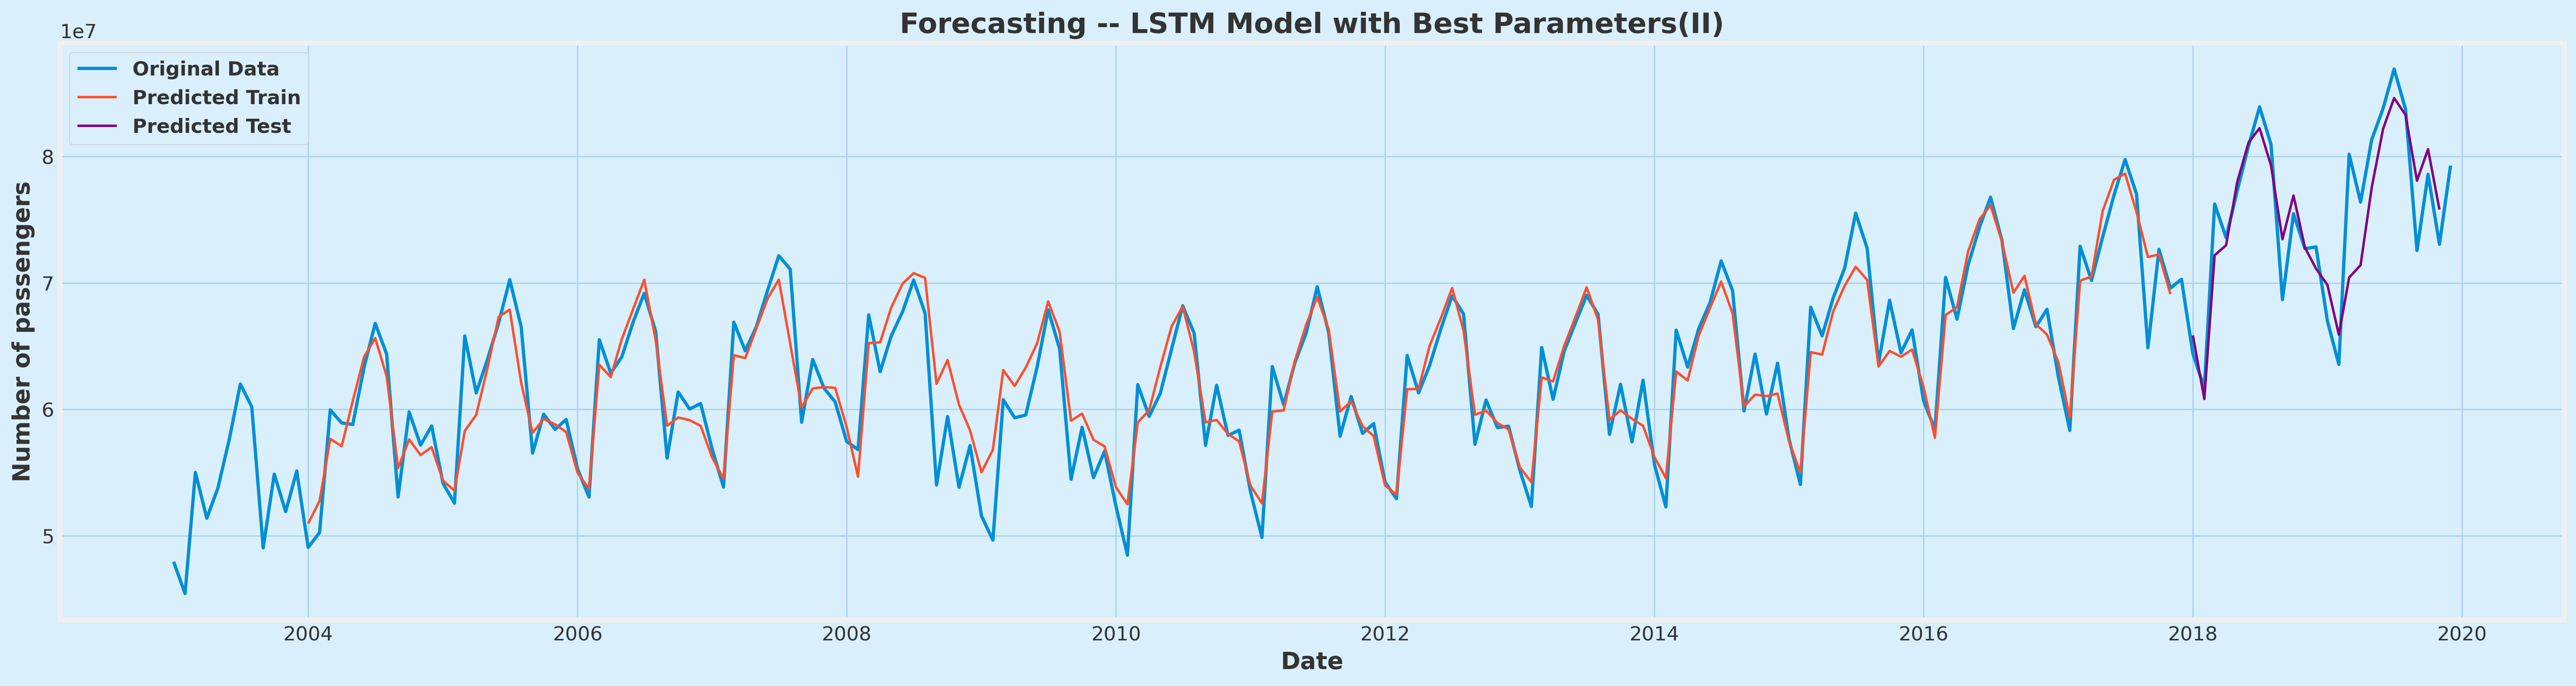
\includegraphics[width=0.9 \textwidth]{fore_best_lstm_sin_covid.png}
    \caption{Predicciones del modelo LSTM con los mejores parámetros} 
    \label{fig:fig15}
\end{figure}

%\begin{table}[h]
%\centering
%\begin{tabular}{cc}
%\hline
%\textbf{MAPE del entrenamiento} & \textbf{MAPE del testeo} \\ \hline
%2,72\% & 3,34\% \\ \hline
%\end{tabular}
%\caption{Errores MAPE del modelo LSTM}
%\label{tab:error3.1}
%\end{table}

Además, en la Figura $~\ref{fig:fig15}$ se observa que las predicciones se ajustan con bastante exactitud a los valores reales, notando que siguen las estacionalidad y patrones de los datos, a pesar de que las predicciones en ciertos momentos son menores que los valores reales. Por último, este modelo tiene un error MAPE del $3,34\%$, por lo que podemos concluir que este modelo se generaliza y adapta bien a los datos y, dado que el conjunto de entrenamiento tiene un error MAPE del $2,72\%$, podemos asegurar la no presencia de \textit{overfitting} ni \textit{underfitting}.

\subsubsection{Predicciones con el modelo LSTM para el segundo data set}\label{sec:20}

Ahora, sí se consideran los años problemáticos del COVID. Como en la subsección anterior, la primera tarea es el preprocesamiento de los datos para adecuarlos al formato que las redes neuronales requieren y la escalación de los mismos. A continuación, se eligen de la misma manera los mejores parámetros para ajustar el modelo (a partir de combinaciones de estos y que tengan el menor error MSE). Por tanto, los mejores parámetros encontrados son: 

\begin{table}[ht] 
\centering
\begin{tabular}{rrrrr} 
  \hline
 \texttt{units} & \texttt{optimizer} & \texttt{epochs} & \texttt{batch\_size} & \texttt{input\_size} \\ 
  \hline
64 & \texttt{adam} & 150 & 16 & 12 \\ 
   \hline
\end{tabular}
\caption{Mejores parámetros encontrados} \label{tab:01}
\end{table}

\begin{figure}[h]
    \centering
    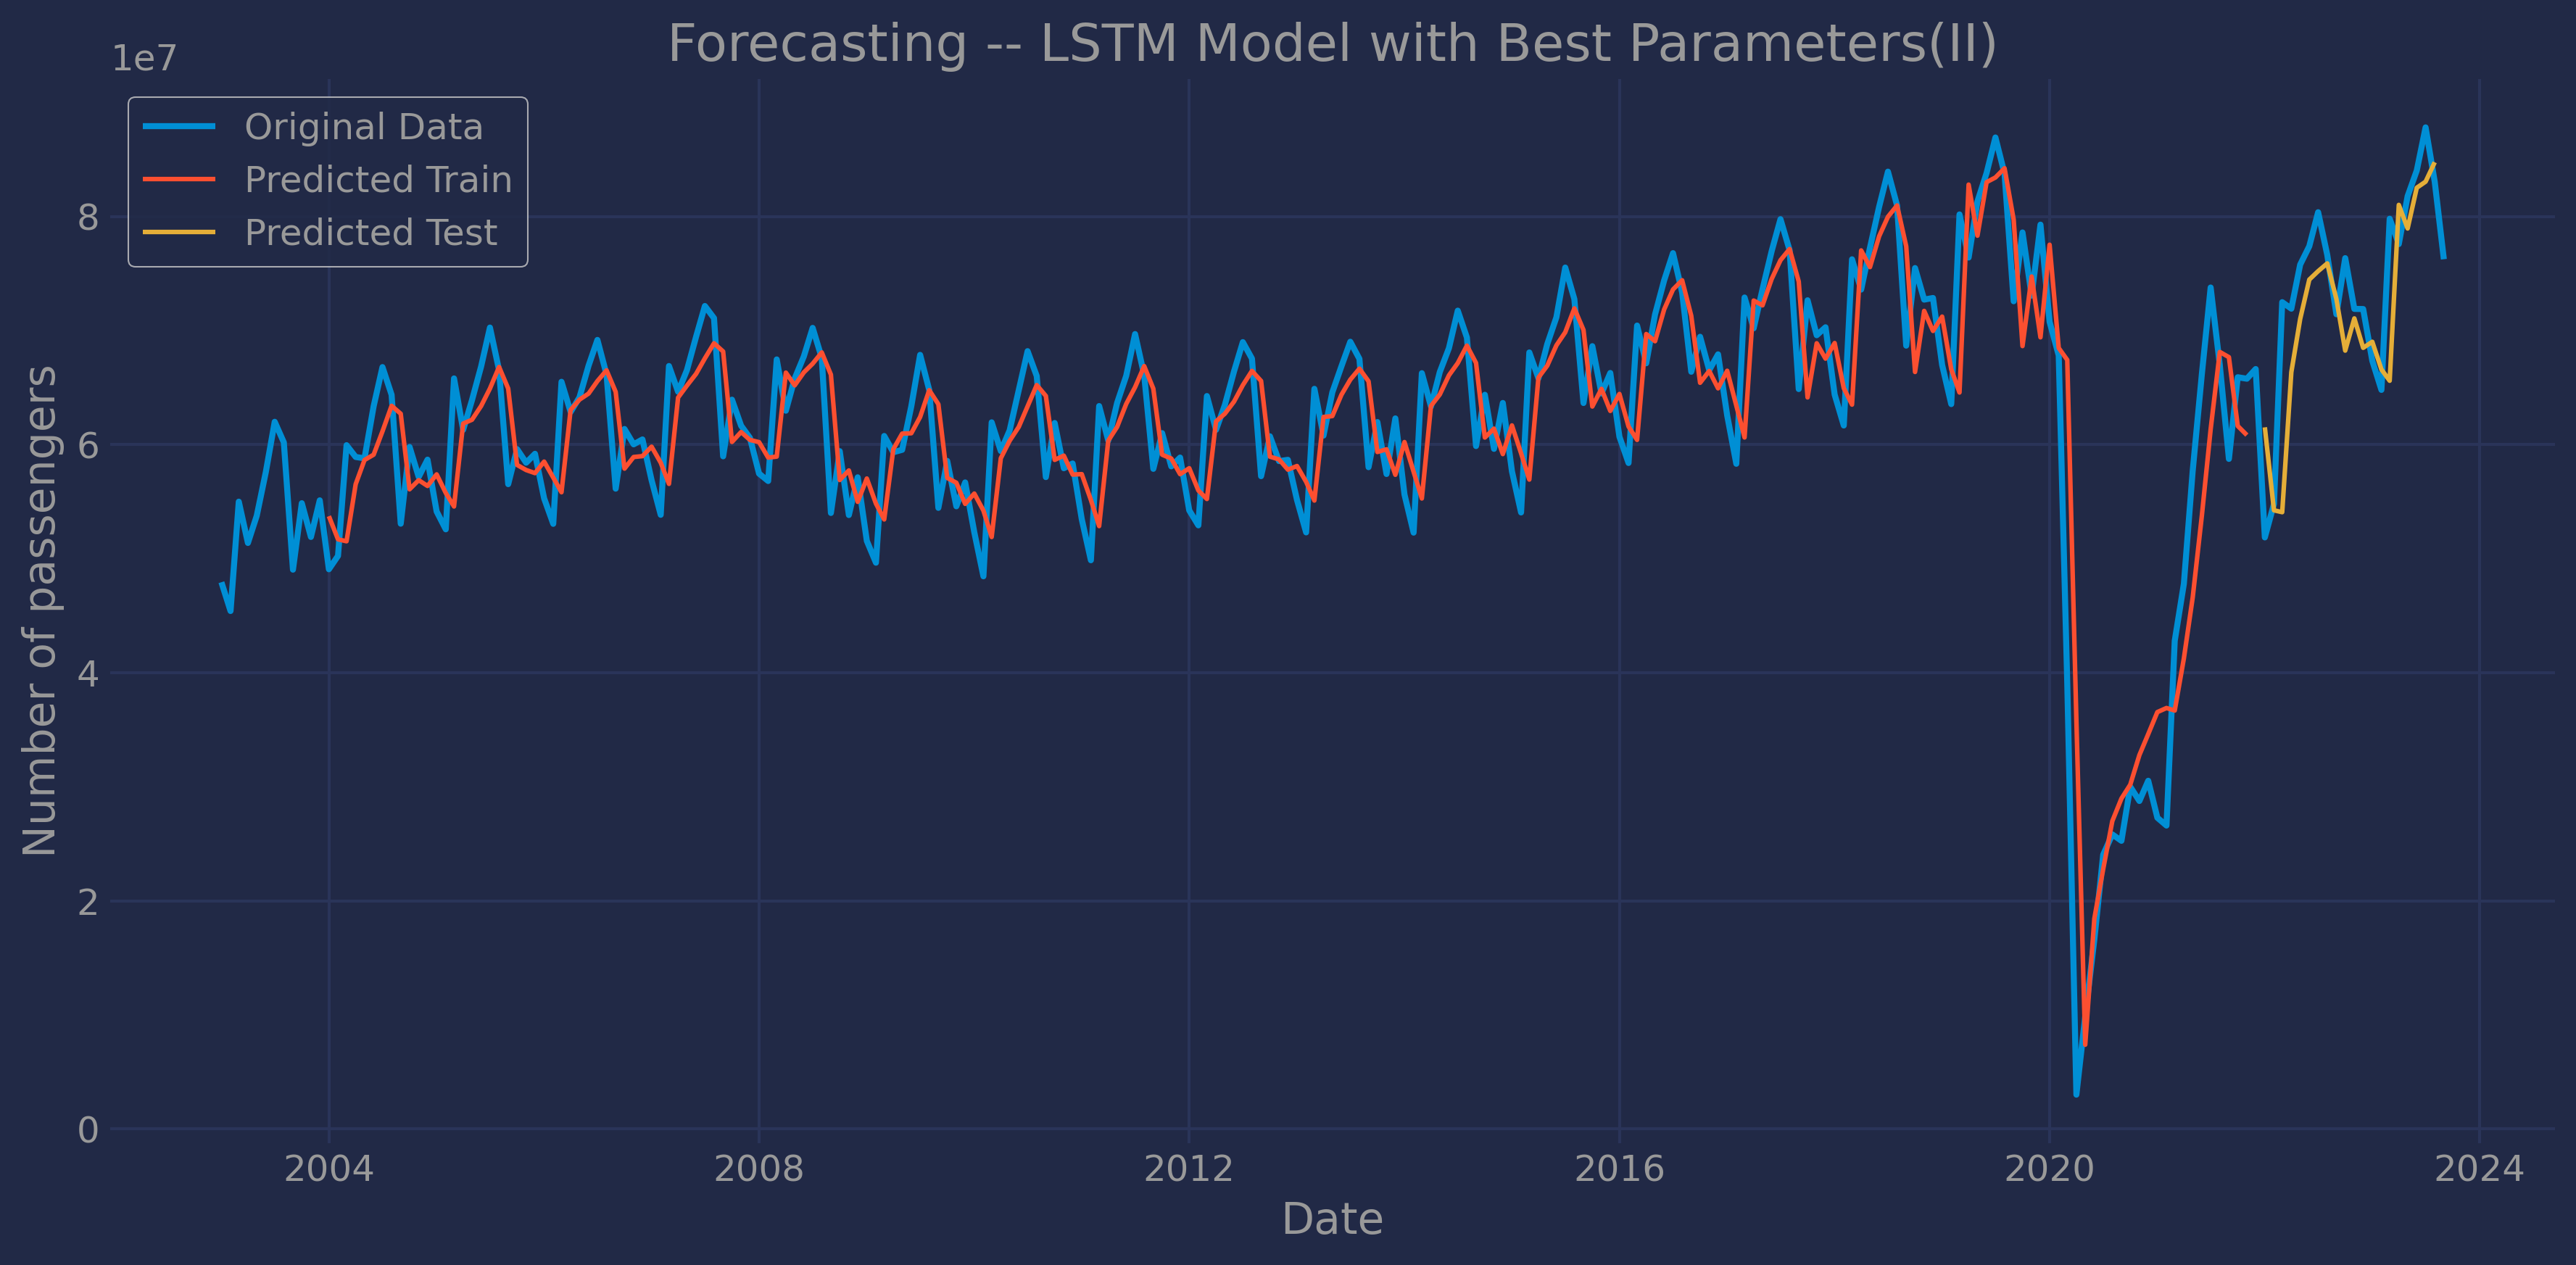
\includegraphics[width=0.9 \textwidth]{fore_best_lstm_con_covid.png}
    \caption{Predicciones del modelo LSTM con los mejores parámetrost} 
    \label{fig:fig16}
\end{figure}

%\begin{table}[h]
%\centering
%\begin{tabular}{cc}
%\hline
%\textbf{MAPE del entrenamiento} & \textbf{MAPE del testeo} \\ \hline
%12,02\% & 6,44\% \\ \hline
%\end{tabular}
%\caption{Errores MAPE del modelo LSTM}
%\label{tab:error3.2}
%\end{table}

Por consiguiente, analizando las predicciones para este modelo en la Figura $~\ref{fig:fig16}$, se aprecia que ellas se asemejan con cierta precisión a los valores reales. Teniendo en cuenta el gran impacto del COVID, el modelo se adapta rigurosamente a la tendencia que los datos siguen y mantiene los patrones de estacionalidad. Además, este modelo tiene un error MAPE del $6,44\%$, poniendo de relieve la gran capacidad de las redes neuronales a adaptarse a relaciones no lineales y cambios bruscos en los datos. El entrenamiento tiene un error MAPE del $12,02\%$, que aunque se podría intentar reducir, se encuentra en un rango aceptable. Se puede afirmar la no presencia de \textit{overfitting} ni \textit{underfitting}.

\newpage

\section{NeuralProphet}\label{sec:21}

Aunque los modelos \textit{Prophet} siguen siendo uno de los más utilizados en la predicción de series temporales, sus limitaciones como la falta de contexto local (indispensable para prever el futuro cercano) y de extensibilidad impulsaron el desarrollo de un modelo que las superara: el modelo \textit{NeuralProphet}. 

\textit{NeuralProphet} \cite{np1} es una herramienta de predicción fácil de usar e interpretable, diseñada en torno a 2021 como fusión de los componentes clásicos de series temporales introducidos por \textit{Prophet} con módulos de redes neuronales en un modelo híbrido, lo que le permite adaptarse a relaciones no lineales. 

Una de las ventajas distintivas de \textit{NeuralProphet} es su facilidad de uso. A diferencia de otras bibliotecas de aprendizaje automático, \textit{NeuralProphet} está diseñado para ser accesible incluso para aquellos sin experiencia profunda en Ciencia de Datos. Su interfaz simple y bien documentada permite a los usuarios cargar y explorar datos en series temporales, ajustar modelos y realizar predicciones en solo unas pocas líneas de código.

Al igual que en el modelo \textit{Prophet}, este modelo se puede descomponer como suma de seis componentes. Cada componente tiene sus propias entradas y procesos de modelado, aunque todas deben generar $h$ salidas, donde $h \in \mathbb{N}$ define el número de pasos que se van a predecir hacia el futuro de una sola vez. No obstante, para las explicaciones teóricas, consideraremos $h=1$. Así pues, el modelo se puede escribir como: 

\begin{equation}
\hat{y}_t = T(t) + S(t) + E(t) + F(t) + A(t) + L(t)
\end{equation}

donde:

\begin{itemize}
    \item $T(t)$ es la tendencia en el tiempo $t$.
    \item $S(t)$ son los efectos estacionales en el tiempo $t$.
    \item $E(t)$ son los efectos de eventos y festivos en el tiempo $t$.
    \item $F(t)$ son los efectos de regresión en el tiempo $t$ para variables exógenas conocidas en el futuro.
    \item $A(t)$ son los efectos de autorregresión en el tiempo $t$ basados en observaciones pasadas.
    \item $L(t)$ son los efectos de regresión en el tiempo $t$ para observaciones rezagadas de variables no objetivo.
\end{itemize}

\subsection{Tendencia}\label{sec:22}

Un enfoque clásico para modelar la tendencia siempre ha sido combinar un desplazamiento $m$ y una tasa de crecimiento $k$. \textit{NeuralProphet} utiliza este enfoque clásico, pero permite que la tasa de crecimiento cambie en distintos puntos, dando lugar a una tendencia que se modela como una serie continua por tramos lineales. Así, en una primera aproximación, podemos modelar la tendencia como: 

\begin{equation}
T(t) = \delta(t)t + \rho(t),
\label{eq:eq1}
\end{equation}

donde $\delta(t)$ es la tasa de crecimiento y $\rho(t)$ es el desplazamiento para cada momento de tiempo $t$.

Esta tendencia lineal por tramos solo varía la tasa de crecimiento de un número finito de puntos de cambios. Sin pérdida de generalidad, supongamos que esto sucede en S puntos de cambio en los tiempos $s_j$, con $j\in \{1,...,S\}$. Entre puntos de cambio, la tendencia se mantiene constante. 

Por un lado, los ajustes de tasa en cada punto de cambio se puede definir como un vector $\delta \in \mathbb{R}^S$, donde $\delta_{s_j}$ es el cambio en el j-ésimo punto de cambio. Además, la tasa de crecimiento en un instante $t$ se determina sumando a la tasa inicial $\delta_0$ la suma de los ajustes en todos los puntos de cambio hasta el tiempo $t$.

Por otro lado, el vector correspondiente a los ajustes del desplazamiento se define como $\rho \in \mathbb{R}^S$, donde $\rho_{s_j}$ es el cambio de desplazamiento en el j-ésimo punto de cambio. Sin embargo, el desplazamiento en el punto de cambio $s_j$ no es un parámetro independiente, sino que se define como $\rho_{s_j} = -c_{s_j} \delta_{s_j}$, lo que permite que la serie sea continua por tramos.

Además, introducimos un vector binario $a(t) \in \{0,1\}^S$, donde $a_j(t) = 1$ si $t\geq s_j$ y $0$ en otro caso, que representa si el tiempo $t$ ha pasado cada uno de los puntos de cambios. De esta forma, podemos reescribir la ecuación ~\ref{eq:eq1} como:

\begin{equation}
T(t) = (\delta_0 + a(t)^T \delta)t + (\rho_0 + a(t)^T\rho)
\end{equation}

Por último, \textit{NeuralProphet} posee un mecanismo semi-automático para la selección de puntos de cambio. Dado un número inicial $S$ de puntos de cambio que se pueden alcanzar, durante el entrenamiento del modelo  estos parámetros se distribuyen de forma equidistante y se pueden regularizar (para descartar aquellos que no aportan información útil). No obstante, también se puede indicar el número exacto de puntos de cambio que se desean. Así, y para evitar un sobreajuste, después del último punto de cambio se ajusta un conjunto más amplio de observaciones (por defecto, un $15\%$ de los datos de entrenamiento). Al hacer predicciones al futuro, se utiliza la última tasa de crecimiento para extrapolar linealmente la tendencia.


\subsection{Estacionalidad}\label{sec:23}

\textit{NeuralProphet} modeliza la estacionalidad usando los términos de Fourier, como se hizo originalmente en \textit{Prophet}. Entonces, para cada periodicidad $p$ (por ejemplo, $p=365,25$ para la estacionalidad lineal o $p=52,18$ para la estacionalidad semanal con datos diarios), se tiene la siguiente expresión para la estacionalidad:

\begin{equation}
S_p(t) = \sum_{n=1}^{N} \left( a_n \cdot \cos\left( \frac{2\pi n t}{p} \right) + b_b \cdot \sin\left( \frac{2\pi n t}{p} \right) \right),
\end{equation}

donde $N$ es el número de pares de términos de Fourier definidos para la estacionalidad con periodicidad $p$. Como se observa, cada término de Fourier se define como pares de funciones seno y coseno (pues permiten modelar múltiples estacionalidades). Así, para escenarios con diversas estacionalidades, se pueden definir diferentes valores de $N$ para cada estacionalidad.

Sin embargo, como cada término corresponde a una frecuencia proporcional a $\frac{n}{p}$ (se repite $n$ veces por periodicidad), conforme aumenta $n$, se incorporan oscilaciones más rápidas al patrón estacional. Así, es posible capturar tanto estacionalidades simples como complejas. No obstante, un mayor número de términos de Fourier permite al modelo ajustarse a patrones estacionales más complejos, pero demasiada flexibilidad puede llevar a un sobreajuste. Además, una vez que el modelo aprende la forma del patrón, este se repite de forma idéntica a lo largo del tiempo.

Cada estacionalidad se asocia a $2N$ coeficientes. Para cada instante de tiempo $t$, el efecto de todas las estacionalidades consideradas en el modelo se denota por $S(t)$ y se puede expresar como:

\begin{equation}
S(t) = \sum_{p \in \mathbb{P}}S_p^*(t),
\end{equation}

donde $\mathbb{P}$ es el conjunto de todas las periodicidades.

Además, se admiten tanto patrones estacionales aditivos como multiplicativos. Por consiguiente, para cada periodicidad, tenemos:

\begin{equation}
S_p^*(t) = 
\begin{cases}
T(t) \cdot S_p(t), & \text{si } S_p \text{ es multiplicativa} \\
S_p(t), & \text{en otro caso}
\end{cases}
\end{equation}

Finalmente, a la hora entrenar el modelo, \textit{NeuralProphet} decide automáticamente los tipos de estacionalidades en función de dos factores: la frecuencia de los datos (cada cuánto tiempo se tiene un dato, en nuestro caso, mensualmente) y la duración del conjunto de datos (cuánto tiempo cubren los datos en total). Para que el modelo decida activar una estacionalidad $p$, se deben satisfacer dos condiciones:

\begin{enumerate}
    \item La frecuencia de los datos debe ser más alta que la estacionalidad. Por ejemplo, si tenemos datos diarios, se podrían modelar estacionalidades semanales pero no diarias.
    \item Se tiene como mínimo dos ciclos completos de la estacionalidad. Por ejemplo, si se desea modelar una estacionalidad anual, se deben tener al menos dos años de datos.
\end{enumerate}

\subsection{Autorregresión}\label{sec:24}

La autorregresión ($AR$) hace referencia al proceso de ajustar el valor futuro de una variable a partir de sus valores pasados. El número de valores pasados $p$ incluidos se suele denominar orden del modelo $AR$, y se escribe $AR(p)$. Un modelo $AR(p)$ se suele expresar de la siguiente manera:

\begin{equation}
\hat{y}_t = c + \sum_{i=1}^p \theta_i \cdot y_{t-1}+ \epsilon_t,
\end{equation}

donde $c$ es un término de intercepto, $\epsilon_t$ es un término de ruido blanco y los $\theta_i$ son constantes tal que el polinomio característico $\phi (x)=1-\theta_1x-\theta_2x^2-...-\theta_px^p$ tiene raíces con módulo mayor que 1.

En muchas aplicaciones, el objetivo está en predecir múltiples pasos hacia al futuro. Así, llamamos horizonte y, lo denotamos por $h$, al número de predicciones realizadas a la vez. Un modelo $AR$ tradicional solo es capaz de realizar una predicción. Por ello, si se desea un horizonte $h>1$, es necesario ajustar $h$ modelos distintos. El módulo AR de \textit{NeuralProphet} se basa en una versión modificada de $AR-Net$.

$AR-Net$ es, esencialmente, un modelo autorregresivo no lineal basado en redes neuronales. Su objetivo principal es modelar las dependencias temporales a corto plazo en series temporales; es decir, cómo los valores recientes de la serie influyen directamente en el valor actual. Además, $AR-Net$ permite producir las $h$ predicciones con un solo modelo. Se utilizan las $p$ últimas observaciones de la variable objetivo $y_{t-1},y_{t-2},...,y_{t-p}$, conocidos como rezagos, como las entradas del modelo. Las salidas del modelo son $h$ valores que representan el efecto $AR$ para cada paso: $A^t(t),A^t(t+1),...,A^t(t+h-1)$. Por ejemplo, $A^t(t+2)$ representa el efecto $AR$ para la predicción $\hat{y}_{t+2}$. Por lo tanto, se tiene:

\begin{equation}
A^t(t),A^t(t+1),...,A^t(t+h-1) = AR-Net(y_{t-1},y_{t-2},...,y_{t-p})
\end{equation}

Es importante notar que cada vez que se realiza una predicción desde un origen temporal concreto, se obtienen $h$ predicciones. Así, en un tiempo dado, se pueden tener hasta $h$ predicciones diferentes, cada una originada en un momento anterior distinto. Esto refleja que, con la autorregresión, las predicciones siempre se basan en información pasada y nunca en la verdadera serie en el tiempo actual.

En la práctica, suele ser una tarea ardua encontrar el número preciso de valores pasados que se usan como entradas ($p$). Comúnmente, se suele fijar como el doble de la menor periodicidad interna o del horizonte de predicción. Otra alternativa es escoger un orden alto combinado con técnicas de regularización (~\ref{def:regularizacion}) para obtener un modelo \textit{AR} disperso. Además, el modelo \textit{AR-Net} se puede configurar de distintas formas, surgiendo así tres variantes: \textit{AR} Lineal, \textit{AR} Profundo y \textit{AR} Disperso.

\subsubsection*{1.3.1 \textit{AR} Lineal}\label{sec:25}

La configuración por defecto de \textit{AR-Net} no incluye capas ocultas y es funcionalmente idéntica a un modelo \textit{AR} clásico. Se trata de una red neuronal con una sola capa y sin función de activación (la identidad), con $p$ entradas y $h$ salidas. El modelo se puede expresar como: 

\begin{equation}
y=Wx,
\end{equation}

donde $x=(y_{t-1},y_{t-2},...,y_{t-p})$, $y=(A^t(t),A^t(t+1),...,A^t(t+h-1))$ y $W \in \mathbb{M}_{h \times p}(\mathbb{R)}$ es la matriz de pesos y cada entrada $W_{i,j}$ representa el efecto del rezago $j$ sobre el paso de predicción $i$; es decir, cuánto influye el valor pasado $y_{t-j}$ en la predicción del paso $t+i-1$.

\subsubsection*{1.3.2 \textit{AR} Profundo o \textit{Deep AR}}\label{sec:26}

Este modelo consiste en añadir capas ocultas para capturar dinámicas no lineales. En este caso, se entrena una red neuronal con un número específico de capas y dimensiones. Aunque las capas ocultas mejoran la precisión de las predicciones, estas hacen que se pierda interpretabilidad; es decir, ahora no se puede observar directamente el efecto de cada valor paso, sino que se estima su importancia a partir de los pesos absolutos en la primera capa. La arquitectura queda:

\begin{equation}
\begin{aligned}
a_1 &= f_a(W_1 x + b_1) \\
a_i &= f_a(W_i a_{i-1} + b_i), \quad \text{para } i \in \{2, \dots, l\} ,  \quad \text{con $l$ el número de capas}\\
\hat{y} &= W_{l+1} a_l
\end{aligned}
\end{equation}

donde $f_a$ es la función de acivación \textit{Relu}.


\subsubsection*{1.3.3 \textit{AR} Disperso o \textit{Sparse AR}}\label{sec:27}

\textit{AR-Net} ha probado que el orden adecuado puede aproximarse fijando un orden levemente mayor al esperado y utilizando regularización para hacer que muchos de los pesos del modelo sean 0. La función de regulación que se suele aplicar es:

\begin{equation}
\Lambda_A(\theta, \epsilon = 3, \alpha = 1) = \frac{1}{p}\sum_{i=1}^{p} \log\left(\frac{1}{3 \cdot \epsilon} + |\theta_i|\right) + \log(3) + 1
\end{equation}

donde $\theta$ representa el vector de pesos:
\begin{equation}
\theta =
\begin{cases}
W \in \mathbb{R}^{p \times h}, & \text{sin capas ocultas } (l = 0) \\
W_1 \in \mathbb{R}^{p \times d}, & \text{con capas ocultas } (l \geq 1)
\end{cases}
\end{equation}

Para concluir el efecto autorregresivo, el componente $A(t)$ viene dado por la red \textit{AR-Net}, y representa la parte de la predicción que se basa únicamente en los valores pasados de la variable objetivo.

\subsection{Regresores rezagados}\label{sec:28}

Los regresores son variables observadas de la serie temporal que se desean correlacionar con la variable objetivo. También se conocen como covariables o variables exógenas y se les llama regresores rezagados porque solo conocemos sus valores pasados. En el momento $t$ de la predicción, solo se tiene acceso a sus valores pasados observados, hasta $t-1$, siendo sus valores futuros desconocidos. Entonces, la ecuación de los regresores rezagados es la siguiente:

\begin{equation}
L(t)=\sum_{x \in \mathbb{X}}L_x(x_{t-1},x_{t-2},...,x_{t-p})
\end{equation}

Dado un conjunto de covariables $\mathbb{X} \in \mathbb{M}_{T \times m}(\mathbb{R})$, se crea un módulo de regresor rezagado por cada una de las $m$ covariables $x$, de longitud $T$. Esto permite atribuir individualmente el efecto de cada covariable en las predicciones. Cada módulo de regresor rezagado funciona de manera idéntica al módulo \textit{AR}, siendo la única diferencia las entradas. Ahora, se hacen uso de las últimas $p$ observaciones de la covariable $x$ como entradas al módulo y cada módulo produce $h$ componentes aditivos:

\begin{equation}
L_x^t(t),L_x^t(t+1),...,L_x^t(t+h-1)
\end{equation}

Estos componentes aditivos se añaden a las predicciones $\hat{y}_{t},\hat{y}_{t+1},...,\hat{y}_{t+h-1}$. Por lo tanto, se tiene:

\begin{equation}
L_x^t(t),L_x^t(t+1),...,L_x^t(t+h-1) = AR-Net(x_{t-1},x_{t-2},...,x_{t-p})
\end{equation}

Todas las consideraciones de orden, profundidad y dispersión para cada covariable son ídenticas a las del módulo \textit{AR} de la sección \ref{sec:24}, pero teniendo en cuenta el siguiente cambio: 

\begin{equation}
x = (x_{t-1},x_{t-2},...,x_{t-p}) \quad \text{; }\quad y=(L_x^t(t),L_x^t(t+1),...,L_x^t(t+h-1))
\end{equation}

Por tanto, podemos conlcuir que los efectos de regresión en el tiempo $t$ para observaciones rezagadas de variables no objetivo se expresan como:

\begin{equation}
L(t) = \sum_{x \in \mathbb{X}}L_x^t(t)
\end{equation}

\subsection{Regresores futuros}\label{sec:29}

Para modelar regresores futuros, es necesario conocer tanto sus valores pasados como sus valores futuros. Dado el conjunto de regresores futuros $\mathbb{F}\in \mathbb{M}_{T \times n_f}(\mathbb{R})$, donde $n_f$ es el número de regresores futuros, denotamos por $F(t)$ el efecto combinado de todos los regresores futuros en el instante $t$, que se expresa de la siguiente manera:

\begin{equation}
F(t) = \sum_{f\in\mathbb{F}} F^*_f(t), 
\end{equation}
 donde 
\begin{equation}
F_f^*(t) =
\begin{cases}
T(t) \cdot d_ff(t), & \text{si } f \text{ es multiplicativo} \\
d_ff(t), & \text{en otro caso}
\end{cases},
\end{equation}

con $f(t)$ el valor de la variable futura $f$ en el momento $t$ y $d_f$ el coeficiente del modelo correspondiente al regresor futuro $f\in \mathbb{F}$ (el peso que el modelo le da a esa variable). Por defecto, los regresores futuros tiene un efecto aditivo, pero también pueden configurarse para tenerlo multiplitivo sobre la tendencia.


\subsection{Eventos y festivos}\label{sec:30}

Los efectos de eventos especiales o festivos pueden ocurrir de forma esporádica. Estos efectos se modelan de forma análoga a los regresores futuros, siendo cada evento $e$ una variable binaria $e\in\{0,1\}$, que indica si el evento ocurre o no en un día determinado. Para un conjunto de eventos $\mathbb{E} \in \mathbb{M}_{T \times n_e}(\mathbb{R})$, donde $n_e$ es el número de eventos y $T$ la longitud de la serie, se denota por $E(t)$ el efecto total de todos los eventos en el instante de tiempo $t$ y se puede formular como:

\begin{equation}
E(t) = \sum_{e \in \mathbb{E}} E_e^*(t)
\end{equation}
 donde 
\begin{equation}
E_e^*(t) =
\begin{cases}
T(t) \cdot z_ee(t), & \text{si el evento } e \text{ es multiplicativo} \\
z_ee(t), & \text{en otro caso}
\end{cases},
\end{equation}

con $e(t)$ el valor del evento $e$ en el momento $t$ y $z_e$ el coeficiente del modelo correspondiente al evento $e\in \mathbb{E}$ (el peso que el modelo le da a ese evento).

Además, \textit{NeuralProphet} permite modelar dos tipos de eventos: eventos definidos por el usuario y festivos nacionales específicos de cada país. Dado un país, sus festivos se obtienen automáticamente y se añaden al conjunto de eventos $\mathbb{E}$. Al igual que ocurre con los regresores futuros, los eventos también pueden definirse como aditivos o multiplicativos.

Por último, para un evento que ocurre en el tiempo $t_e$, se puede definir una ventana $[t_e-i,t_e+j]$ de $i+j$ días que se consideren eventos especiales por sí mismos. Por ejemplo, al establecer una ventana de $[-1,0]$ para Navidad, se permite que el día anterior a Navidad tenga su propio efecto en la predección. De este modo, se crea una variable para cada día dentro de la ventana alrededor del evento, y se añade al conjunto de eventos $\mathbb{E}$. 


\subsection{Predicciones con el modelo \textit{NeuralProphet}}\label{sec:31}

Para ultimar la sección de \textit{NeuralProphet}, se van a estudiar las predicciones para este modelo. Una de las diferencias fundamentales entre \textit{Prophet} y \textit{NeuralProphet} es el procedimiento de ajuste. Prophet usa L-BFGS y está implementado en \textit{Stan}, mientras que \textit{NeuralProphet} utiliza \textit{PyTorch} y entrenamiento mediante descenso de gradiente estocástico (SGD), lo que lo hace más flexible y escalable.

Al igual que para \textit{Prophet}, se pueden ajustar manualmente numerosos hiperparámeteros \cite{np2} en \textit{Python}:

Para la tendencia, con el parámetro \texttt{trend\_reg} (que por defecto es $0$) se puede controlar la regularización de la tendencia; es decir, penalizar cambios bruscos o forzar que los cambios de pendiente sean pequeños. Un valor alto supone la evasión de cambios bruscos, mientras que un valor pequeño permite cambios de pendiente mayores. Además, se puede definir un umbral mínimo para que solo los cambios de pendiente mayores que dicho umbral sean penalizados, con el parámetro \texttt{trend\_reg\_treshold} y cuyo valor por defecto es $0,01$.

En cuanto a la estacionalidad, se puede elegir entre estacionalidad anual, semanal y diaria (o elegir varias), con los parámetros \texttt{yearly\_seasonality}, \texttt{weekly\_seasonality} y \texttt{daily\_seasonality}, respectivamente. No tienen un valor \texttt{True} o \texttt{False} por defecto, ya que depende de la cantidad de datos de los que se dispone. También, se puede decidir entre una estacionalidad aditiva o una multiplicativa, con \texttt{seasonality\_mode}, que por defecto es aditiva.

Por su parte, para la autorregresión, se establece el número de rezagos que el modelo debe considerar con el parámetro \texttt{n\_lags}, que por defecto es $0$. Es recomendable que este parámetro sea mayor que \texttt{n\_forecasts}, que es el horizonte de predección, por defecto $1$.

Por otro lado, para los eventos o festivos, se pueden incluir los mismos a través del parámetro \texttt{add\_events}. Asimismo, se pueden incluir automáticamente los festivos de un país con \texttt{add\_country\_holidays}.

Además, se pueden añadir regresores (variables exógenas) con los parámetros 
\newline
\texttt{add\_future\_regressor} (para incluir regresores conocidos en el futuro y cuyos valores futuros serán necesarios para el modelo) y \texttt{add\_lagged\_regressor} (para incluir regresores que solo se conocen en el pasado).

En lo que respecta a la parte de redes neuronales, también se pueden ajustar los parámetros \texttt{ar\_layers}, que define el número de capas ocultas y sus tamaños para \textit{AR-Net} en el modelo general, y \texttt{lagged\_reg\_layers}, que define el número de capas ocultas y sus tamaños para los regresores retrasados en el modelo global.


Asimismo, para el entrenamiento, se ajustan:

\begin{itemize}
    \item El número de épocas del entrenamiento con \texttt{epochs}. Si no se especifican, se determinan como 
    \begin{equation}
    N_{\text{epoch}}^* = \frac{1000 \cdot 2^{\frac{5}{2} \log_{10}(T)}}{T}
    \quad \text{ ; } \quad
    N_{\text{epoch}} = \min\left( 500, \max\left( 50, \left\lfloor N_{\text{epoch}}^* \right\rfloor \right) \right)
    \end{equation}
    \item La función de pérdida o penalización con \texttt{loss\_func}. Por defecto, se utiliza la función de Huber: 
    \begin{equation}
    L_{\text{huber}}(y, \hat{y}) =
    \begin{cases}
    \frac{2}{\beta} (y - \hat{y})^2, & \text{si } |y - \hat{y}| < \beta \\
    |y - \hat{y}| - \frac{2}{\beta}, & \text{en otro caso}
    \end{cases}
    \end{equation}
    \item El optimizador con \texttt{optimizer}. Por defecto, se hace uso de AdamW.
    \item La tasa de aprendizaje con \texttt{learning\_rate}. Por defecto, se elige la tasa donde el descenso del gradiente es más pronunciado. Se repite el test 3 veces y se hace la media logarítmica: 
    \begin{equation}
    \eta^* = \frac{1}{3} \left( \log_{10}(\eta_1) + \log_{10}(\eta_2) + \log_{10}(\eta_3) \right) \quad \Rightarrow \quad \eta = 10^{\eta^*}
    \end{equation}
    \item El número de lotes en que se agrupan los datos con \texttt{batch\_size}. Si no se especifica, se obtiene como: 
    \begin{equation}
    B^* = 2^{\left\lfloor \log_{10}(T) \right\rfloor}
    \quad \text{ ; } \quad
    B = \min\left( T, \max\left( 16, \min\left( 256, B^* \right) \right) \right)
    \end{equation}
\end{itemize}


\subsubsection{Predicciones con el modelo \textit{NeuralProphet} para el primer \textit{data set}}\label{sec:32}

\begin{figure}[h]
    \centering
    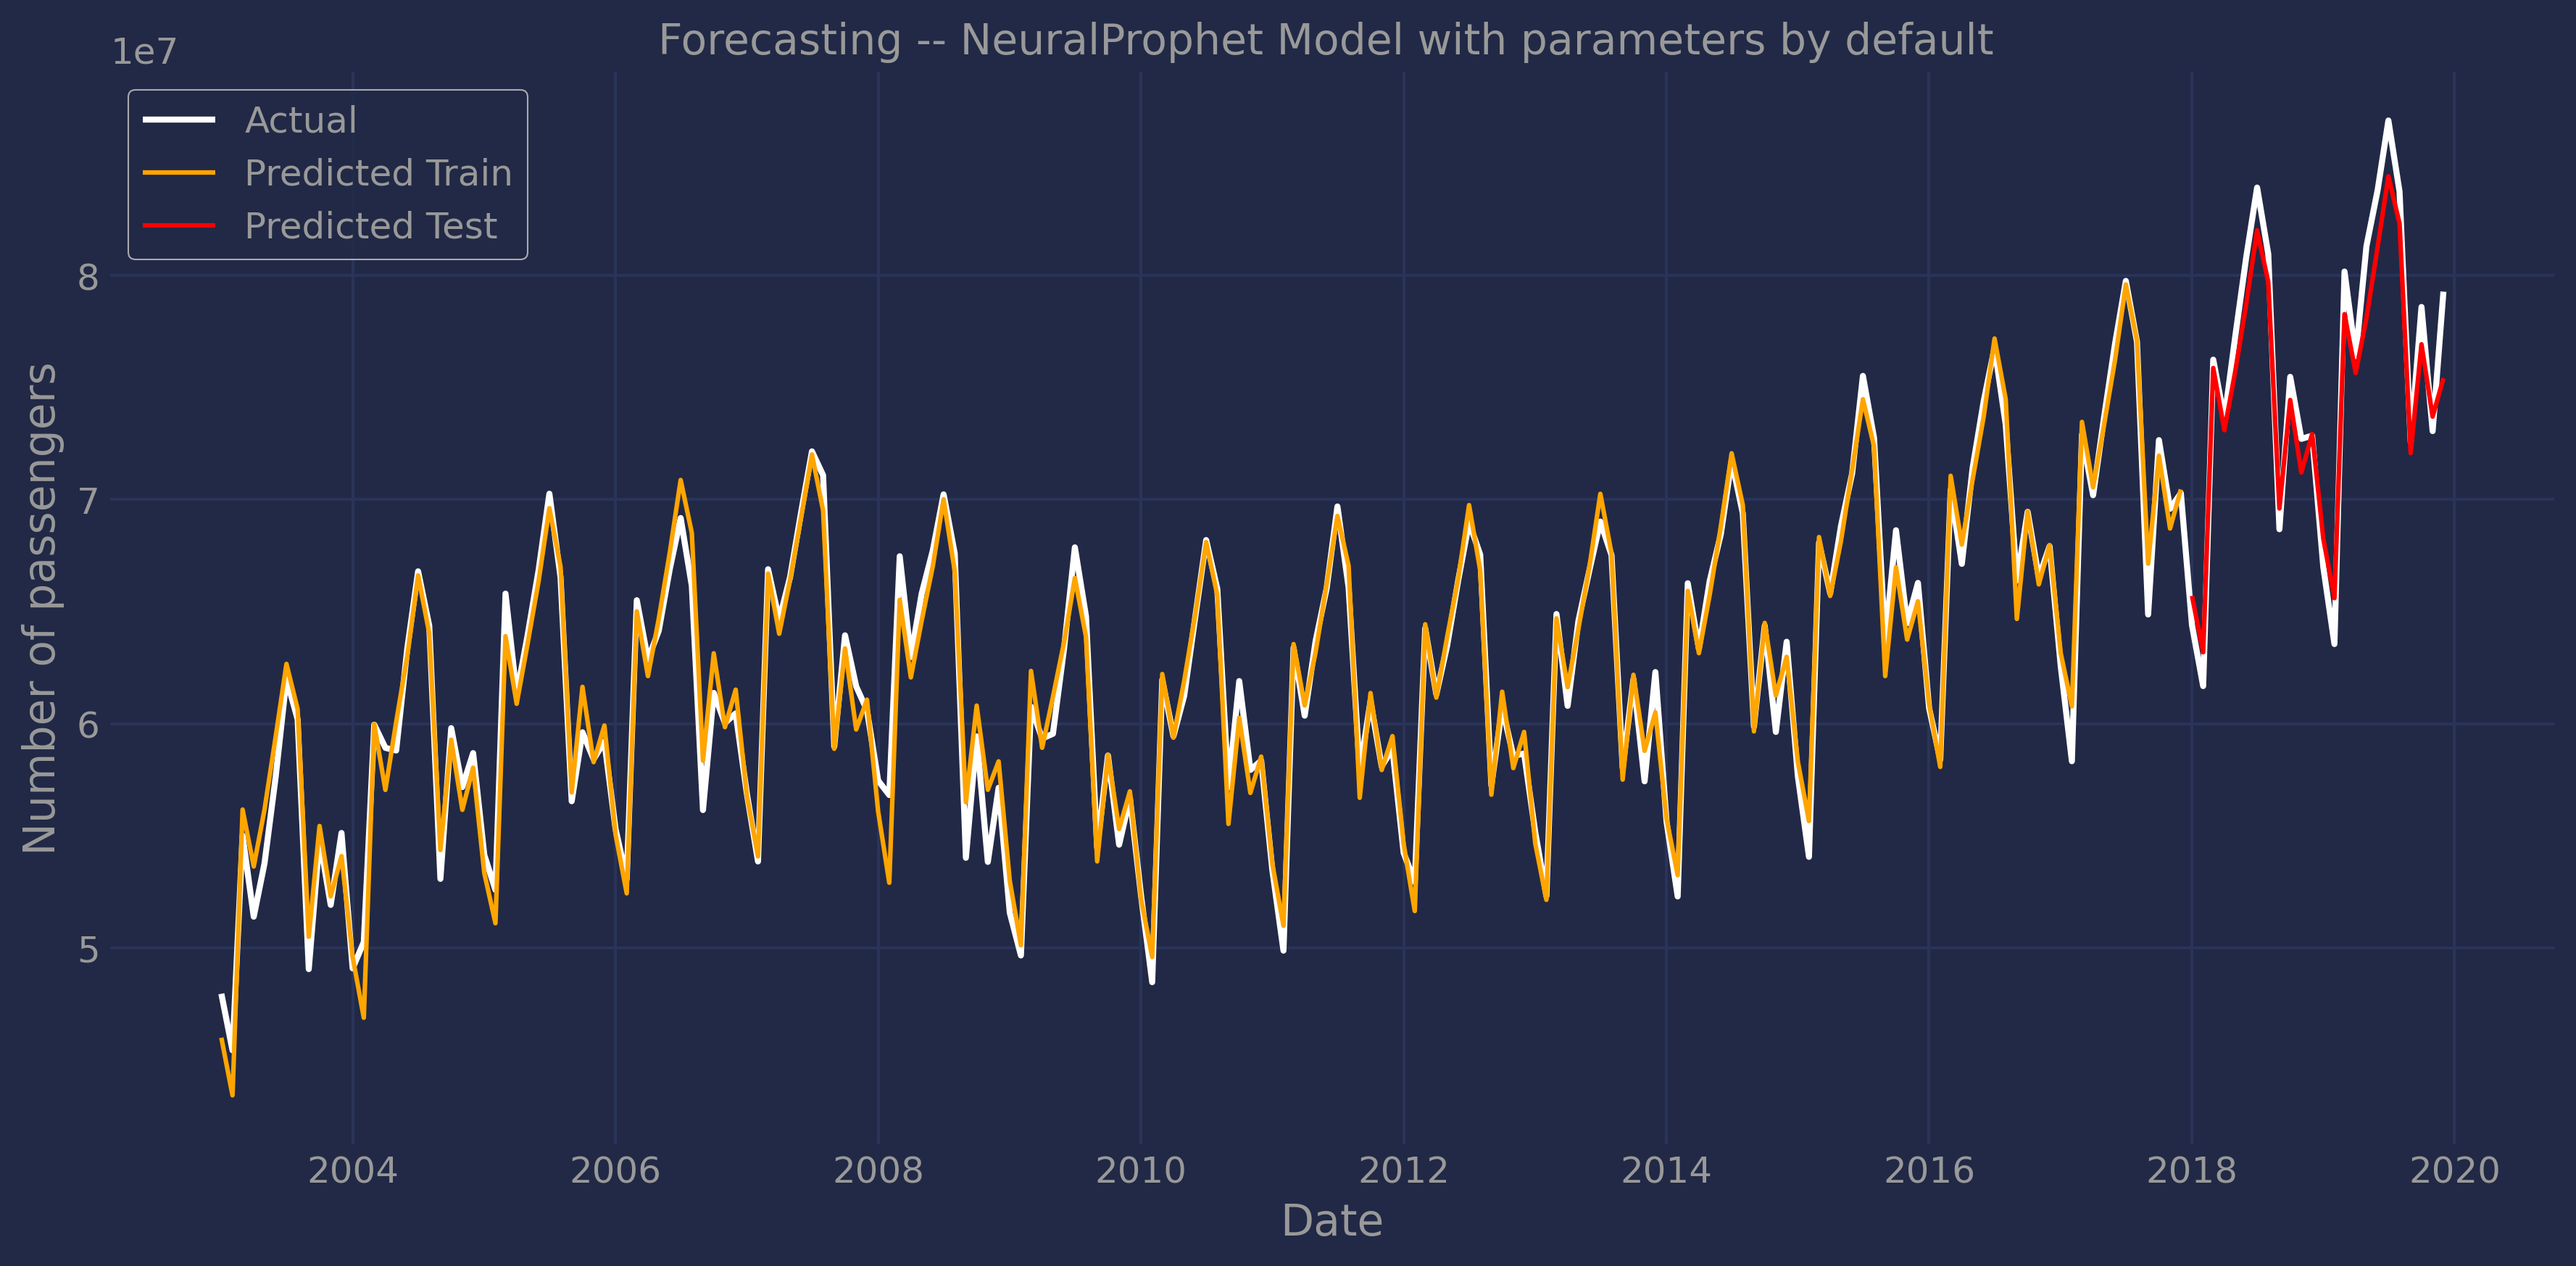
\includegraphics[width=0.8\textwidth]{default_sin_covid.png}
    \caption{Predicciones del modelo \textit{NeuralProphet} con parámetros por defecto} 
    \label{fig:fig17}
\end{figure}

Para una primera aproximación, se lanza un modelo con los valores por defecto, sin añadir regresores ni festivos. Como se puede ver en la Figura $~\ref{fig:fig17}$, el modelo se ajusta adecuadamente a la tendencia de la datos, además de seguir los mismos patrones de estacionalidad. Así, al predicir para los años 2018-2019 (años del conjunto de testeo), se presenta un error MAPE del $1,98\%$.

Ahora, se propone un nuevo modelo pero intentando escoger los mejores parámetros. Para cada parámetro de los explicados anteriormente, se ofrecen diversas posibilidades y se crean todas las combinaciones posibles de ellos. Se llevaba a cabo un modelo para combinación y se entrena con el conjunto de entrenamiento y se calcula el error MSE entre las predicciones y los valores reales. Finalmente, se escoge la combinación de parámetros que minimiza el error MSE. Sin embargo, dada la cantidad de parámetros que hay para ajustar, el tiempo de computación se puede alargar horas y horas, por lo que se ha optado por realizar una búsqueda aleatoria sobre 200 muestras. Por ello, se escoge la mejor combinación de hiperparámetros y se parte de ellos para encontrar la combinación que menor error MAPE genere.

\begin{figure}[h]
    \centering
    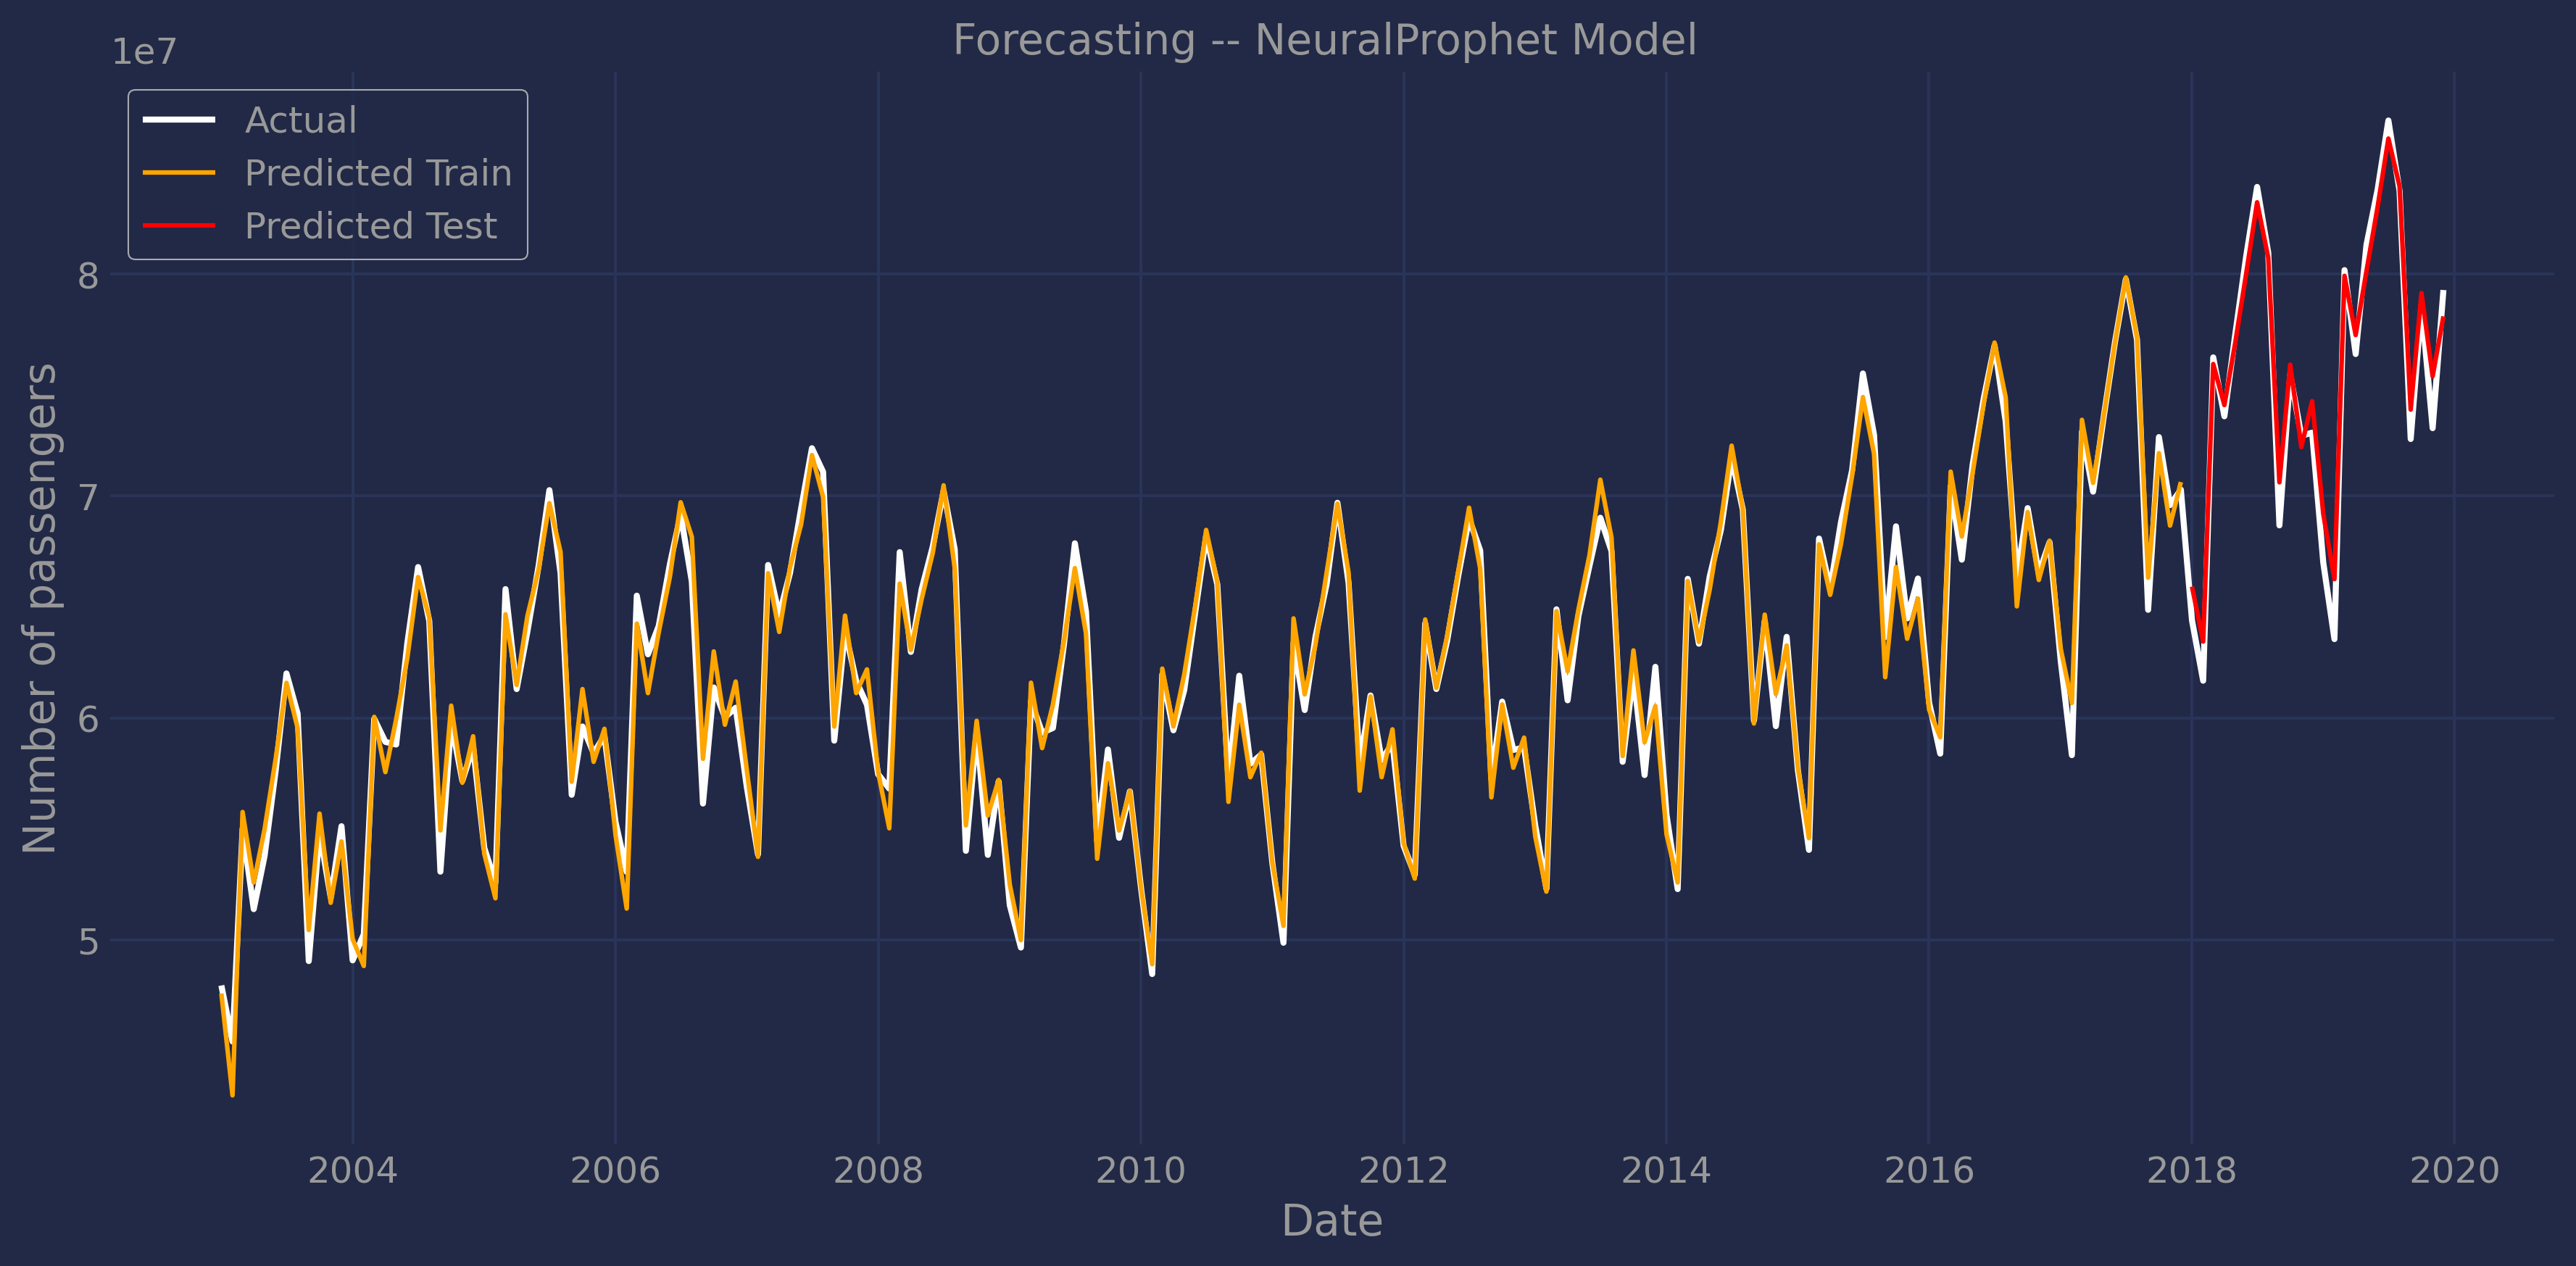
\includegraphics[width=0.8\textwidth]{best_sin_covid.png}
    \caption{Predicciones del segundo modelo \textit{NeuralProphet}} 
    \label{fig:fig18}
\end{figure}

Así, modificando parámetros utilizando la estrategia anterior, se llega a la combinación siguiente: el número de épocas a 1000 y añadir como regresor futuro el número total de vuelos, el resto de parámetros se toma por defecto. Se pueden ver las predicciones de este nuevo modelo en la Figura $~\ref{fig:fig18}$ y se nota que, de nuevo, el modelo se adecúa a los datos ya que se siguen los patrones estacionales y la tendencia. Además, se obtiene un error MAPE del $1,44\%$.

\begin{table}[h]
\centering
\begin{tabular}{ccc}
\hline
\textbf{Modelo} & \textbf{MAPE del entrenamiento} & \textbf{MAPE del testeo} \\ \hline
\text{Con valores por defecto} & 1,34\% & 1,98\% \\ \hline
\text{Con los mejores parámetros} & 1,11\% & 1,44\% \\ \hline
\end{tabular}
\caption{Errores MAPE del modelo NeuralProphet}
\label{tab:error4.1}
\end{table}

En la Tabla $~\ref{tab:error4.1}$, se ven los errores MAPE de ambos modelos para el entrenamiento y el testeo. Ambos modelos son bastante buenos, pues presentan errores pequeños. Sin embargo, el segundo modelo presenta una sutil mejora con respecto al primero, por lo que este es el modelo elegido. Además, se observa que ninguno de los modelos cae en \textit{overfitting} ni \textit{underfitting}.

\begin{figure}[h]
    \centering
    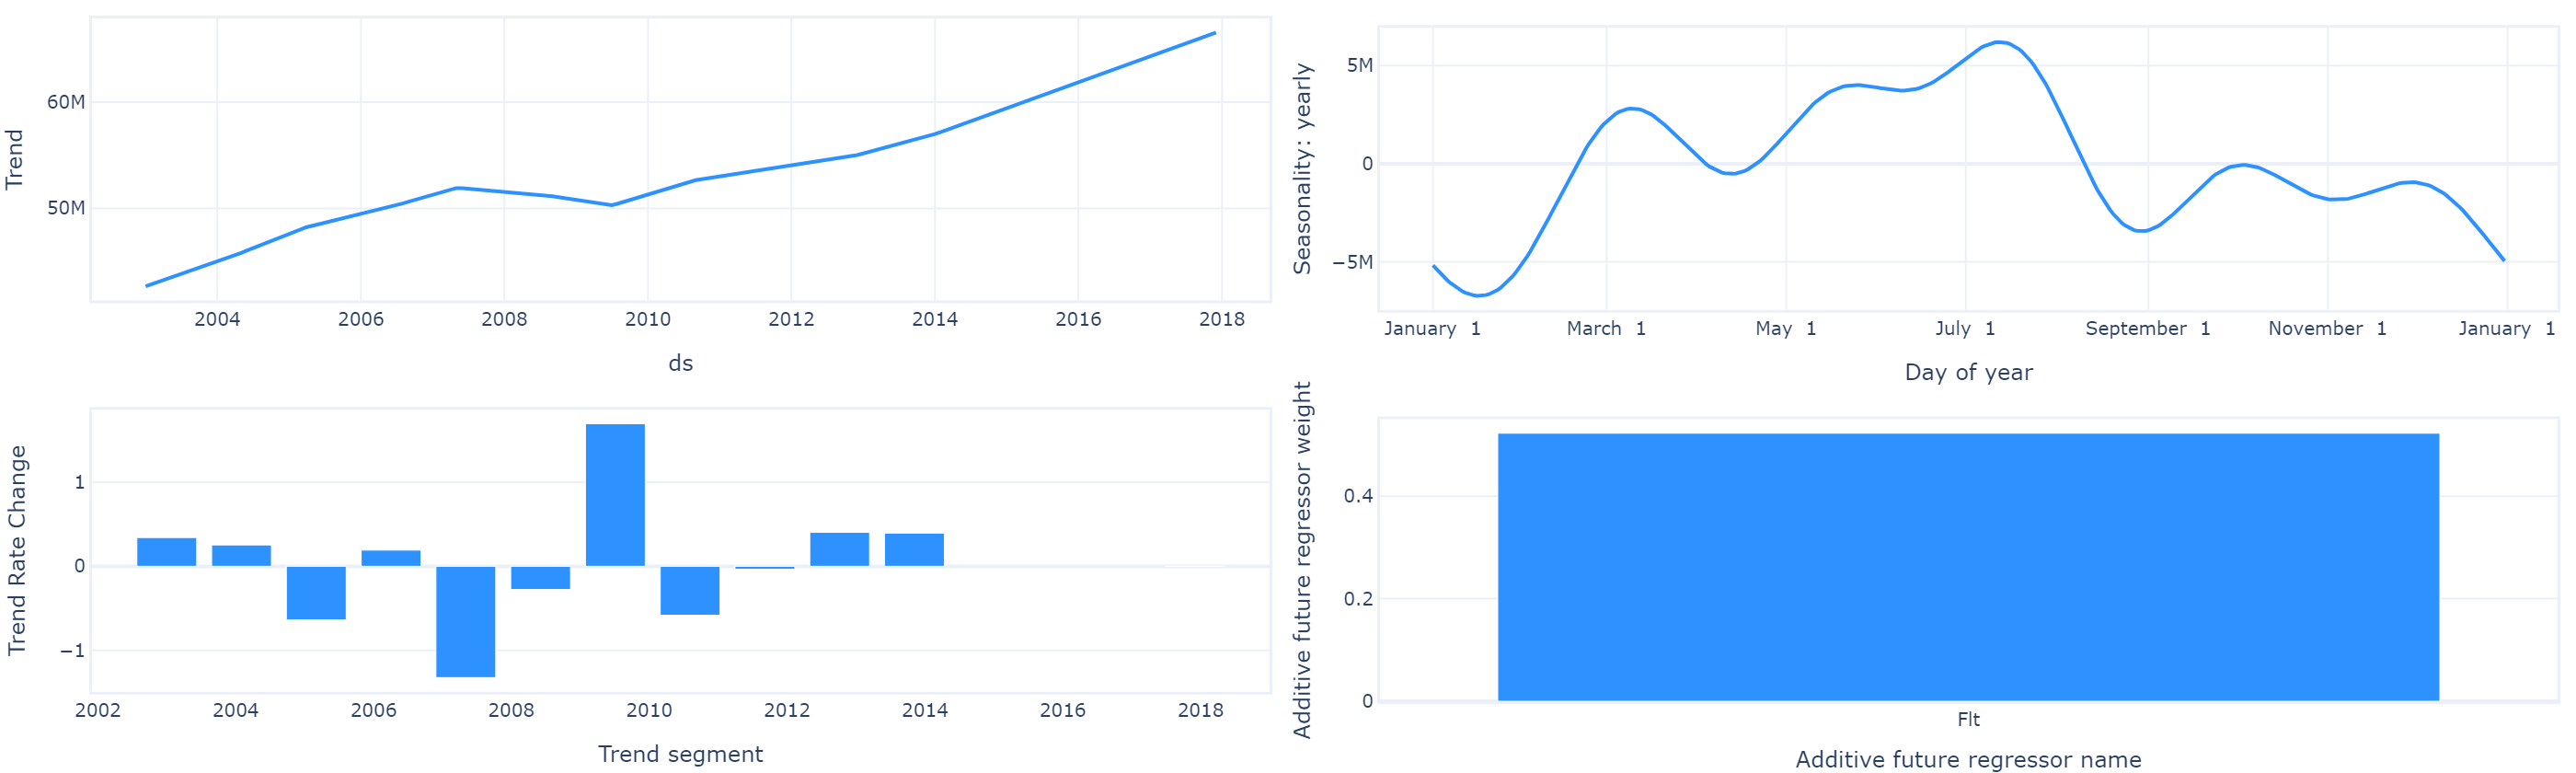
\includegraphics[width=0.8\textwidth]{best_params_sin_covid_dividida.png}
    \caption{Parámetros del mejor modelo \textit{NeuralProphet}} 
    \label{fig:fig19}
\end{figure}

Finalmente, para este modelo, se observa en la Figura $~\ref{fig:fig19}$ el comportamiento de ciertas componentes: para la tendencia, se tiene un claro crecimiento entre 2003 y 2018, con ligeros descensos en 2009 y 2011, generados probablemente por la crisis económica de dichos años. Los cambios de tasa de tendencia muestran el cambio de la pendiente de la tendencia en cada segmento. En general, los cambios no son muy abruptos salvo que en 2008-2009, donde se observa una clara caída, seguida de un fuerte aumento en 2010. Para la estacionalidad anual, se notan picos entre mayo-julio (verano) y mínimos en enero y octubre (invierno y principios de otoño), comportamiento coherente para el tráfico aéreo de pasajeros. Finalmente, para el regresor futuro, se aprecia que tiene un impacto significativo y positivo en la predicción del número de pasajeros.


\subsubsection{Predicciones con el modelo \textit{NeuralProphet} para el segundo \textit{data set}}\label{sec:33}

\begin{figure}[h]
    \centering
    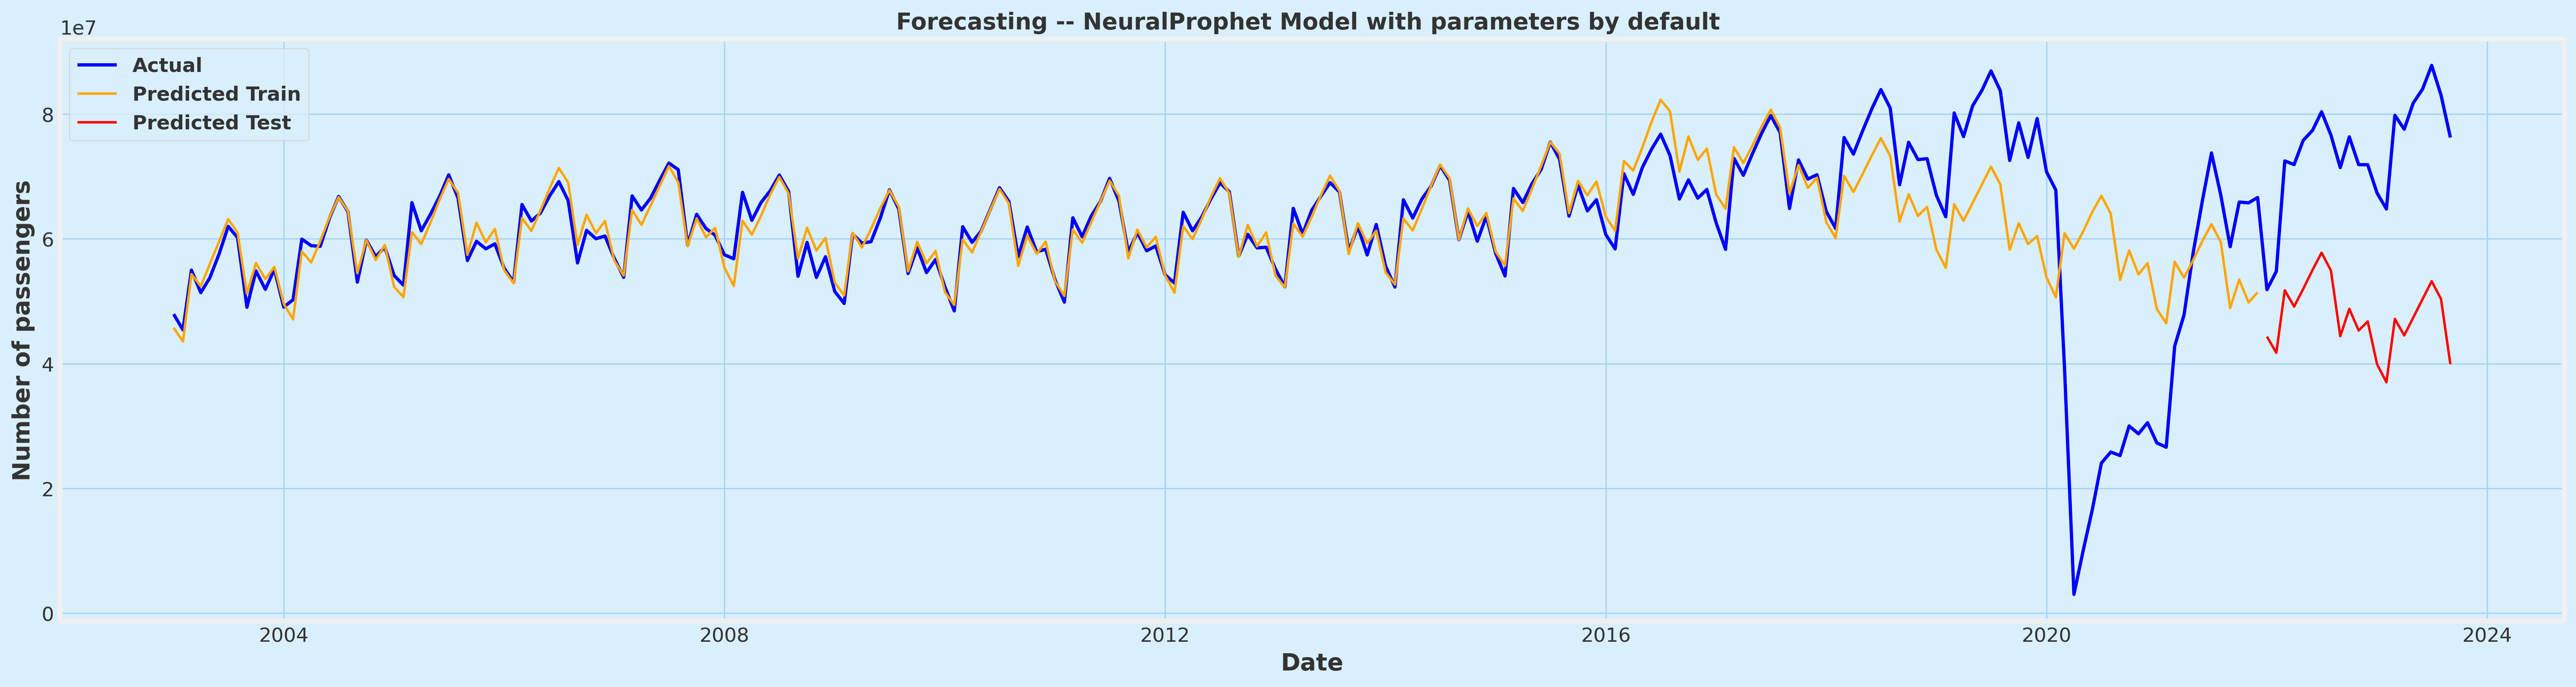
\includegraphics[width=0.9\textwidth]{default_con_covid.png}
    \caption{Predicciones del modelo \textit{NeuralProphet} con parámetros por defecto} 
    \label{fig:fig20}
\end{figure}

De nuevo, se comienza con un modelo \textit{NeuralProphet} exclusivamente con valores por defecto, sin añadir festivos ni regresores. Así, en la figura $~\ref{fig:fig20}$, se ve que al principio el modelo se adecúa con exactitud a los datos; pero, a partir 2019, comienza a desajustarse por completo y desemboca en una tendencia totalmente diferente a la que es: desde 2022 hasta 2024, el número de pasajeros empieza a aumentar lentamente, pero el modelo capta que sigue disminuyendo. No obstante, la estacionalidad se mantiene. Además, este modelo tiene un error MAPE del $35,05\%$ para los años 2022-2023 (años del conjunto de testeo).

\begin{figure}[h]
    \centering
    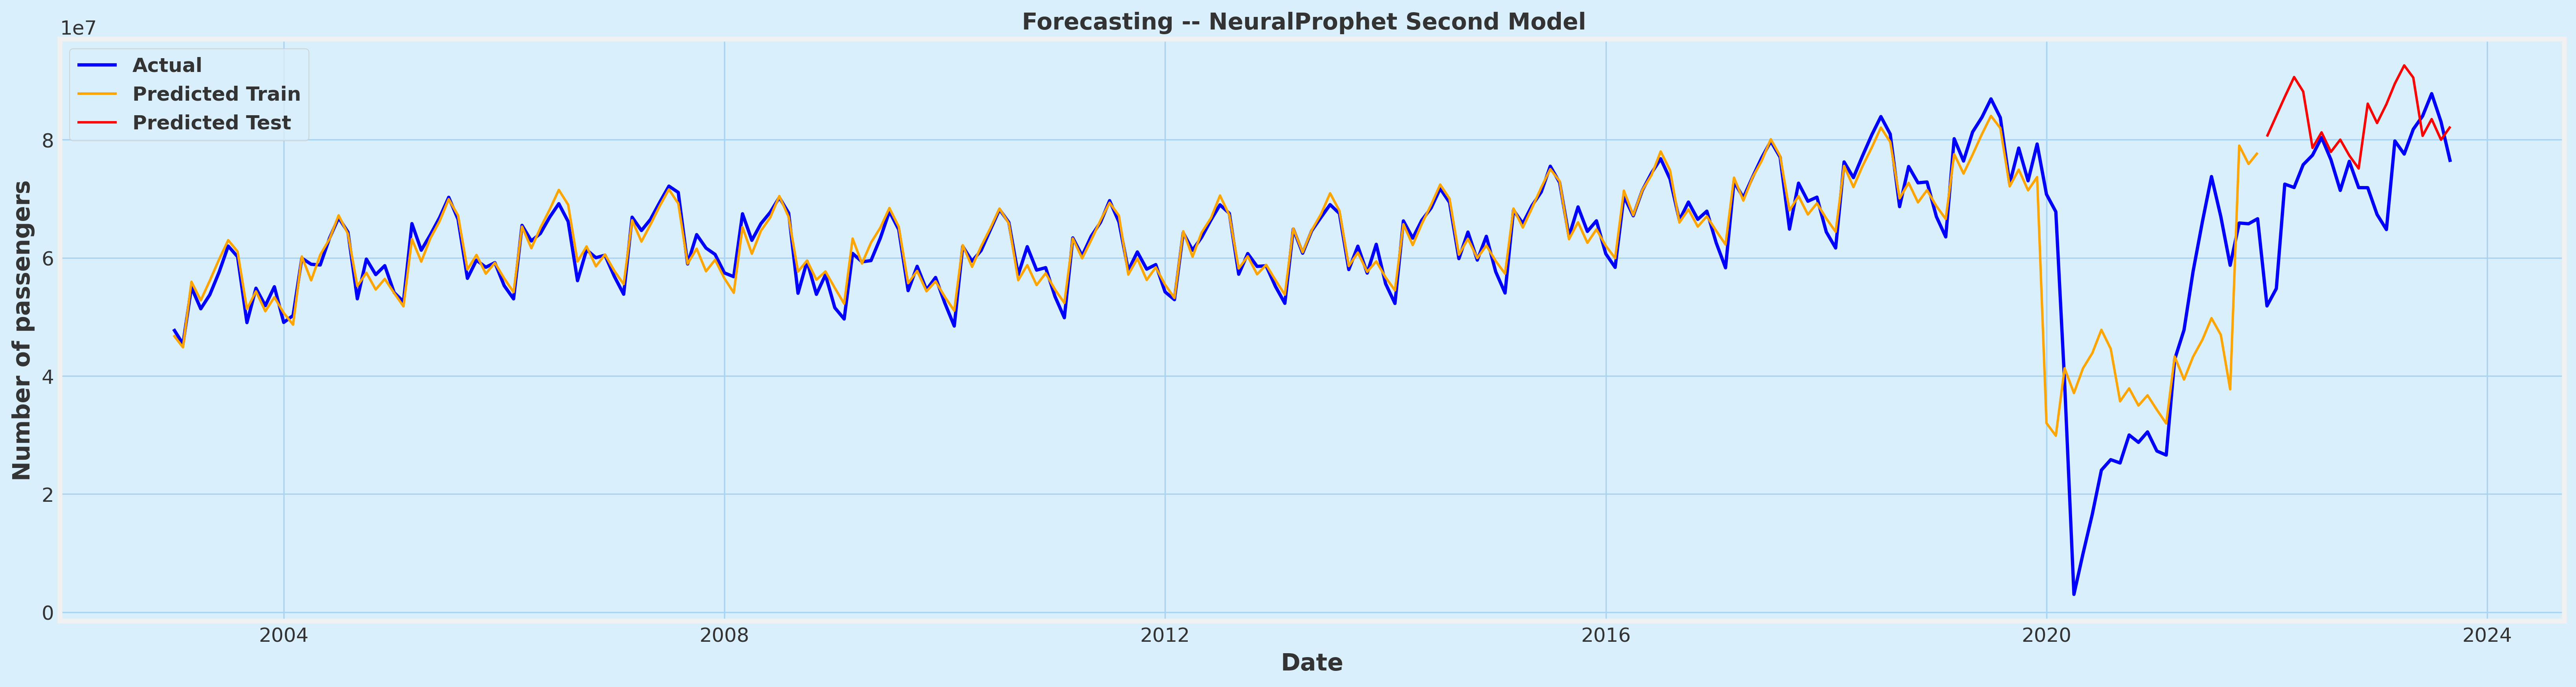
\includegraphics[width=0.8\textwidth]{second_con_covid.png}
    \caption{Predicciones del modelo \textit{NeuralProphet} con parámetros por defecto y festivos} 
    \label{fig:fig21}
\end{figure}

Para tratar de mejorar este modelo, se propone el mismo pero añadiéndole los festivos, que en este caso son la época del COVID (desde enero de 2020 hasta septiembre de 2021). Por tanto, en la Figura $~\ref{fig:fig21}$ se observa que ahora se le ha restado importancia a la época de COVID, pues el modelo se adapta considerablemente mejor a los datos. Sin embargo, se nota que se le ha restado demasiada importancia, pues las predicciones son mayores que los datos reales. Además, el modelo nuevo presenta un error MAPE del $15,81\%$.

\begin{figure}[h]
    \centering
    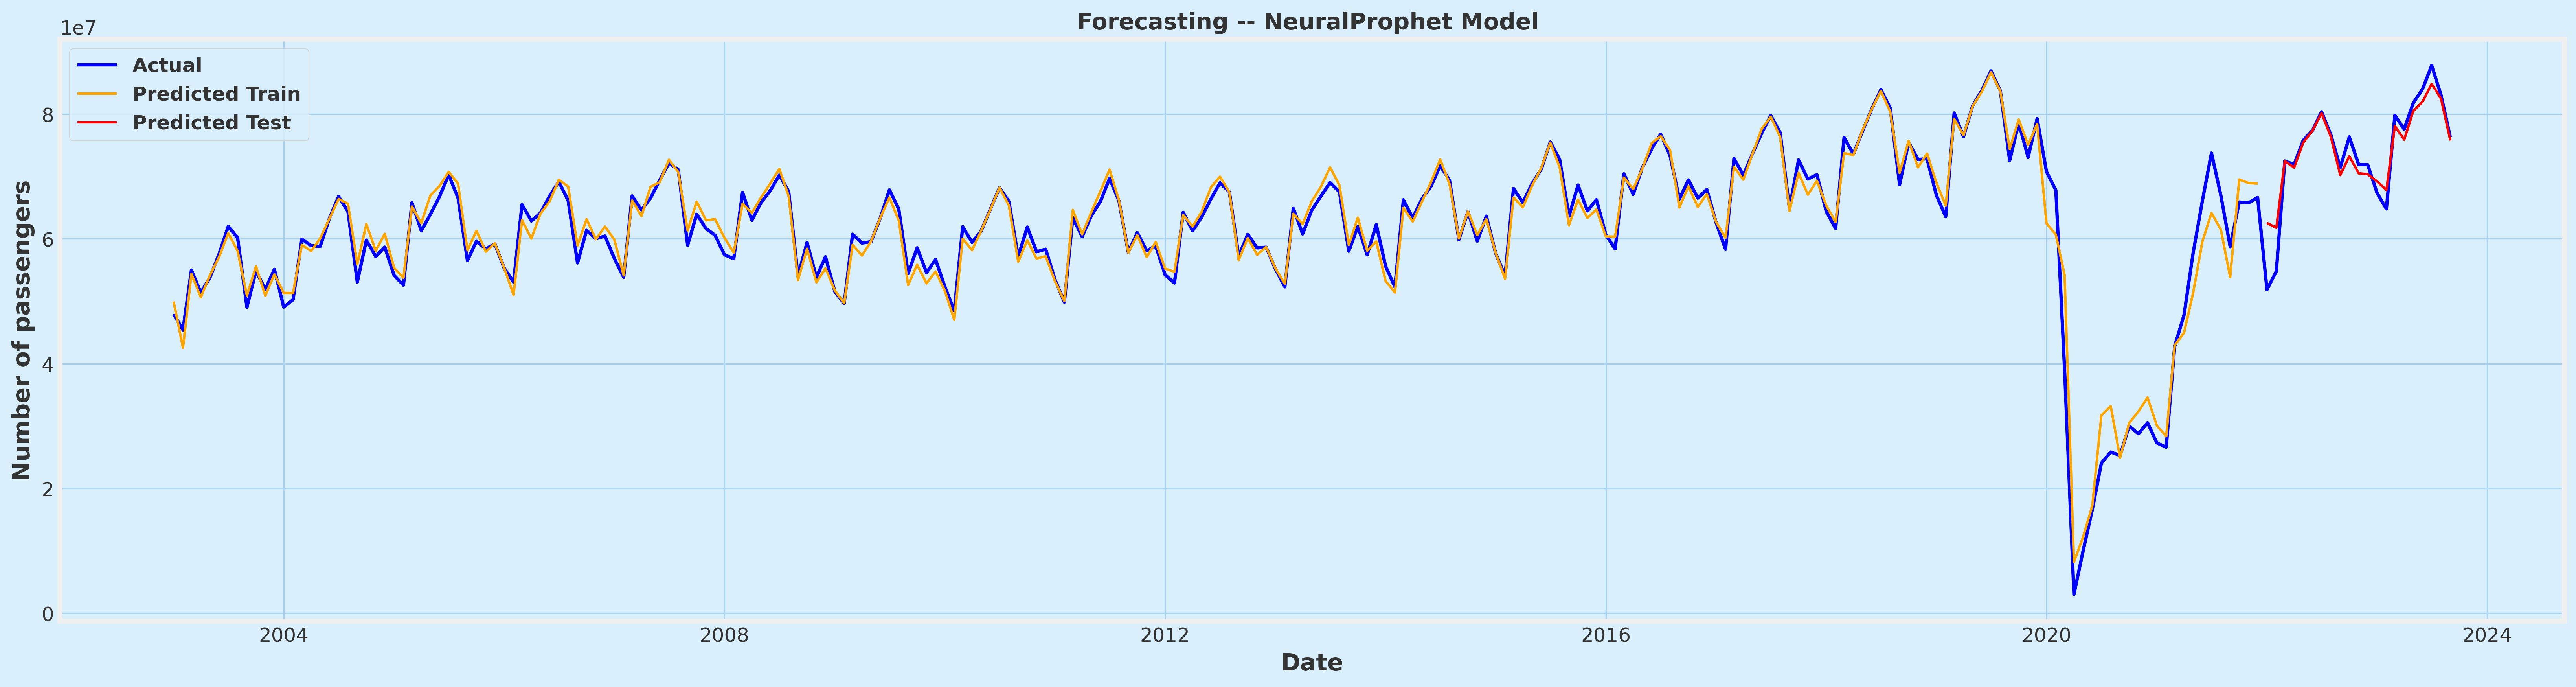
\includegraphics[width=0.8\textwidth]{best_con_covid.png}
    \caption{Predicciones del tercer modelo \textit{NeuralProphet}} 
    \label{fig:fig22}
\end{figure}

Por último, se lanza un modelo siguiendo la estrategia de la sección $~\ref{sec:32}$ al que se le añaden festivos, un regresor futuro (como anteriormente, el número total de vuelos), 200 épocas de entrenamiento y una tasa de aprendizaje de $0,01$. En la Figura $~\ref{fig:fig22}$, se observa que este modelo se ajusta considerablemente mejor a las fluctuaciones y cambios bruscos de los datos, manteniendo la tendencia y estacionalidad anual. Se nota que las predicciones son fieles a la realidad al tener este modelo un error MAPE del $3,12\%$.

\begin{table}[h]
\centering
\begin{tabular}{ccc}
\hline
\textbf{Modelo} & \textbf{MAPE del entrenamiento} & \textbf{MAPE del testeo} \\ \hline
\text{Valores por defecto} & 19,86\% & 35,05\% \\ \hline
\text{Valores por defecto + festivos} & 11,87\% & 15,81\% \\ \hline
\text{Mejores parámetros + festivos} & 3,47\% & 3,12\% \\ \hline
\end{tabular}
\caption{Errores MAPE del modelo NeuralProphet}
\label{tab:error4.2}
\end{table}

Comparando los errores MAPE de los tres modelos (Tabla $~\ref{tab:error4.2}$), se observa \textit{underfitting} y \textit{overfitting} en el primer modelo. El segundo modelo presenta mejoras (aun encontrándose en el límite del \textit{underfitting}), pero se aprecia que los efectos de festivos mejoran el modelo. Se observa que el mejor modelo es el tercero notoriamente, pues presenta unos errores MAPE para el entrenamiento y testeo pequeños. Además, no cae ni en el \textit{overfitting} ni en el \textit{underfitting}, por lo que el tercer modelo es el escogido.



\begin{figure}[h]
    \centering
    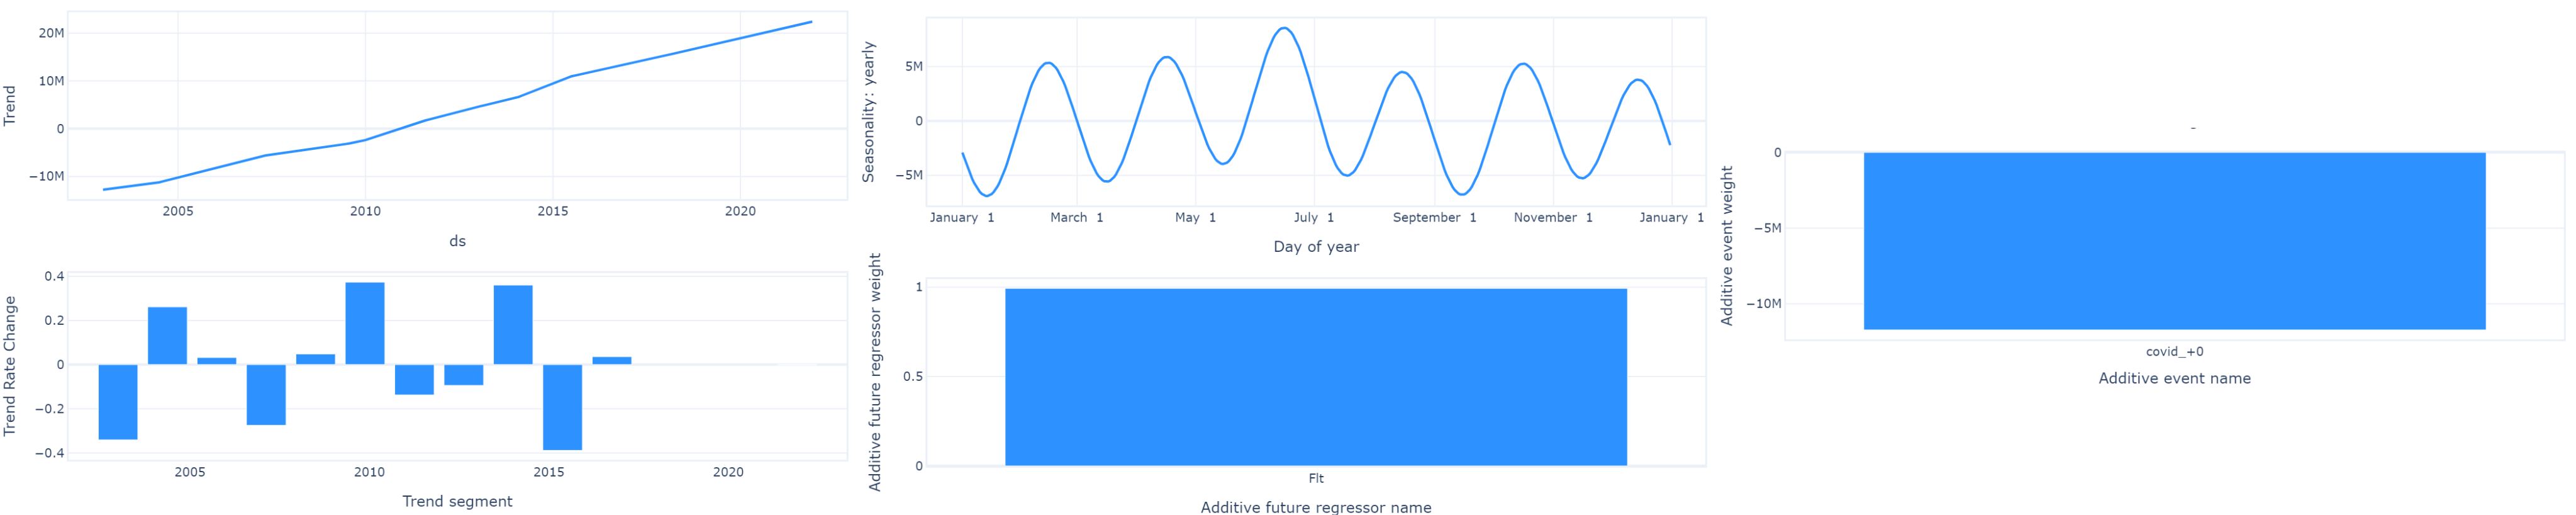
\includegraphics[width=1\textwidth]{best_params_con_covid_dividida1.png}
    \caption{Parámetros del mejor modelo \textit{NeuralProphet}} 
    \label{fig:fig23}
\end{figure}

Finalmente, se puede ver cómo se comportan las componentes del modelo en la Figura $~\ref{fig:fig23}$: se observa una tendencia aproximadamente lineal a lo largo del tiempo. El modelo no refleja la caída durante el COVID, ya que probablemente ha sido capturada por los eventos. Para el cambio de tasa en la tendencia, aunque en general la tendecia se encuentra aumentando, se ven zonas en que crece más y menos lento. Además, para la estacionalidad anual, se aprecian picos en verano y mínimos en enero y septiembre. Para el regresor futuro, se observa un valor muy cercano a 1, lo que indica que el regresor tiene un impacto muy fuerte y directamente proporcional en la predicción. Finalmente, para el evento del COVID, se aprecia un valor aproximado de -10 millones, lo que significa que cada vez que se produce el evento COVID, el modelo resta esta cantidad del valor previsto.




\newpage
\section{Comparación de modelos}\label{sec:38}

A lo largo de este trabajo, se han estudiado fundamentalmente cuatro modelos para la predicción de series temporales.

En cuanto al modelo más tradicional, SARIMA, se basa en procesos lineales previos y necesita transformaciones para hacer la serie estacionaria. Además, una gran cantidad de datos (que no es el caso) requiere un gran tiempo de computación y solo es capaz de modelar un tipo de estacionalidad a la vez.

En lo que respecta a los medelos más actuales, destaca \textit{Prophet} por su fácil interpretabilidad, al poder descomponerse de forma aditiva o multiplicativa, y no necesita que la serie sea estacionaria. Una de sus grandes ventajas frente a otros modelos es la capacidad de añadir festivos, pues permite manejar de forma más efectiva picos o mínimos en los datos. Además, también permite modelar distintos tipos de estacionalidad (anual, semanal, diaria, etc.), aunque en nuestros datos solo aparezca la estacionalidad anual al tener datos mensuales. A pesar de no haber tratado sobre ello en este trabajo, también se les puede añadir variables exógenas.

Por su parte, para el modelo de redes neuronales recurrentes, LSTM, destaca su capacidad para capturar relaciones no lineales y su memoria a largo plazo. Aprende la tendencia y estacionalidad implícitamente de los datos de entrada y también admite variables exógenas. Sin embargo, es un modelo que supone mayor tiempo computacional dado el complicado entrenamiento que requiere y no modela explícitamente la estructura, todo es aprendido. Se suele decir que las redes neuronales son una caja negra dado que no modelan explícitamente las componentes de la serie temporal (tendencia, estacionalidad, etc.). En su lugar, aprenden automáticamente los patrones presentes en los datos ajustando parámetros, sin explicar los factores que contribuyen a la predicción final.

Por último, \textit{NeuralProhet} es el modelo más áctual. Nace como mejora del modelo \textit{Prophet}, para suplir sus limitaciones a la hora de aprender de relaciones no lineales a partir de redes neuronales. Resalta por su capacidad para manejar distintas estacionalidades (incluso las no habituales), por su manejo más flexible de variables exógenas, por su aún facíl uso y por su potencia de modelado. 


\begin{table}[h]
\centering
\begin{tabular}{|c|c|c|c|c|}
\hline
\textbf{Modelo} & \textbf{Tendencia} & \makecell{\textbf{Estacionalidades} \\ \textbf{múltiples}} & \makecell{\textbf{Variables} \\ \textbf{exógenas}} & \textbf{Festivos} \\ \hline
SARIMA & \checkmark\  & \xmark & \xmark\ & \xmark \\ \hline
Prophet & \checkmark\ & \checkmark\ & \checkmark\ & \checkmark \\ \hline
LSTM & \checkmark\ (implícita) & \checkmark\ (implícita) & \checkmark\ & \xmark \\ \hline
NeuralProphet & \checkmark\ & \checkmark\ & \checkmark\ & \checkmark \\ \hline
\end{tabular}
\caption{Comparación de componentes}
\label{tab:componentes}
\end{table}


Por consiguiente, a forma de resumen, en la Tabla $~\ref{tab:componentes}$ se encuentran las componentes de las que dispone cada modelo. Cabe destacar que no se pretende decir que el modelo LSTM las tenga, sino que las aprende de los datos si existen, de manera automática. Además, los modelos que siguen métodos autorregresivos no se descomponen como series temporales, sino que su ajuste depende de los parámetros propios de cada uno de ellos y de los rezagos que usan para inicializarse.

Además, aunque no se ha tratado durante esto a lo largo del trabajo, también es un punto a tener en cuenta el coste computacional que conllevaba la implementación de cada modelo. El modelo SARIMA es sencillo de implementar y no tiene gran coste computacional para una cantidad media/baja de datos. Para el modelo \textit{Prophet}, al no tener demasiados parámetros a ajustar, tiene un coste computacional aceptable para trabajar. Sin embargo, para las redes neuronales, el coste computacional es notablemente alto por la forma en que se entrenan y todos los parámetros que se deben ajustar en cada época de entrenamiento. A la par de ellas, el modelo \textit{NeuralProphet} también tiene un elevado coste computacional al basarse en redes neuronales y tener una alta cantidad de hiperparámetros a ajustar.

Durante el trabajo, se han puesto en práctica cada uno de los modelos con dos \textit{data sets} diferentes, uno con ruido y otro sin ruido (con o sin COVID, respectivamente). Así las cosas, se van a comparar los errores MAPE de cada modelo para los dos conjuntos de datos, con el objetivo de poner de relieve sus puntos fuertes y débiles.

\begin{table}[h]
\centering
\begin{tabular}{|c|c|c|}
\hline
\textbf{Modelo} & \makecell{\textbf{Conjunto de} \\ \textbf{entrenamiento}} & \makecell{\textbf{Conjunto de} \\ \textbf{testeo}} \\ \hline
SARIMA & $4,59\%$ & $1,58\%$  \\ \hline
Prophet & $7,37\%$ & $0,99\%$ \\ \hline
LSTM & $2,72\%$ & $3,34\%$ \\ \hline
NeuralProphet & $1,11\%$ & $1,44\%$ \\ \hline
\end{tabular}
\caption{Comparación de los errores MAPE para el primer \textit{data set} (sin COVID)}
\label{tab:comparacion1}
\end{table}

Como se puede apreciar en los errores MAPE del conjunto de testeo de la Tabla $~\ref{tab:comparacion1}$, para datos sin ruido, cualquiera de los cuatro modelos es apto para usarse. No obstante, el mejor es el modelo \textit{Prophet} por tener el menor error MAPE. Esto pone de manifiesto que dicho modelo sea uno de los primeros a tener en cuenta a la hora de predecir series temporales.

Además, se observa que los errores del conjunto de entrenamiento para los modelos SARIMA y \textit{Prophet} son mayores a los errores del conjunto de testeo. Esto se puede deber a la estabilidad de los datos durante el periodo de testeo, o a que el conjunto de entrenamiento esté sesgado por la volatilidad de los años de entrenamiento, puesto que una mayor volatilidad en el conjunto de entrenamiento puede aumentar el error MAPE. Ocurre lo contrario para los modelos LSTM y \textit{NeuralProphet}, que se puede dar gracias a la redes neuronales, que capturan relaciones no lineales a partir de los datos.

\begin{table}[h]
\centering
\begin{tabular}{|c|c|c|}
\hline
\textbf{Modelo} & \makecell{\textbf{Conjunto de} \\ \textbf{entrenamiento}} & \makecell{\textbf{Conjunto de} \\ \textbf{testeo}} \\ \hline
SARIMA & $8,65\%$ & $12,94\%$  \\ \hline
Prophet & $9,83\%$ & $5,47\%$ \\ \hline
LSTM & $12,02\%$ & $6,44\%$ \\ \hline
NeuralProphet & $3,47\%$ & $3,12\%$ \\ \hline
\end{tabular}
\caption{Comparación de los errores MAPE para el segundo \textit{data set} (sin COVID)}
\label{tab:comparacion2}
\end{table}

Por su parte, para el segundo \textit{data set}, en los errores MAPE del conjunto de testeo de la Tabla $~\ref{tab:comparacion2}$ se notan las limitaciones de los modelos tradicionales, pues el modelo SARIMA tiene un error considerablemente mayor al resto debido a que el COVID sigue siendo complicado de predecir usando los patrones anuales habituales. Para esto datos, el modelo que mejor se adapta a estos repentinos cambios es el modelo \textit{NeuralProphet}, demostrando su flexibilidad a la hora de capturar relaciones no lineales y su capacidad para dar distintas importancias a diferentes momentos en los datos.

Ahora, se aprecia cómo los modelos complejos tienen errores en el entrenamiento mayores que en el testeo, probablemente causado por la volatilidad de los datos para el entrenamiento y la presencia de valores bajos, lo que tiende a incrementar el error relativo. Para intentar mejorar estas condiciones, se podrían comparar los modelos con otras métricas como MSE para evaluar el rendimiento del modelo con mayor fiabilidad. También se podrían llevar a cabo transformaciones logarítmicas para reducir la variabilidad de la serie (para el modelo SARIMA se realizan transformaciones logarítmicas, lo que puede explicar que este modelo siga la normalidad) o incluso cambiar el periodo de entrenamiento. Finalmente, se puede observar que los mejores modelos son aquellos que llevan la componente festivos, y los mejores modelos para ambos datos son \textit{Prophet} y \textit{NeuralProphet}.

\newpage

\section{Conclusiones}\label{sec:39}

Durante el desarrollo de este trabajo, se han estudiado diferentes clases de modelos: desde los procesos más clásicos de series temporales, hasta los más recientes pasando por modelos totalmente diferentes en cuanto a estructura. Se ha desarrollado una ardua labor de investigación de la teoría que hay detrás de cada modelo, a la par de su implementación en \textit{Python} a partir de dos conjuntos de datos relativos al tráfico aéreo mensual de EE.UU. El primer \textit{data set} abarca desde 2003 hasta 2019, y el segundo hasta 2023. Este último contiene los problemáticos años del COVID, por lo que se trata como datos complicados.

En primera lugar, se ha desarrollado el modelo clásico SARIMA y se ha comprobado que, para conjuntos de datos complicados, presentan diversas limitaciones, pues relacionan las observaciones y sus retardos de forma lineal y solo son capaces de modelar una estacionalidad a la vez. A continuación, se sigue la mejora en cuanto a rendimiento e interpretabilidad que supone el modelo \textit{Prophet} en comparación al SARIMA, ya que tiene una descomposición aditiva o multiplicativa, permite añadir al modelo los efectos festivos futuros a tener en cuenta  y es capaz de modelar diferentes estacionalidades en un mismo tiempo. Posteriormente, se han introducido la teoría general de las redes neuronales, centrándose en las redes neuronales recurrentes hasta llegar al modelo LSTM, que se caracteriza en este trabajo por su distintiva forma de entrenar y predecir. Destaca su capacidad para analizar relaciones no lineales y su forma de construir el modelo, siempre a partir de los datos, a la par de su enorme costo computacional. Por último, se culmina el estudio de modelos  con el que es el objeto de estudio de este trabajo, el modelo \textit{NeuralProphet}, que se puede definir \textit{grosso modo} como la unión del modelo Prophet y las redes neuronales. Este modelo tiene lo mejor de ambos: puede capturar distintos tipos de tendencias, puede captar diferentes patrones estacionales y trabajar con ellos simultáneamente y sigue teniendo facilidad de interpretación y uso.

Gracias a la implementación practica en \textit{Python} de los algoritmos desarrollados, se ha llegado a la conclusión de que el modelo \textit{Prophet} es una de las mejores opciones para empezar a estudiar una serie temporal, y si los datos son complicados, una aún mejor opción es el modelo \textit{NeuralProphet}. 


\begin{figure}[h]
    \centering
    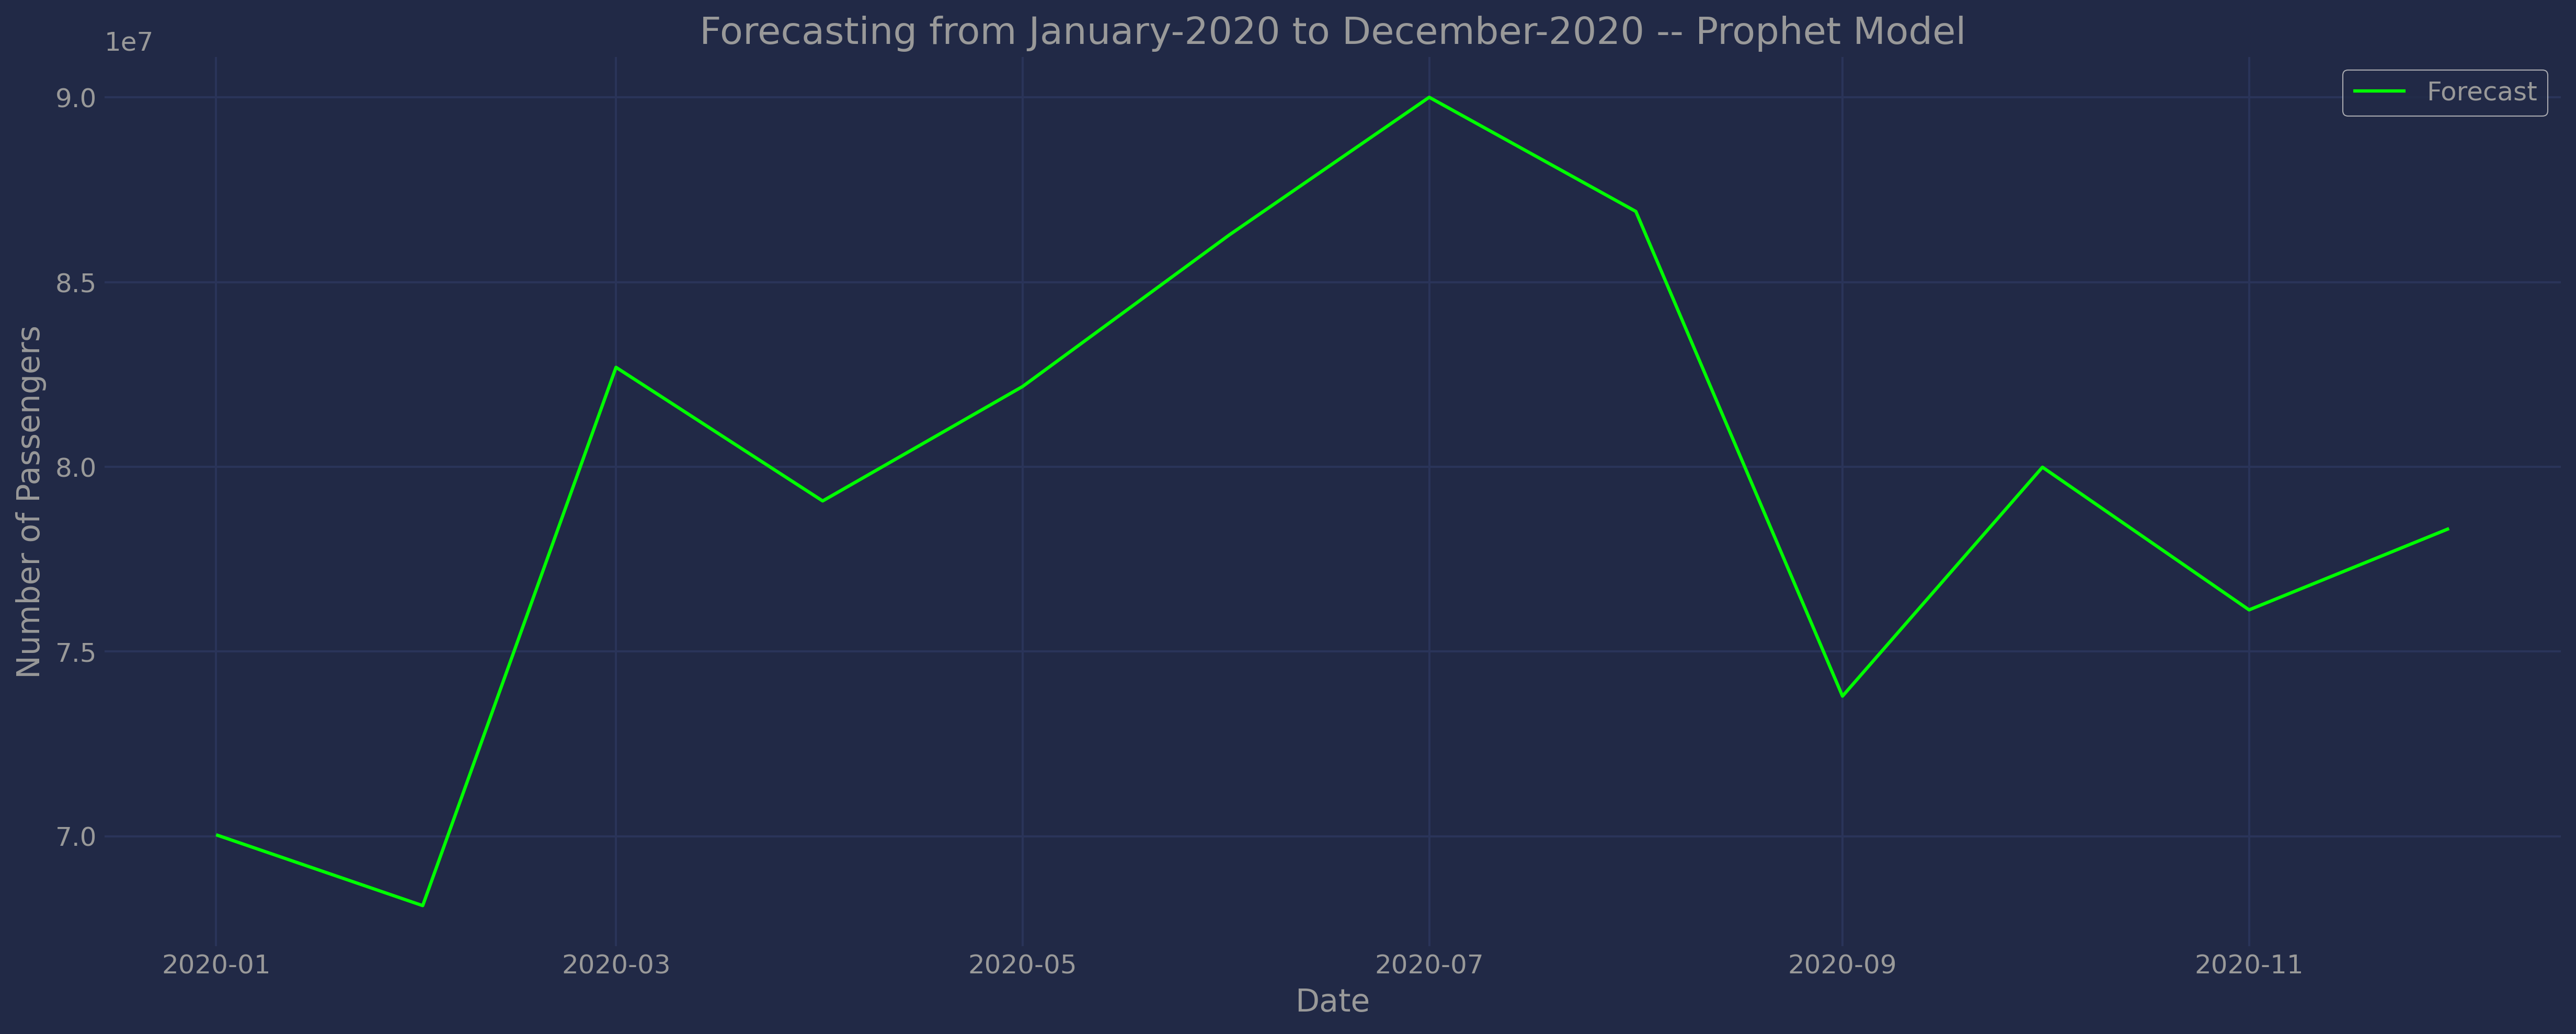
\includegraphics[width=0.8 \textwidth]{final_pred_prophet.png}
    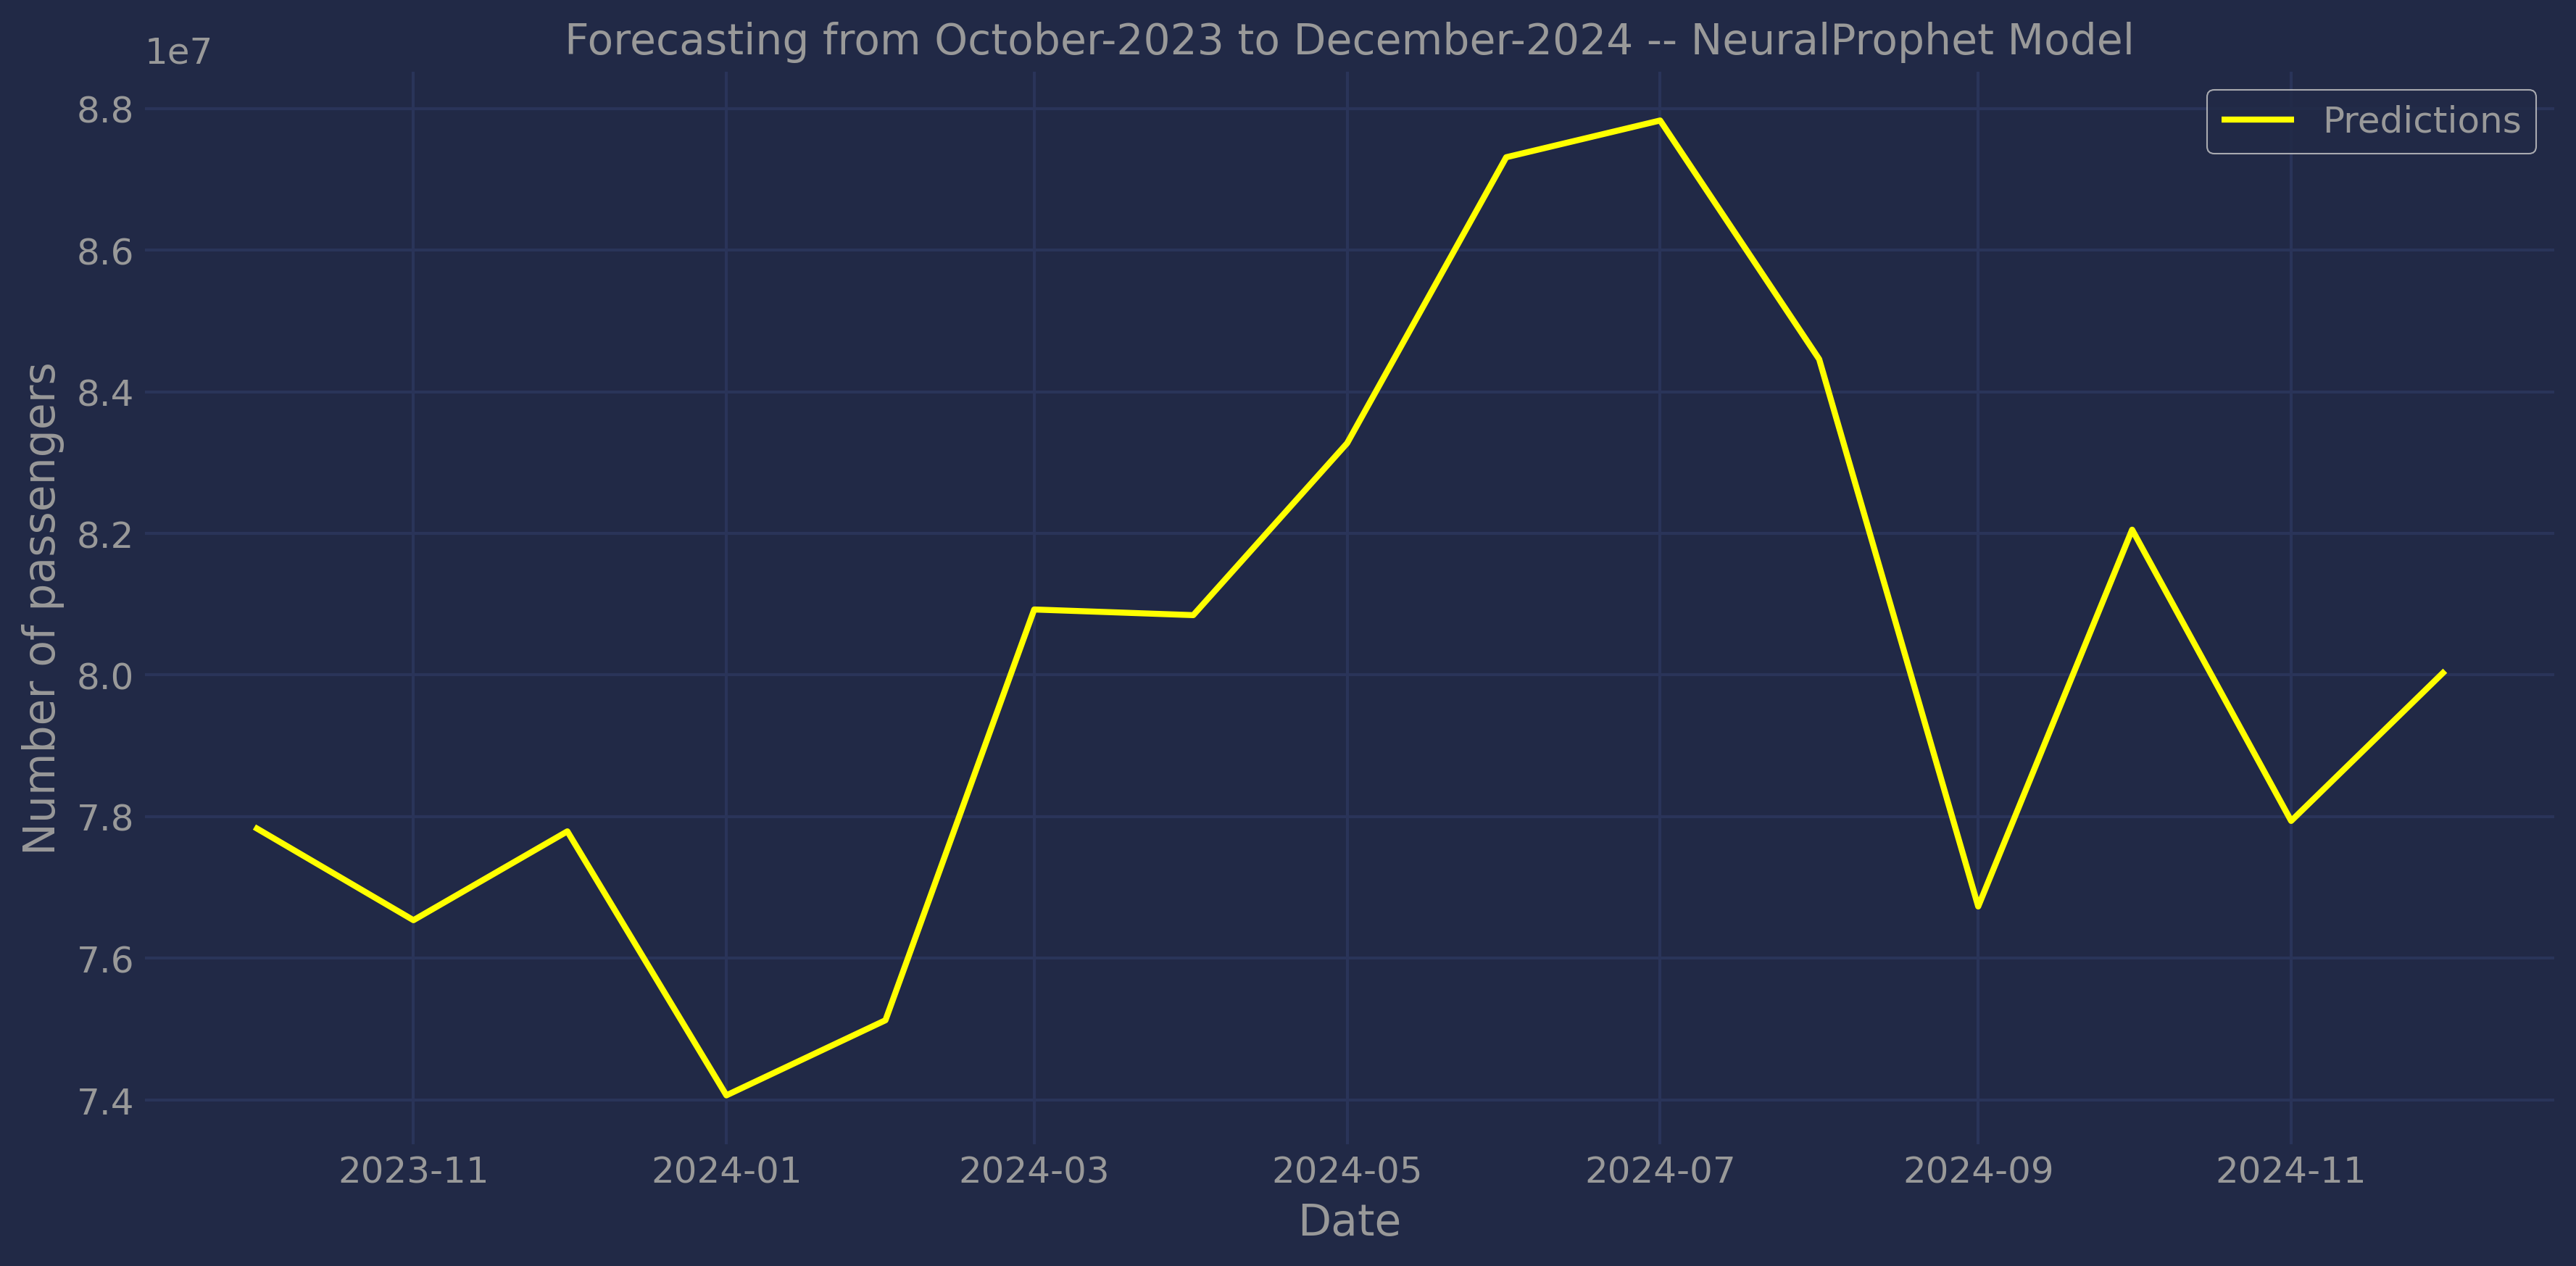
\includegraphics[width=0.8 \textwidth]{final_pred_neuralprophet.png}
    \caption{Predicciones con los mejores modelos} 
    \label{fig:fig30}
\end{figure}

Para el primer conjunto de datos, se puede en la primera imagen de la Figura $~\ref{fig:fig30}$ la predicción para el año 2022 con el modelo \textit{Prophet}. Se observa cómo se esperaba que el número de pasajeros por mes para ese año estuviera entre $65-90$ millones, algo más que en años anteriores. Por otro lado, para el segundo conjunto de datos, se puede apreciar en la segunda imagen de la Figura $~\ref{fig:fig30}$ la predicción para los tres últimos meses de 2023 y todo 2024, con el modelo \textit{NeuralProphet}. Se ve que el número esperado de pasajeros por mes para ese periodo de tiempo se sitúa entre $74-88$ millones, algo ligeramente superior a años anteriores.

Se puede observar cómo la estimación del número de pasajeros para 2024 casi se asimila a la de 2022, lo que nos lleva a pensar en el gran efecto del COVID en este sector, que en 2024 todavía no estaría del todo recuperado.

Para concluir todo el trabajo, todo lo aquí realizado se podría extender a diferentes modelos de negocio. En este caso, solo se tenía un producto, que es el número de pasajeros para las aerolíneas estadounidenses. Sin embargo, para otros modelos de negocios, como el de una empresa que tenga tiendas en diferentes lugares, se podrían automatizar estos modelos para cada producto de las tiendas de forma no supervisada.

En particular, en empresas que disponen de variedad de productos y tiendas distribuidas en diversas zonas, resultaría interesante automatizar el proceso de generación de modelos predictivos para cada combinación de producto y localización. Esto permitiría realizar predicciones específicas y personalizadas de forma no supervisada, sin apenas intervención manual y aumentando significativamente la eficiencia y precisión de la planificación empresarial. De la misma forma, la automatización de esto podría facilitar la detección de irregularidades, la optimización del inventario y del espacio de almacenamiento y la mejora de las estrategias comerciales basadas en análisis predictivos a gran escala. También, podría resultar interesentante escoger varios modelos por apartado y no centrarse en uno solo, como se ha hecho a lo largo de este trabajo.

\newpage


\addcontentsline{toc}{section}{Referencias}
\begin{thebibliography}{100}


\bibitem{rnn1}
Amat Rodrigo, J. and Carazo, F., Deep Learning para la predicción de series temporales: Redes Neuronales Recurrentes (RNN) y Long Short-Term Memory (LSTM). \url{https://cienciadedatos.net/documentos/py54-forecasting-con-deep-learning} (Consultado el 3 de mayo de 2025).

\bibitem{redes5}
Ali, M., Introducción a las funciones de activación en las redes neuronales. \url{https://www.datacamp.com/es/tutorial/introduction-to-activation-functions-in-neural-networks} (Consultado el 3 de mayo de 2025).

\bibitem{sarima1}
Brockwell, P.J. and Davis, R.A. (1987) \textit{Time Series: Theory and Methods}. Springer.

\bibitem{prophet2}
Castellon, N. (2024) Time Series Forecasting Prophet, in \url{https://www.youtube.com/@narencastellon}. (Consultado el 3 de mayo de 2025 en \url{https://www.youtube.com/watch?v=UB9S3JPdNXU}).

\bibitem{rnn4}
Codificando Bits (2024) Forecasting con Redes LSTM (parte 4): modelo univariado + multistep, in \url{https://www.youtube.com/@CodificandoBits}. (Consultado el 3 de mayo de 2025 en \url{https://www.youtube.com/watch?v=TEzTfl_E-3o}).

\bibitem{redes2}
DalpMaths (2020) Backpropagation: (parte 1), in \url{https://www.youtube.com/@DalpMaths}. (Consultado el 3 de mayo de 2025 en \url{https://www.youtube.com/watch?v=wWV2qroGUMo&list=PLxJ9ooR1g5bhmhequ3e7LttlKmrnLYQGl&index=6}).

\bibitem{redes3}
DalpMaths (2020) Backpropagation: (parte final), in \url{https://www.youtube.com/@DalpMaths}. (Consultado el 3 de mayo de 2025 en \url{https://www.youtube.com/watch?v=LBGFjOgea1M&list=PLxJ9ooR1g5bhmhequ3e7LttlKmrnLYQGl&index=17}).

\bibitem{rnn3}
Ghojogh, B. (2024) Deep Learning, F23(7): Backpropagation Through Time, RNN, LSTM, GRU, Bidirectional LSTM, ELMo, in \url{https://www.youtube.com/@benyaminghojogh}. (Consultado el 3 de mayo de 2025 en \url{https://www.youtube.com/watch?v=o2W3zc730CE}).

\bibitem{redes4}
Goodfellow, I., Deep Feedforward Networks in \textit{Deep Learning}, Goodfellow, I., Bengio, Y. and Courville, A. (2016) \textit{pp.164-223}.

\bibitem{rnn2}
Goodfellow, I., Sequence Modeling: Recurrent and Recursive Nets in \textit{Deep Learning}, Goodfellow, I., Bengio, Y. and Courville, A. (2016) \textit{pp.367-415}.

\bibitem{redes1}
IBM, What is a neural network? \url{https://www.ibm.com/think/topics/neural-networks} (Consultado el 3 de mayo de 2025).

\bibitem{prophet1}
Taylor, S.J. and Letham, B. (2018) Forecasting at Scale, in \url{https://www.researchgate.net/}. (Consultado el 3 de mayo de 2025 en \url{https://www.researchgate.net/publication/344989540_Forecasting_at_scale}).

\bibitem{np1}
Triebe, O., Hewamalage, H., Pilyugina, P., Laptev, N., Bergmeir, C. and Rajagopal, R. (2021) NeuralProphet: Explainable Forecasting at Scale, in \url{https://arxiv.org/}. (Consultado el 3 de mayo de 2025 en \url{https://arxiv.org/abs/2111.15397}).

\bibitem{np2}
Triebe, O., Selecting the Hyperparameters. \url{https://neuralprophet.com/how-to-guides/feature-guides/hyperparameter-selection.html} (Consultado el 3 de mayo de 2025).

\end{thebibliography}

\newpage
\appendix

\section{Detalles del desarrollo del trabajo}
Todo el códido desarrollado durante el trabajo para llevar a cabo los diferentes modelos, obtener resultados y dibujar gráficas se puede encontrar fácilmente en la carpeta de \textit{GitHub} (\url{https://github.com/juanfran12345/TFG}). Además, el código se encuentra dividio en diferentes \textit{notebooks}, organizados según las secciones del proyecto y el conjunto de datos. En total, ocho \textit{notebooks}.

Los datos usados han sido proporcionados por \textit{Kaggle} y se encuentras en el siguiente enlace: \href{https://www.kaggle.com/datasets/yyxian/u-s-airline-traffic-data}{https://www.kaggle.com/datasets/yyxian/u-s-airline-traffic-data}.

\begin{table}[ht] 
\centering
\begin{tabular}{lc} 
  \hline
 Tarea & Tiempo (horas) \\ 
  \hline
Recopilación de materiales &   20 \\ 
Estudio de bibliografía &   30 \\ 
Elaboración de código y gráficos &  40 \\ 
Redacción de la memoria &  60 \\
 \hline
Total & 150\\
\hline
\end{tabular}
\caption{Tiempo aproximado de dedicación al trabajo} \label{tab{02}}
\end{table}

\begin{table}[ht] 
\centering
\begin{tabular}{llll} 
  \hline
 Asignatura & Páginas & Descripción  \\ 
  \hline
Series Temporales   & 9-12 & Definición de series temporales y procesos estacionarios. \\
& & Procesos ARIMA y SARIMA. \\
& & Metodología de Box-Jenkins.  \\
Optimización II  & 25-36 & Funcionamiento de algoritmos de optimización. \\
Análsis de datos I  & General & Relación general de los aspectos discutidos. \\ 
Análsis de datos II & General & Interpretación y discusión de los modelos. \\ 
\hline
\end{tabular}
\caption{Asignaturas relacionadas con el trabajo} \label{tab{03}}
\end{table}

\newpage

\section{Terminología}

Para un correcto entendimiento del trabajo, se considera oportuno definir los siguientes términos en ciencia de datos que se mencionan a lo largo del mismo:

\begin{definition}\label{def:overfitting}
Se dice que un modelo cae en \textit{overfitting} (sobreajuste) cuando un modelo aprende con demasiada precisión los datos de entrenamiento, lo que impide generalizar correctamente nuevos datos. Se suele notar cuando el error para el conjunto de entramiento es considerablemente menor al del conjunto de prueba.
\end{definition}

\begin{definition}\label{def:underfitting}
Se dice que un modelo cae en \textit{underfitting} (subeajuste) cuando un modelo no logra capturar las relaciones fundamentales en los datos de entrenamiento, lo que resulta en un rendimiento deficiente tanto en los datos de entrenamiento como en los nuevos. Se suele notar cuando los errores para el conjunto de entramiento y el conjunto de prueba son notablemente altos.
\end{definition}

\begin{definition} \label{def:criterios}
Para seleccionar el modelo SARIMA que mejor se ajuste a los datos, se usan los criterios AIC, AICc y BIC.

\begin{enumerate} 
    \item Criterio AIC (Criterio de Información de Akaike):es una medida de la calidad relativa de un modelo que combina la bondad del ajuste y la complejidad del modelo. Se utiliza para seleccionar el modelo que mejor se ajusta a los datos con el menor número de parámetro.
    \item Criterio AICc: es la versión corregida del AIC que tiene en cuenta el tamaño de la muestra.
    \item Criterio BIC (Criterio de Información Bayesiano): es una medida de la calidad relativa de un modelo que combina la bondad del ajuste y la complejidad del modelo utilizando un enfoque bayesiano. Se utiliza para seleccionar el modelo que mejor se ajusta a los datos con una penalización adicional por complejidad, favoreciendo modelos más simples en comparación con el AIC.
\end{enumerate}
\end{definition}

\begin{definition} \label{def:dickey}
La prueba de Dickey-Fuller Aumentado es un test estadístico que determina si una serie temporal es estacionaria.
\end{definition}

\begin{definition} \label{def:val}
La validación cruzada temporal es una técnica de evaluación de modelos de aprendizaje automático, especialmente utilizada en series temporales, que respeta orden cronológico de los datos. En lugar de dividir aleatoriamente los datos como en la validación cruzada tradicional, se utiliza una ventana deslizante a través de las observaciones pasadas para entrenar y probar el modelo, respetando la dependencia temporal de los datos. 
\end{definition}

\begin{definition} \label{def:regularizacion}
Una función de regularización es un término adicional que se añade a la función de pérdida durante el entrenamiento de un modelo de aprendizaje automático o red neuronal, principalmente para evitar el sobreajuste.
\end{definition}



\end{document}